%% This is the ctufit-thesis example file. It is used to produce theses
%% for submission to Czech Technical University, Faculty of Information Technology.
%%
%% Get the newest version from
%% https://gitlab.fit.cvut.cz/theses-templates/FITthesis-LaTeX
%%
%%
%% Copyright 2021, Eliska Sestakova and Ondrej Guth
%%
%% This work may be distributed and/or modified under the
%% conditions of the LaTeX Project Public Licenese, either version 1.3
%% of this license or (at your option) any later version.
%% The latest version of this license is in
%%  https://www.latex-project.org/lppl.txt
%% and version 1.3 or later is part of all distributions of LaTeX
%% version 2005/12/01 or later.
%%
%% This work has the LPPL maintenance status `maintained'.
%%
%% The current maintainer of this work is Ondrej Guth.
%% Contact ondrej.guth@fit.cvut.cz for bug reports.
%% Alternatively, submit bug reports into the tracker at
%% https://gitlab.fit.cvut.cz/theses-templates/FITthesis-LaTeX/issues
%%
%%

% arara: pdflatex
% arara: biber
% arara: pdflatex
% arara: pdflatex

%%%%%%%%%%%%%%%%%%%%%%%%%%%%%%%%%%%%%%%%%
% CLASS OPTIONS
% language: czech/english/slovak
% thesis type: bachelor/master/dissertation
% colour: bw for black&white OR no option for default colour scheme
% electronic or printed: oneside/twoside (default)
%%%%%%%%%%%%%%%%%%%%%%%%%%%%%%%%%%%%%%%%%
\documentclass[slovak,master,unicode,oneside,bw]{ctufit-thesis}

%%%%%%%%%%%%%%%%%%%%%%%%%%%%%%%%%%
% FILL IN THIS INFORMATION
%%%%%%%%%%%%%%%%%%%%%%%%%%%%%%%%%%
\ctufittitle{Automatická detekcia pohybových artefaktov v EKG signáli z~nositeľného snímača pomocou metód umelej inteligencie} % replace with the title of your thesis
\ctufitauthorfull{Bc. Veronika Kalousková} % replace with your full name (first name(s) and then family name(s) / surname(s)) including academic degrees
\ctufitauthorsurnames{Kalousková} % replace with your surname(s) / family name(s)
\ctufitauthorgivennames{Veronika} % replace with your first name(s) / given name(s)
\ctufitsupervisor{doc.\,Ing.\,Pavel Smrčka,\,Ph.D.} % replace with name of your supervisor/advisor (include academic degrees)
\ctufitdepartment{Katedra aplikovanej matematiky} % replace with the department of your defence
\ctufityear{2024} % replace with the year of your defence
\ctufitdeclarationplace{Prahe} % replace with the place where you sign the declaration
\ctufitdeclarationdate{\today} % replace with the date of signature of the declaration
\ctufitabstractCZE{Práca sa zaoberá automatickou detekciou pohybových artefaktov z elektrokardiogramu. V rámci riadeného experimentu bola vytvorená anotovaná dátová sada obsahujúca 4602 segmentov EKG signálu dlhých dve sekundy. Záznamy boli vyhotovené počas fyzickej aktivity rôznych intenzít, segmenty sú klasifikované podľa štyroch rôznych stupňov rušenia. Na meranie bol použitý nositeľný snímač a tri rôzne druhy elektród - Ag/AgCl, chróm-niklové a textilné elektródy - pričom posledné vykazujú najväčšiu odolnosť voči pohybovým artefaktom. Navrhnuté boli dva hlboké konvolučné modely, jeden na klasifikáciu fyzických aktivít, druhý na klasifikáciu pohybových artefaktov. Presnosť klasifikácie pohybových aktivít dosahuje 85,67 \%, presnosť klasifikácie pohybových artefaktov 87,62 \%. Výsledný model dokáže odlíšiť segmenty s čitateľným a nečitateľným srdečným rytmom s presnosťou 98,70 \%.}
\ctufitabstractENG{The thesis addresses the topic of automatic artefact detection in electrocardiograms. A controlled experiment was conducted, resulting in a labeled dataset comprising 4602 two seconds long ECG segments. The recordings were acquired during physical activities of varying degrees, and~individual segments were categorized into four distinct classes based on the extent of the artefacts present. A wearable sensor with three different types of electrodes was used - Ag/AgCl, chrome-nickel, and textile - the latter of which revealed superior performance in mitigating motion artefacts. Two deep convolutional models were proposed: one for classifying physical activities and another for motion artefact classification. Results demonstrate an accuracy of 85.67~\% for~physical activity classification and 87.62 \% for motion artefact classification. Furthermore, the model exhibits an accuracy of 98.70 \% in correctly identifying segments with detectable and~non-detectable heart rates.}
\ctufitkeywordsCZE{pohybový artefakt, elektrokardiografia, klasifikácia EKG, automatická detekcia artefaktov v EKG, spracovanie biosignálov, konvolučná neurónová sieť, hlboké učenie}
\ctufitkeywordsENG{motion artefact, electrocardiography, ECG classification, biosignal processing, automatic artefact detection in ECG,  convolutional neural network, deep learning}
%%%%%%%%%%%%%%%%%%%%%%%%%%%%%%%%%%
% END FILL IN
%%%%%%%%%%%%%%%%%%%%%%%%%%%%%%%%%%

%%%%%%%%%%%%%%%%%%%%%%%%%%%%%%%%%%
% CUSTOMIZATION of this template
% Skip this part or alter it if you know what you are doing.
%%%%%%%%%%%%%%%%%%%%%%%%%%%%%%%%%%

\RequirePackage{iftex}[2020/03/06]
\iftutex % XeLaTeX and LuaLaTeX
    \RequirePackage{ellipsis}[2020/05/22] %ellipsis workaround for XeLaTeX
\else
    \RequirePackage[utf8]{inputenc}[2018/08/11] %this file encoding
    \RequirePackage{lmodern}[2009/10/30] % vector flavor of Computer Modern font
\fi

% hyperlinks
\RequirePackage[pdfpagelayout=TwoPageRight,colorlinks=false,allcolors=decoration,pdfborder={0 0 0.1}]{hyperref}[2020-05-15]

% uncomment the following to hide all hyperlinks
% \RequirePackage[pdfpagelayout=TwoPageRight,hidelinks]{hyperref}[2020-05-15]

\RequirePackage{pdfpages}[2020/01/28]

\setcounter{secnumdepth}{4} % numbering sections; 4: subsubsection



%%%%%%%%%%%%%%%%%%%%%%%%%%%%%%%%%%
% CUSTOMIZATION of this template END
%%%%%%%%%%%%%%%%%%%%%%%%%%%%%%%%%%


%%%%%%%%%%%%%%%%%%%%%%
% DEMO CONTENTS SETTINGS
% You may choose to modify this part.
%%%%%%%%%%%%%%%%%%%%%%
\usepackage{dirtree}
\usepackage{lipsum,tikz}
\usepackage{csquotes}
\usepackage[style=iso-numeric]{biblatex}
\addbibresource{text/bib-database.bib}
\usepackage{listings} % typesetting of sources
\usepackage[skip=8pt, indent=40pt]{parskip}
\usepackage{array}

\newcolumntype{L}[1]{>{\raggedright\arraybackslash}m{#1}}
\newcolumntype{C}[1]{>{\centering\arraybackslash}m{#1}}
\newcolumntype{R}[1]{>{\raggedleft\arraybackslash}m{#1}}

%\usepackage[newfloat]{minted}\captionsetup[listing]{position=top} % typesetting of sources

% Force figure positions
\usepackage{float}

% Force footnote positions - not matter the length do not split into multiple pages
\interfootnotelinepenalty=10000
\usepackage[bottom]{footmisc}

%theorems, definitions, etc.
\theoremstyle{plain}
\newtheorem{theorem}{Veta}
\newtheorem{lemma}[theorem]{Tvrdenie}
\newtheorem{corollary}[theorem]{Dôsledok}
\newtheorem{proposition}[theorem]{Návrh}
\newtheorem{definition}[theorem]{Definícia}
\theoremstyle{definition}
\newtheorem{example}[theorem]{Príklad}
\theoremstyle{remark}
\newtheorem{note}[theorem]{Poznámka}
\newtheorem*{note*}{Poznámka}
\newtheorem{remark}[theorem]{Pozorovanie}
\newtheorem*{remark*}{Pozorovanie}
\numberwithin{theorem}{chapter}
%theorems, definitions, etc. END
%%%%%%%%%%%%%%%%%%%%%%
% DEMO CONTENTS SETTINGS END
%%%%%%%%%%%%%%%%%%%%%%

\begin{document} 
\frontmatter\frontmatterinit % do not remove these two commands

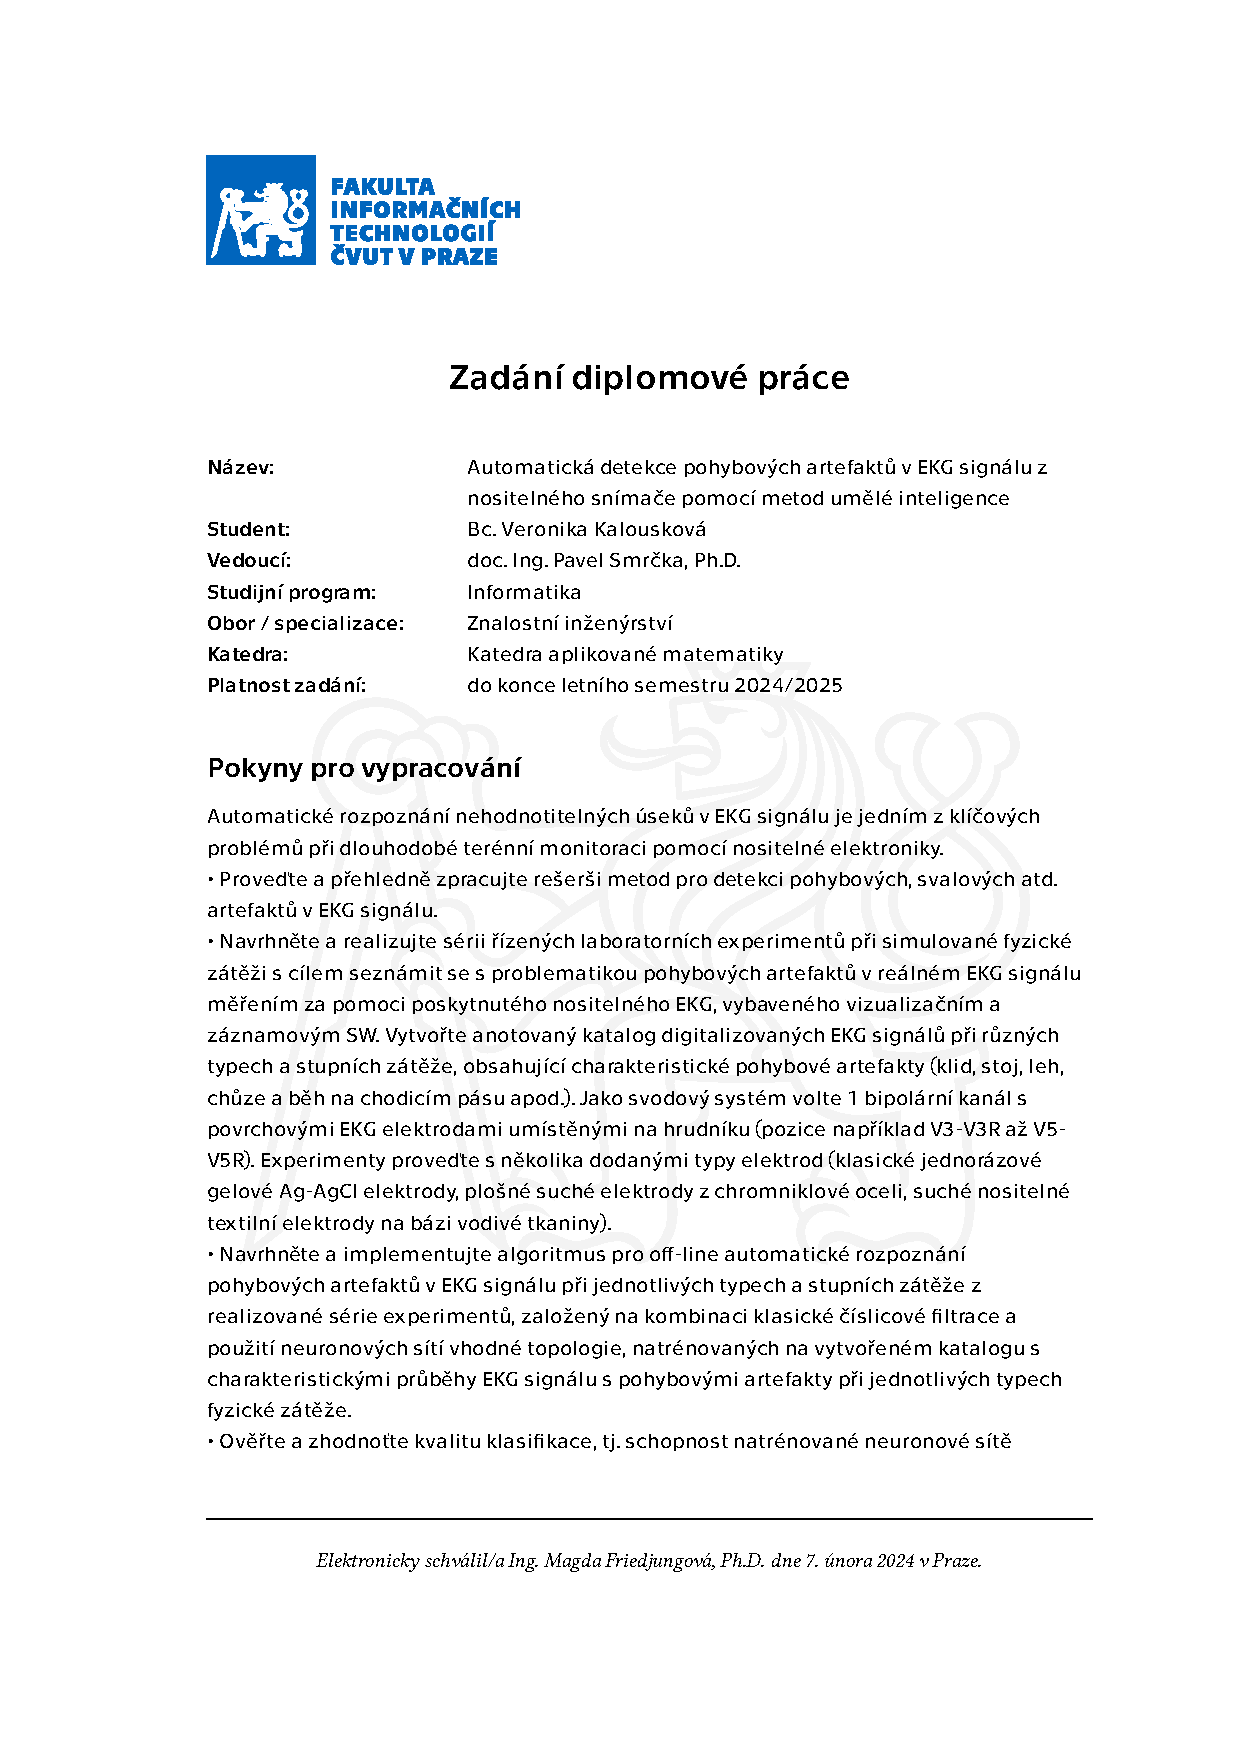
\includepdf[pages={1-}]{kalouver-assignment.pdf} % replace that file with your thesis assignment provided by study office

\thispagestyle{empty}\cleardoublepage\maketitle % do not remove these three commands

\imprintpage % do not remove this command

\tableofcontents % do not remove this command
%%%%%%%%%%%%%%%%%%%%%%
% list of other contents: figures, tables, code listings, algorithms, etc.
% add/remove commands accordingly
%%%%%%%%%%%%%%%%%%%%%%
\listoffigures % list of figures
\begingroup
\let\clearpage\relax
\listoftables % list of tables
% \lstlistoflistings % list of source code listings generated by the listings package
% \listoflistings % list of source code listings generated by the minted package
\endgroup
%%%%%%%%%%%%%%%%%%%%%%
% list of other contents END
%%%%%%%%%%%%%%%%%%%%%%

%%%%%%%%%%%%%%%%%%%
% ACKNOWLEDGMENT
% FILL IN / MODIFY
% This is a place to thank people for helping you. It is common to thank your supervisor.
%%%%%%%%%%%%%%%%%%%
\begin{acknowledgmentpage}
	Rada by som poďakovala vedúcemu práce doc. Ing. Pavlovi Smrčkovi, Ph.D. za odborné rady a konzultácie ohľadom tvorby práce a experimentu. Zároveň by som chcela poďakovať Ing. Radimovi Klimentovi, Ph.D. za cenné rady týkajúce sa využitia metód umelej inteligencie v oblasti biologických signálov. Špeciálne poďakovanie patrí aj všetkým účastníkom experimentu, bez ktorých by táto práca nebola možná.
\end{acknowledgmentpage} 
%%%%%%%%%%%%%%%%%%%
% ACKNOWLEDGMENT END
%%%%%%%%%%%%%%%%%%%


%%%%%%%%%%%%%%%%%%%
% DECLARATION
% FILL IN / MODIFY
%%%%%%%%%%%%%%%%%%%
% INSTRUCTIONS
% ENG: choose one of approved texts of the declaration. DO NOT CREATE YOUR OWN. Find the approved texts at https://courses.fit.cvut.cz/SFE/download/index.html#_documents (document Declaration for FT in English)
% CZE/SLO: Vyberte jedno z fakultou schvalenych prohlaseni. NEVKLADEJTE VLASTNI TEXT. Schvalena prohlaseni najdete zde: https://courses.fit.cvut.cz/SZZ/dokumenty/index.html#_dokumenty (prohlášení do ZP)
\begin{declarationpage}

Prehlasujem, že som predloženú prácu vypracovala samostatne a že som uviedla všetky použité informačné zdroje v súlade s Metodickým pokynom o dodržiavaní etických princípov pri príprave vysokoškolských záverečných prác. 

Beriem na vedomie, že sa na moju prácu vzťahujú práva a povinnosti vyplývajúce zo zákona č. 121/2000 Sb., autorského zákona, v znení neskorších predpisov, hlavne skutočnosť, že České vysoké učení technické v Praze má právo na uzavretie licenčnej zmluvy o využití tejto práce ako školského diela podľa § 60 odst. 1 citovaného zákona.

\end{declarationpage}
%%%%%%%%%%%%%%%%%%%
% DECLARATION END
%%%%%%%%%%%%%%%%%%%

\printabstractpage % do not remove this command

%%%%%%%%%%%%%%%%%%%
% SUMMARY
% FILL IN / MODIFY
% OR REMOVE ENTIRELY (upon agreement with your supervisor)
% (appropriate to remove in most theses)
%%%%%%%%%%%%%%%%%%%
% \begin{summarypage}
% \section*{Summary section}
% 
% \lipsum[1][1-8]
% 
% \section*{Summary section}
% 
% \lipsum[2][1-6]
% 
% \section*{Summary section}
% 
% \lipsum[3]
% 
% \section*{Summary section}
% 
% \lipsum[2]
% 
% \section*{Summary section}
% 
% \lipsum[1][1-8] Lorem lorem lorem.
% \end{summarypage}
%%%%%%%%%%%%%%%%%%%
% SUMMARY END
%%%%%%%%%%%%%%%%%%%

%%%%%%%%%%%%%%%%%%%
% ABBREVIATIONS
% FILL IN / MODIFY
% OR REMOVE ENTIRELY
% List the abbreviations in lexicography order.
%%%%%%%%%%%%%%%%%%%
\chapter{Zoznam skratiek}
	
\begin{tabular}{rl}
AD & Analógovo-digitálny\\
Ag & Striebro\\
AgCl & Chlorid strieborný\\
ANN & Umelá neurónová sieť\\
BPTT & Spätné šírenie chyby v čase\\
CMRR & Činiteľ potlačenia súfázového signálu\\
CNN & Konvolučná neurónová sieť\\
EKG & Elektrokardiogram\\
FN & False negative\\
FP & False positive\\
ICA & Analýza nezávislých komponentov\\
IZS & Integrovaný záchranný systém\\
LSTM & Long short-term memory\\
RNN & Rekurentná neurónová sieť\\
SQA & Posudzovanie kvality signálu\\
SVM & Support vector machine\\
TN & True negative\\
TP & True positive\\
\end{tabular}
%%%%%%%%%%%%%%%%%%%
% ABBREVIATIONS END
%%%%%%%%%%%%%%%%%%%

\mainmatter\mainmatterinit % do not remove these two commands

%%%%%%%%%%%%%%%%%%%
% THE THESIS
% MODIFY ANYTHING BELOW THIS LINE
%%%%%%%%%%%%%%%%%%%

% Do not forget to include Introduction
%---------------------------------------------------------------
% \chapter{Introduction}
% uncomment the following line to create an unnumbered chapter
\chapter*{Úvod}\addcontentsline{toc}{chapter}{Úvod}\markboth{Úvod}{Úvod}
%---------------------------------------------------------------
\setcounter{page}{1}

Efektívna filtrácia pohybových a iných artefaktov v elektrokardiografickom zázname pri dlhodobom terénnom monitorovaní športovcov, alebo zásahových zložiek, zostáva nevyriešeným problémom. Keďže sa frekvenčné spektrum pohybových artefaktov do veľkej miery prekrýva s~frekvenčným spektrom EKG signálu, filtrácia bez straty veľkého množstva klinicky významnej informácie nie je možná. Pri dlhodobom terénnom monitorovaní vitálnych funkcií pomocou nositeľnej elektroniky, kedy nie je nutne potrebné analyzovať celý zaznamenaný signál, je žiadúce úseky signálu, ktoré sú príliš znečistené pohybovým artefaktom, odstrániť, a sústrediť sa analýzu zvyšnej časti signálu. 

Problém, ktorý v tomto prípade vzniká, je automatická detekcia nehodnotiteľných úsekov EKG signálu. Keďže ide o terénne monitorovanie, je navyše v mnohých prípadoch potrebné, aby detekcia prebiehala v reálnom čase. Aj keď sa pohybové artefakty dajú ľahko lokalizovať pomocou vizuálnej inšpekcie, tradičné metódy spracovania signálu na časovo efektívnu automatickú detekciu nestačia. Problémom je, že aby boli schopné dosiahnuť dostatočnú úspešnosť, často sa spoliehajú na zložité metódy extrakcie príznakov, kvôli čomu nie sú použiteľné na detekciu v reálnom čase. 

Cieľom práce je teda nájsť časovo efektívne riešenie na automatickú detekciu pohybových artefaktov v EKG signáli, založenú na princípoch umelej inteligencie, pričom primárne sa v tejto práci budeme venovať metódam hlbokého učenia. Pre hlboké učenie je typické, že~fáza trénovania je časovo náročná, avšak samotná predikcia už nie. Hľadaniu riešenia predchádza návrh riadeného experimentu, v ktorom sa získajú dáta potrebné na trénovanie a vyhodnocovanie vybraných modelov strojového učenia. Výstupom experimentu je tiež anotovaný katalóg digitalizovaných EKG signálov, zaznamenaných počas rôznych intenzít záťaže.



%---------------------------------------------------------------
\chapter{Analýza problému}
%---------------------------------------------------------------

%---------------------------------------------------------------
\section{Stavba a funkcia srdca}
%---------------------------------------------------------------

Srdce je svalový orgán, ktorý sa nachádza v ľavej časti ľudského hrudníka, kde je chránený hrudným košom. Je zodpovedný za pumpovanie krvi do celého tela, čím rozvádza kyslík do~jednotlivých orgánov a tkanív. Z hľadiska anatómie je srdečná dutina rozdelená priehradkami na~ľavé a pravé srdce. Tie sú potom každé rozdelené na dve ďalšie časti - pravú a ľavú predsieň, a~pravú a~ľavú komoru. Do pravej predsiene prúdi odkysličená krv z tela cez hornú a dolnú dutú žilu, z~kade ďalej tečie cez trikuspidálnu trojcípu chlopňu do pravej komory. Tá následne krv pumpuje cez pľúcne tepny do pľúc na okysličenie. Naopak do ľavej predsiene tečie cez pľúcne žily okysličená krv, kde následne prúdi cez mitrálnu dvojcípu chlopňu do ľavej komory, z kade sa~dostáva cez~aortu do krvného obehu \cite{Weinhaus}\cite{Britannica_2024}.

Dráždivé tkanivo, z ktorého je srdečný sval tvorený, je charakteristické \textbf{excitabilitou}, teda schopnosťou reagovať na elektrické impulzy. Svalovina srdca, alebo myokard, umožňuje rytmické kontrakcie srdca - \textbf{systolu a diastolu}. Pod systolou rozumieme časť srdečného rytmu kedy sa srdečný sval sťahuje, a vytláča tak krv z komôr do tepien. Primárne zahŕňa kontrakciu komôr, ktorá vedie k prúdeniu krvi do systémového obehu. Časť srdečného rytmu, kedy dochádza k relaxácii srdečného svalu a následnému naplneniu srdca krvou, sa nazýva diastola. Komory sa~v~tomto bode uvoľnia, čo umožní prúdenie novej krvi z predsiení \cite{Weinhaus}.

%---------------------------------------------------------------
\subsection{Akčný potenciál srdcovej membrány}
%---------------------------------------------------------------

 Elektrické impulzy, na ktoré bunky srdečného svalu reagujú, spontánne vznikajú v špecializova-ných bunkách srdca - tie sa nazývajú kardiostimulátorové bunky. Počas srdečného cyklu bunky tvoriace srdce prechádzajú z \textbf{polarizovaného} stavu, teda pokojového, do stavu \textbf{depolarizovaného}, teda excitovaného. V polarizovanom stave dosahuje pokojový elektrický potenciál medzi povrchom a vnútrom bunky -90 mV \cite{Bada2010}. Elektrický stimul vyvoláva akčný potenciál, ktorý sa~dá~rozdeliť na päť fáz.

 \newpage
 
\begin{itemize}
    \item \textbf{Fáza 0} - depolarizácia v dôsledku prudkej zmeny polarity bunkovej membrány. Následkom je nárast akčného potenciálu až na 30 mV.
    \item \textbf{Fáza 1} - prvotná repolarizácia, v tomto bode začína akčný potenciál klesať.
    \item \textbf{Fáza 2} - nazývaná aj plató, ide o dlhší interval, v ktorom sa polarita bunkovej membrány stabilne blíži k nule. Akčný potenciál je vďaka tejto fáze výrazne dlhší a umožňuje tak trvácnu kontrakciu srdcového svalu.
    \item \textbf{Fáza 3} - repolarizácia v dôsledku prudkej zmeny polarity bunkovej membrány. Bunka sa~vracia do polarizovaného stavu.
    \item \textbf{Fáza 4} - interval medzi dvoma akčnými potenciálmi, kedy bunková membrána dosahuje pokojový elektrický potenciál. 
\end{itemize}

Jednotlivé fázy akčného potenciálu sú ilustrované na obrázku \ref{fig:action_potential_voltage}, kde je v čase zobrazená hodnota akčného potenciálu srdcovej membrány \cite{Rooke2021TheEA}\cite{Bada2010}.

\begin{figure}[H]
    \centering
    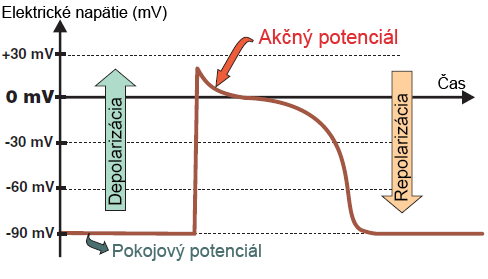
\includegraphics[scale=0.45]{img/action-potential-voltage.png}
    \caption{Akčný potenciál srdcovej membrány \cite{Blahút_2017}.}
    \label{fig:action_potential_voltage}
\end{figure}


%---------------------------------------------------------------
\section{Elektrokardiografia}
%---------------------------------------------------------------

Proces získavania elektrokardiogramu (EKG) nazývame elektrokardiografia. Práve vyššie uvedený stručný popis anatómie a fungovania ľudského srdca je kľúčový pre správnu interpretáciu vzniku EKG. „Elektrokardiografia je metóda, ktorá zaznamenáva elektrickú aktivitu srdca v~čase. Zmeny v rozdiele elektrického potenciálu, teda napätí, ktoré vznikajú počas depolarizácie a repolarizácie myokardiálnych vlákien, sú zaznamenávané elektródami umiestnenými na povrchu hrudníka a končatinách. Zdrojom týchto elektrických potenciálov sú kontraktilné bunky srdcového svalu (kardiomyocity)."\footnote{Pôvodné znenie: \textit{„Electrocardiography is a method that registers electrical activity against time. The changes in electrical potential difference (voltage) during depolarization and repolarisation of the myocardial fibers are recorded by electrodes positioned on the surface of the chest and on the limb (limb leads). The sources of the electrical potentials are contractile cardiac muscle cells (cardiomyocytes)."}} \cite{Wasilewski2011}

V tejto práci sa budeme venovať najmä záťažovej elektrokardiografii, teda ~\textbf{ergometrii}. Aj keď princíp zaznamenávania EKG je ten istý, toto vyšetrenie so sebou nesie určité špecifiká, hlavne ak je vykonávané v teréne. Keďže sa zaznamenáva srdečná aktivita pri fyzickej činnosti, nie je možné, aby mala na sebe sledovaná osoba štandardne umiestnené elektródy. Často musí byť použitý aj iný druh elektród, k tomu sa ale bližšie dostaneme v nasledujúcej časti práce.

\newpage

Vykresľovanie aj interpretácia EKG krivky už síce vo väčšine prípadov prebieha pomocou počítačom riadených EKG systémov, avšak tie stále vizuálne napodobňujú klasickú analýzu na milimetrovom papieri, vrátane tlačeného výstupu. Preto sú fyziologické intervaly, najmä v medicínskej literatúre, často uvádzané v milimetroch. Pre technický charakter tejto práce budeme hodnoty popisujúce dĺžku trvania uvádzať v časových jednotkách, najčastejšie milisekundách (ms). Amplitúdu krivky budeme popisovať v jednotkách elektrického napätia, v prípade EKG konkrétne v milivoltoch (mV). 

%---------------------------------------------------------------
\subsection{Elektródy a zvody}
%---------------------------------------------------------------

Na meranie zmien napätia v srdečnom elektrickom poli sa používajú rôzne druhy elektród, z~hľadiska funkčnosti rozlišujeme pri EKG dva druhy. \textbf{Aktívne elektródy} merajú meniaci sa elektrický potenciál na mieste, na ktorom sú umiestnené. Druhým typom sú \textbf{referenčné alebo nulové elektródy}, ktoré udržiavajú stabilný potenciál, zvyčajne nulový. Spojením dvoch elektród vzniká \textbf{zvod} - imaginárna línia pozdĺž ktorej je meraný elektrický signál. Zvody klasifikujeme na \textbf{bipolárne} a \textbf{unipolárne}. Bipolárne zvody sa skladajú z dvoch aktívnych elektród, zatiaľ čo unipolárne zvody z jednej aktívnej elektródy a jednej nulovej. Pri elektrokardiografickom vyšetrení vykonávanom v ambulancii sa EKG zaznamenáva pomocou štandardizovaného 12-zvodového systému, ktorý má predpísané rozloženie elektród.

%---------------------------------------------------------------
\subsection{Einthovenove končatinové zvody}
%---------------------------------------------------------------

Prvé tri zvody využívané pri 12-zvodovom EKG sú Einthovenove končatinové zvody. Ide o bipolárne zvody, na získanie ktorých potrebujeme 4 elektródy - na ľavej hornej končatine (ĽR), pravej hornej končatine (PR), ľavej dolnej končatine (ĽN) a pravej dolnej končatine (PN). Elektróda na pravej dolnej končatine je nulová, ostatné sú aktívne. Tieto elektródy sa zvyčajne umiestňujú na predlaktie a predkolenie, na presnom umiestnení nezáleží, je však potrebné zabezpečiť vzdialenosť minimálne 10 centimetrov od srdca \cite{garcia201512}.

\noindent Zvody, ktoré vzniknú spojením týchto elektród, označujeme rímskymi číslicami.

\begin{itemize}
    \item \textbf{I. štandardný zvod} - získame ho ako rozdiel potenciálov medzi elektródami na ľavom a~pravom predlaktí.
    \item \textbf{II. štandardný zvod} - 
    získame ho ako rozdiel potenciálov medzi elektródami na pravom predlaktí a ľavom predkolení.
    \item \textbf{III. štandardný zvod} - 
     získame ho ako rozdiel potenciálov medzi elektródami na ľavom predlaktí a ľavom predkolení \cite{Bada2010}.
\end{itemize}

„Štandardné končatinové zvody snímajú srdcové potenciály vo frontálnej rovine. Spojením troch štandardných zvodov vzniká \textbf{rovnostranný Einthovenov trojuholník}, v ktorého približnom strede sa nachádza srdce - v polohe ako sa nachádza v hrudníku." \cite{Bada2010} Tento trojuholník sa používa aj na určenie elektrickej osi srdečnej, ktorou sa ešte budeme zaoberať neskôr v práci.

\begin{figure}[H]
    \centering
    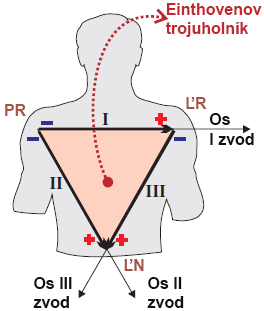
\includegraphics[scale=0.50]{img/einthoven-triangle.png}
    \caption{Einthovenove končatinové zvody \cite{Blahút_2017a}.}
    \label{fig:einthoven}
\end{figure}

%---------------------------------------------------------------
\subsection{Goldbergove končatinové zvody}
%---------------------------------------------------------------

Goldbergove končatinové zvody sú opäť tri, v tomto prípade ale unipolárne - každý je kombináciou jednej aktívnej a jednej nulovej elektródy. Na ich získanie sa využívajú potenciály z~tých istých elektród ako pri Einthovenových zvodoch. Nulová elektróda sa získava prepojením ostatných dvoch, čím sa potenciál aktívnej elektródy umelo zvýši. Od tejto skutočnosti je odvodený aj~pojem \textbf{augmentovaný zvod} a značenie \textbf{aV} (\textit{a = augmented = zvýšené} a \textit{V = voltage = napätie}). Tretie písmeno za skratkou aV značí pozíciu aktívnej elektródy.

\begin{itemize}
    \item \textbf{aVR} - aktívna elektróda je umiestnená na pravom predlaktí, záznam je prevráteným obrazom I. štandardného zvodu.
    \item \textbf{aVL} - aktívna elektróda je umiestnená na ľavom predlaktí, záznam pri tomto zvode sa podobá na I. štandardný zvod.
    \item \textbf{aVF} - aktívna elektróda je umiestnená na ľavom predkolení, záznam pri tomto zvode sa~podobá na III. štandardný zvod \cite{Bada2010}\cite{garcia201512}.
\end{itemize}

\begin{figure}[H]
    \centering
    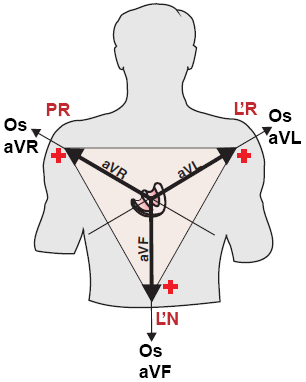
\includegraphics[scale=0.48]{img/goldberger-leads.png}
    \caption{Goldbergove končatinové zvody \cite{Blahút_2017a}.}
    \label{fig:goldberg}
\end{figure}

%---------------------------------------------------------------
\subsection{Wilsonove hrudné zvody}
%---------------------------------------------------------------

Zvyšných šesť zvodov sa nachádza na hrudníku, všetky sú unipolárne a označujú sa V1 až~V6. Na~rozdiel od elektród využívaných Einthovenovými a Goldbergovými zvodmi majú tieto elektró-dy exaktne určenú pozíciu, ktorá je definovaná polohou jednotlivých rebier \cite{Bada2010}\cite{garcia201512}. Predpísané polohy jednotlivých elektród nebudeme bližšie rozpisovať, ilustrované sú na obrázku \ref{fig:wilson}.

Hrudné zvody snímajú elektrickú aktivitu srdca v horizontálnej rovine. „Tvar krivky EKG zaznamenaný pomocou unipolárnych hrudných zvodov determinuje vzájomný vzťah polohy snímajúcej elektródy k smeru šírenia sa vzruchu v srdci. Vzruch v srdci sa šíri smerom od~sínusového uzla v pravej predsieni k srdcovému hrotu." \cite{Bada2010}

\begin{figure}[H]
    \centering
    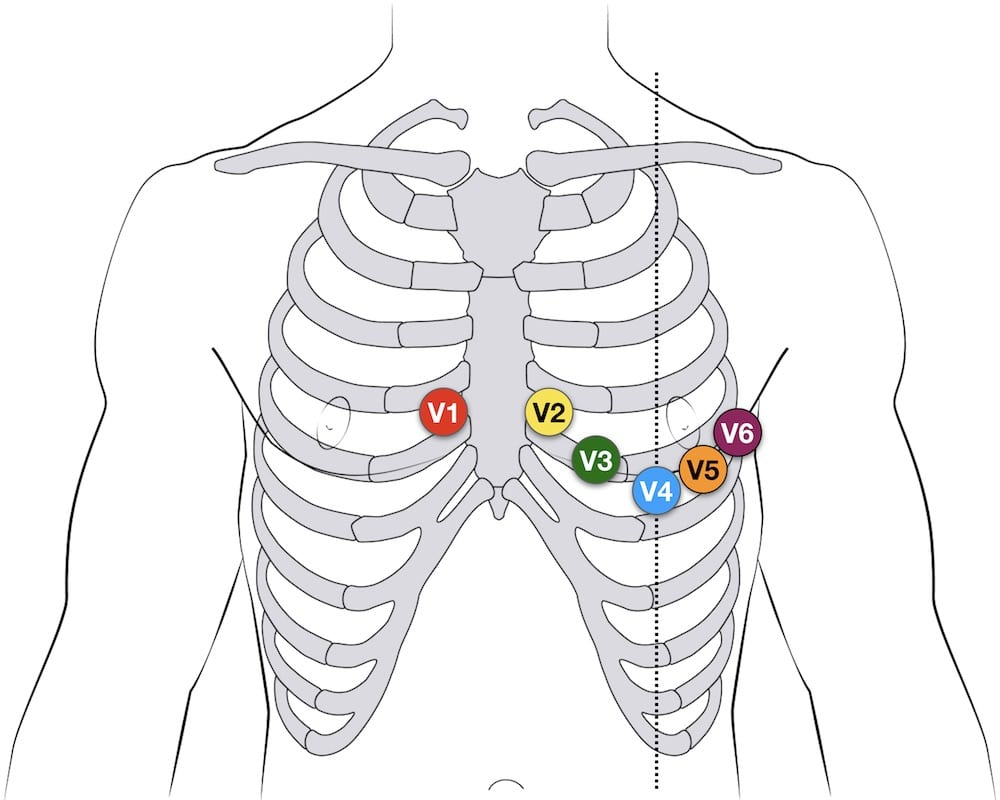
\includegraphics[scale=0.25]{img/12-lead-ECG-lead-placemnet.jpg}
    \caption{Wilsonove hrudné zvody \cite{Cadogan_2022}.}
    \label{fig:wilson}
\end{figure}

Dôležité je spomenúť, že pri dlhodobom terénnom monitorovaní sa často využíva 1-zvodový systém, na ktorý sú potrebné iba dve alebo tri elektródy. Tie sú často umiestnené práve na hrudníku - prvá elektróda na jednom z miest V1 až V6, druhá zrkadlovo na druhej polovici hrudníka, a tretia pod ich úrovňou, v oblasti brucha. Takýmto spôsobom sa minimalizuje počet použitých elektród a káblov potrebných na ich zapojenie, čo je pri dlhodobom monitorovaní prioritou \cite{Thakor1980}.


%---------------------------------------------------------------
\section{Typy povrchových elektród}
%---------------------------------------------------------------

Elektródy používané v elektrokardiografii vieme rozdeliť na povrchové a hĺbkové elektródy. Povrchové elektródy sa umiestňujú na pokožku, zatiaľ čo hĺbkové elektródy sa aplikujú priamo do~srdečného svalu. Pre účely tejto práce nás budú zaujímať iba povrchové elektródy, hĺbkové majú svoje miesto v medicíne najmä pri operatívnych zákrokoch. 

Použitie vhodného typu povrchových elektród je rozhodujúce pre kvalitu výsledného EKG záznamu, pričom rôzne situácie si vyžadujú rôzne druhy elektród. „Keďže EKG je záznam bio elektrických potenciálov na povrchu tela, rozhranie medzi kožou pacienta a elektródami zaznamenávajúcimi EKG je kritické. Významná časť artefaktov zavedených do EKG záznamov sa vyskytuje práve na tomto rozhraní a je spôsobená buď neadekvátnou prípravou kože, alebo nedostatočným kontaktom medzi kožou a elektródou."\footnote{Pôvodné znenie: \textit{„As the ECG is a recording of bioelectrical potentials made at the body surface, the interface between the patient’s skin and the recording electrodes of the ECG is critical. Much of the artifact introduced into ECG recordings occurs at this junction and is caused by inadequate skin preparation or in- adequate skin–electrode contact."}} \cite{Garvey2006} V nasledujúcej časti si predstavíme dva bežné typy povrchových elektród, so zameraním na záťažovú terénnu elektrokardiografiu.

%---------------------------------------------------------------
\subsection{Argentchloridové elektródy}
%---------------------------------------------------------------

Súčasne najpoužívanejším druhom elektród v medicíne sú argentchloridové elektródy, skráte-ne Ag/AgCl elektródy. „Ich názov pochádza od chloridu strieborného AgCl - argentchloridu, sú~základom nie len referenčných elektród pre najrôznejšie analytické systémy, ale zároveň zákla-dom väčšiny elektród určených pre snímanie biologických signálov na povrchu tela." \cite{Roubík2007} Kovová časť tejto elektródy sa skladá zo striebra, na povrchu ktorého je vrstva chloridu strieborného. Ako~elektrolyt, teda materiál ktorý zabezpečí vedenie elektrického prúdu, sa pri týchto elektródach v~medicíne používa fyziologický roztok \cite{Roubík2007}. V tejto kapitole sa vzhľadom na zameranie na dlhodobé terénne monitorovanie budeme venovať iba jednorazovým lepiacim Ag/AgCl elektródam. Pre~úplnosť však spomenieme, že sa v klinickej praxi vyskytujú aj plošné opakovane použiteľné, tie sa však kvôli nutnosti prípravy pokožky vodivým gélom a masívnej konštrukcii na dlhodobé monitorovanie vôbec nepoužívajú.

Jednou z výhod Ag/AgCl elektród je nízka impedancia, teda kladenie minimálneho odporu elektrickému prúdu, kvôli čomu je signál zachytený týmito elektródami dostatočne presný. Ďalšou dôležitou výhodou je pevný kontakt s kožou pacienta, ktorý zaručuje spoľahlivý prenos elektrického signálu aj pri pohybe. Tieto elektródy majú aj nevýhody, ktoré sú najvýznamnejšie práve pri terénnom a dlhodobom monitorovaní. Bežná Ag/AgCl elektróda je určená len na~jedno použitie a odporučená doba skladovania je menej ako jeden rok, po odlepení, či vypršaní doby skladovania, prichádza o svoje pozitívne vlastnosti \cite{Marozas2011}. „Dlhodobé monitorovanie pomocou týchto elektród nie je vhodné, lebo bunky stratum corneum (vonkajšej vrstvy kože) sa v priebehu 24 hodín regenerujú a abrazívny efekt zmizne. Dráždenie pokožky je navyše nepríjemné a~ak~sú~elektródy použité v kombinácii s gélmi, riziko podráždenia pokožky výrazne stúpa. V neposlednom rade ide aj o nepohodlie súvisiace s osobnou hygienou, keďže s nalepenými elektródami sprchovanie nie je možné."\footnote{Pôvodné znenie: \textit{„This measure is not suitable for long-term monitoring because the cells of stratum corneum (outermost layer of the skin) regenerate from deeper skin layers during 24 hours, and the abrasion effect disappears; also, skin abrasion is unpleasant and, if used together with gels, significantly increases the risk of skin irritation. Finally, there is also the personal inconvenience of not being able to shower or bathe while using the electrodes."}} \cite{Marozas2011}

%---------------------------------------------------------------
\subsection{Textilné elektródy}
%---------------------------------------------------------------

Za posledné roky dostupnosť inteligentných nositeľných zariadení rapídne rastie, spolu s čím~výra-zne napreduje aj výskum v oblasti využitia textilných elektród. Tie nie sú primárne určené na~ambulantné monitorovanie, ale na terénne monitorovanie pri stresových a fyzicky náročných profesiách, akými sú zásahové zložky, prípadne na voľnočasové monitorovanie pri športových aktivitách. Textilné elektródy sú väčšinou integrované do oblečenia, alebo do hrudného pásu, a~štandardne sa využíva 1-zvodový EKG systém s dvoma elektródami \cite{Thakor1980}. „Potenciálnou výhodou suchých elektród integrovaných do textilu je to, že sú flexibilné (kvôli čomu sú schopné lepšiemu prispôsobeniu sa telu ako plošné pevné elektródy) a umývateľné, takže sú znovu použiteľné. Táto~vlastnosť znižuje množstvo spotrebného materiálu potrebného na dlhodobé monitorovanie, ktoré je nevyhnutné v prevádzkových prostrediach akými sú vojenské alebo vesmírne operácie."\footnote{Pôvodné znenie: \textit{„The potential advantage of dry electrodes that are textile integrated is that they are both flexible (making them more conformal to the body than traditional rigid disk electrodes) and washable, so it is feasible to use and reuse them. This reduces the consumables required to conduct long-term health monitoring, which is essential for applications in operational environments such as military and space operations."}}~\cite{Arquilla2020}

V literatúre sa najčastejšie opisujú tri rôzne metódy výroby textilných elektród, všetky zdieľajú myšlienku využitia vodivých vlákien, alebo povlakov, na dosiahnutie prenosu elektrického signálu. Vodivé vlákna a povlaky obsahujú kovové častice ako napríklad striebro, uhlík, alebo grafén, v prípade prefabrikovaných tkanín ide o štandardné materiály ako nylon alebo polyester, potiahnuté tenkou vrstvou striebra, prípadne iného kovu \cite{Pani2018}. Prvou metódou je využitie prefabrikovaných textilných tkanív, ktoré sú prišité na odev z vnútornej strany \cite{Vojtech2013}. Výhodou tejto metódy je, že spomedzi spomínaných metód je najmenej prácna, ale zároveň neposkytuje takú flexibilitu pri návrhu dizajnu ako nasledujúce dve metódy. Ďalšou metódou je využitie vodivých vlákien, ktorými sa následne na odev za pomoci tkania alebo pletenia vyšíva požadovaný vzor \cite{Marozas2011}\cite{Fobelets2023}. Výhodou je možnosť vytvorenia hustejšej vrstvy vodivého materiálu \cite{Arquilla2020}. Poslednou možnosťou je využitie vodivých farieb alebo povlakov, ktoré sú pomocou sieťotlače, alebo inej techniky, tlačené na odev. Tento postup dosahuje dobré výsledky, ale je výrazne drahší a~komplikovanejší na výrobu ako predošlé dva \cite{Xu2020}\cite{Paul2015}.

Zvýšenie komfortu monitorovania pri zachovaní dostatočnej spoľahlivosti a presnosti snímania EKG je hlavným cieľom výskumu v oblasti textilných elektród. Tie sú schopné eliminovať mnohé nevýhody spojené s tradičnými Ag/AgCl elektródami, ako dráždenie pokožky, či~vysychanie elektród \cite{Arquilla2020}. Nevýhodou oproti lepiacim argentchloridovým elektródam, a zároveň aj najväčšou výzvou, je zabezpečenie dostatočného kontaktu medzi kožou a elektródou, čo môže predstavovať problém pri pohybe a s ním spojeným potením. „Meniaca sa vzdialenosť a trenie, ktoré sú spôsobené pohybom tela voči povrchu elektródy, sú~hlavným zdrojom chýb - takzvaných pohybových artefaktov."\footnote{Pôvodné znenie: \textit{„Varying distance and friction between the electrode, caused by the movements of the body and surface of an object, are forming a major source of error—so-called motion artifact."}} \cite{Metshein2021}


%---------------------------------------------------------------
\section{EKG krivka}
%---------------------------------------------------------------

V nasledujúcej časti práce popíšeme jednotlivé časti EKG krivky, ktoré sú charakteristické pre~jej~fyziologický priebeh. \textbf{Izoelektrická línia}, alebo čiara, je základom pre každé meranie. Reprezentuje časť signálu, kedy je stav srdca polarizovaný. V EKG zázname ide o rovnú horizontálnu líniu, ktorá slúži ako referenčná hladina k interpretácii jednotlivých vĺn.

%---------------------------------------------------------------
\subsection{Genéza signálu}
%---------------------------------------------------------------

Pri depolarizácii a repolarizácii svalových vlákien dochádza k zmene napätia. To sa na EKG krivke prejavuje ako vlny s rôznou polaritou, ktorá závisí od smeru elektrickej aktivity relatívne k~zvodu. „Vlny, ktoré sa nachádzajú nad úrovňou izoelektrickej čiary, označujeme ako \textbf{pozitívne}, tie, ktoré sú pod jej úrovňou ako \textbf{negatívne}. Vlny, ktorých jedna časť je pozitívna, druhá negatívna, sú \textbf{dvojfázové}." \cite{Bada2010} V EKG krivke pozorujeme P-vlnu, Q-vlnu, R-vlnu, S-vlnu a T-vlnu, ktoré sa typicky nachádzajú v zázname práve v tomto poradí. U zhruba jednej štvrtiny populácie je viditeľná aj šiesta U-vlna, kvôli jej nízkej amplitúde to však nie je pravidlom \cite{Wasilewski2011}. Na obrázku \ref{fig:action_potential_duration} je možné vidieť vzťah medzi akčným potenciálom srdcovej membrány a genézou EKG krivky.

\begin{figure}[H]
    \centering
    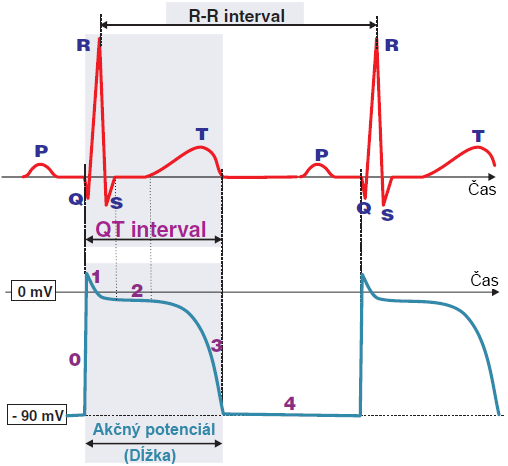
\includegraphics[scale=0.45]{img/action-potential-duration.png}
    \caption{Súvis akčného potenciálu srdcovej membrány a EKG krivky \cite{Blahút_2017}.}
    \label{fig:action_potential_duration}
\end{figure}

\begin{itemize}
    \item \textbf{P-vlna} vzniká pri depolarizácii predsiení. Keďže svalová hmota predsiení je relatívne malá, na EKG krivke pri príslušných zvodoch pozorujeme malú oblú pozitívnu vlnu.
    \item \textbf{QRS komplex}, nazývaný aj komorový komplex, reprezentuje depolarizáciu komôr, obsahuje tri ostré za sebou idúce vlny. Z dôvodu väčšej svalovej hmoty je amplitúda vĺn komplexu výrazne vyššia. 
    \item \textbf{T-vlna} vzniká pri repolarizácii komôr, podobne ako pri P-vlne ide o malú oblú pozitívnu vlnu \cite{Foster_2007}\cite{Bada2010}.
\end{itemize}

%---------------------------------------------------------------
\subsection{Elektrická os srdečná}
%---------------------------------------------------------------

Aktivita srdca sa dá popísať mnohými vektormi, ktoré reprezentujú smer a silu elektrickej aktivity vznikajúcej v srdci. Samostatne vieme určiť napríklad aj elektrickú os srdcových komôr, pomocou vektorovej aritmetiky. „Konečný vektor, po všetkých sčítaniach, odčítaniach a zmenách smeru, reprezentuje elektrickú os srdcovej komory. Rovnako má každá vlna a každý segment tiež svoj príslušný vektor, vektor P-vlny, vektor S-T segmentu, alebo QRS vektor. EKG zachytáva tieto vektory počas toho, ako prechádzajú pod elektródou."\footnote{Pôvodné znenie: \textit{„That final vector, after all of the addition, subtraction, and direction changes, is known as the electrical axis of the ventricle. In the same way, each wave and segment has its own respective vector. There is a P-wave vector, a T-wave vector, an ST segment vector, and a QRS vector. The ECG is a measurement of these vectors as they pass under an electrode."}} \cite{garcia201512}

Amplitúda vlny zobrazenej na EKG krivke závisí od uhlu, ktorý zviera vektor elektrického impulzu so zvodom. Ak je vektor paralelný s osou zvodu, amplitúda bude pri danom zvode maximálna, a klesá spolu s narastajúcim uhlom medzi nimi. V prípade, že sú na seba kolmé, na EKG krivke je viditeľná izoelektrická línia. Od orientácie vektoru elektrického impulzu zase záleží, či bude vlna na EKG krivke zobrazená ako pozitívna, alebo negatívna. 
 
\begin{itemize}
    \item \textbf{Pozitívna vlna} vzniká, ak sa pozitívny impulz hýbe smerom k elektróde. Keďže výsledkom depolarizácie je pozitívny potenciál, ak sa depolarizácia hýbe smerom k elektróde, vzniká pozitívna vlna. Opak platí pre repolarizáciu, pri ktorej vzniká negatívny potenciál - vlna bude pozitívna, ak sa hýbe smerom od elektródy.
    \item \textbf{Negatívna vlna} vzniká, ak sa pozitívny impulz hýbe smerom od elektródy. Z tvrdenia vyššie vyplýva, že ak sa depolarizácia hýbe v smere od elektródy, zaznamenaná vlna bude negatívna, a analogicky platí to isté, keď sa repolarizácia hýbe smerom od elektródy \cite{garcia201512}\cite{Euan_Niebauer_2004}.
\end{itemize}

\begin{figure}[H]
    \centering
    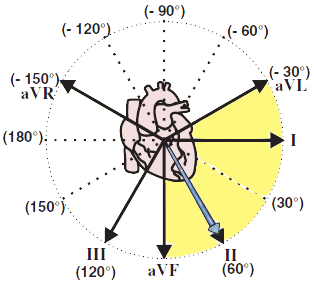
\includegraphics[scale=0.6]{img/normal-axis.png}
    \caption{Elektrická os srdečná \cite{Blahút_2017b}.}
    \label{fig:axis}
\end{figure}

Fyziologicky je elektrická os srdečná orientovaná medzi -30° až + 90°, teda v ľavom dolnom kvadrante, ako je možné vidieť na obrázku \ref{fig:axis}. Keďže sa elektrický impulz v srdci šíri od pravej predsiene smerom k srdcovému hrotu, fyziologicky os približne zodpovedá orientácii srdca v hrudnej dutine \cite{Bada2010}. V prípade patológie označujeme elektrickú os ako derivovanú doprava, alebo derivovanú doľava.

%---------------------------------------------------------------
\subsection{Interpretácia EKG}
%---------------------------------------------------------------

Elektrokardiogram je kvôli dostupnosti a neinvazívnemu charakteru tejto metódy najčastejšie využívaná metóda v kardiológii. Dôkladnou analýzou záznamu je možné diagnostikovať rôzne srdcovo-cievne ochorenia, ako napríklad arytmie, či infarkt myokardu. Najdlhšou súvisle interpretovanou časťou v EKG krivke je QRS komplex, ktorý je tvorený zhlukom troch rovnomenných vĺn. Okrem samotných vĺn v rámci EKG krivky interpretujeme aj trvanie dvoch základných charakteristík - segmentov a intervalov.
\begin{itemize}
    \item \textbf{Segment} je časť izoelektrickej línie medzi jednotlivými vlnami, interpretujeme napríklad S-T alebo P-R segment.
    \item \textbf{Interval} je ohraničený začiatkom jednej a začiatkom druhej vlny. Tieto vlny môžu byť buď~z~toho istého srdečného cyklu, ako napríklad P-R alebo Q-T interval, alebo z dvoch po sebe idúcich cyklov, ako v prípade R-R intervalu \cite{Wasilewski2011}.
\end{itemize}

\newpage

Pri interpretácii EKG sa kladie dôraz na dobu trvania a amplitúdy jednotlivých vĺn, segmentov, aj intervalov, pričom namerané hodnoty sa porovnávajú s fyziologickými. V tejto práci sa diagnostike srdcovo-cievnych ochorení venovať nebudeme, avšak v odbornej literatúre je~možné nájsť veľké množstvo relevantných informácií k tejto téme \cite{Wasilewski2011}\cite{Bada2010}\cite{Foster_2007}.


%---------------------------------------------------------------
\section{Artefakty v EKG}
%---------------------------------------------------------------

Artefakty sú definované ako nežiaduce signály, alebo interferencie, ktoré nesúvisia s elektrickou aktivitou srdca a môžu viesť k nesprávnej interpretácii skutočného EKG signálu. Pochádzajú z~rôznych zdrojov fyziologického, technického, alebo environmentálneho pôvodu. Keď sú artefakty superponované na EKG signáli, izoelektrická línia alebo jednotlivé vlny pôsobia skreslené, čo~môže viesť k nesprávnej diagnostike. Niektoré artefakty môžu svojim vzhľadom napodobňovať klinicky významné arytmie, ako napríklad fibriláciu predsiení alebo komorovú tachykardiu. Veľkú časť týchto artefaktov nie je možné odstrániť bez straty dôležitej informácie. 

Jedným z možných zdrojov artefaktov je chybné zapojenie elektród. Artefaktom tohto pôvodu sa ďalej nebudeme venovať, iba pre úplnosť spomenieme, že môžu spôsobiť prevrátený alebo inverzný signál pri postihnutých zvodoch \cite{PrezRiera2017}\cite{Littmann2021}. V nasledujúcej časti práce si popíšeme artefakty, so zameraním na tie spôsobené fyzickou činnosťou. Príklad EKG krivky, na ktorej je zaznamenaný fyziologický \textbf{sínusový rytmus}, bez znečistenia artefaktmi, je~možné vidieť na~obrázku \ref{fig:sinus}.

\begin{figure}[H]
    \centering
    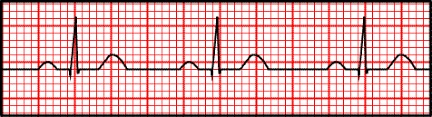
\includegraphics[scale=0.72]{img/sinus.jpg}
    \caption{Sínusový rytmus \cite{Mauvila_2018}.}
    \label{fig:sinus}
\end{figure}

%---------------------------------------------------------------
\subsection{Kolísanie izoelektrickej línie}
%---------------------------------------------------------------

\begin{figure}[H]
    \centering
    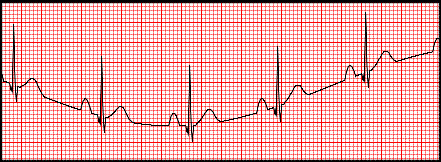
\includegraphics[scale=0.7]{img/baseline.jpg}
    \caption{Kolísanie izoelektrickej línie \cite{Mauvila_2018}.}
\end{figure}

Ide o nízkofrekvenčný artefakt prejavujúci sa v EKG signáli ako postupný posun izoelektrickej línie v čase. Kolísanie izolínie môže pochádzať z rôznych zdrojov, často ide o respiračný artefakt spôsobený pohybom hrudníka pri dýchaní. Nedostatočný kontakt elektródy s kožou, prípadne nesúlad impedancií, môže spôsobiť kolísanie keď elektrický signál narazí na odpor na~rozhraní koža-elektróda. Častým zdrojom je aj mimovoľný pohyb elektród spôsobený nedostatočnou fixáciou ku koži \cite{Romero2018}. 

Špecifickým druhom kolísania izoelektrickej línie je takzvaný \textbf{abrupt}, ktorý je charakteristický rýchlym preskokom. Tento druh kolísania úzko súvisí s pohybovými artefaktmi, keďže je často spôsobený dotykom elektródy, a je ťažké ho odstrániť bez straty informácie.

Medzi najpoužívanejšie metódy odstránenia kolísajúcej izolínie patria analógové alebo digitálne filtre s konečnou alebo nekonečnou odozvou, ktoré sú schopné selektívne prepúšťať alebo tlmiť špecifické frekvenčné zložky signálu. Analógové filtre sú zabudované priamo v zariadení snímajúcom EKG, kde filtrujú signál ešte pred digitalizáciou. Keďže ide o nízkofrekvenčný artefakt, využívajú sa filtre typu horná priepust, ktoré prepúšťajú frekvencie vyššie ako stanovená hranica a tlmia nižšie. Porovnanie efektívnosti týchto filtrov je možné nájsť v odbornej literatúre, pričom sa kladie dôraz na čo najmenšiu stratu informácie v pôvodnom EKG signáli \cite{Romero2018}\cite{Kaur2011}.

%---------------------------------------------------------------
\subsection{Sieťové rušenie}
%---------------------------------------------------------------

\begin{figure}[H]
    \centering
    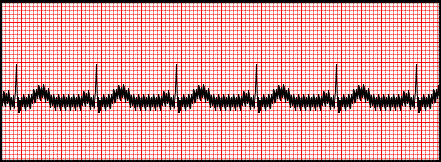
\includegraphics[scale=0.7]{img/acinterference.jpg}
    \caption{Sieťové rušenie \cite{Mauvila_2018}.}
\end{figure}

Zdrojom sieťového rušenia je striedavý prúd. Ide o rušenie s frekvenciou 50 Hz\footnote{Na území Európy sa štandardne elektrické zariadenia napájajú na striedavý prúd s frekvenciou 50 Hz, v iných častiach sveta je to často 60 Hz.}, ktoré sa prejavuje ako periodické fluktuácie v podobe špičiek superponovaných na skutočnej EKG krivke. Tento artefakt môže vznikať ako dôsledok elektromagnetickej väzby medzi elektrickými zvodmi, prípadne v dôsledku nedostatočného uzemnenia \cite{Huhta1973}. „Prítomnosť iných elektrických zariadení v~miestnosti, kde sa zaznamenáva EKG, môže spôsobiť záznamy s viditeľným elektrickým rušením. V~týchto prípadoch by mali byť všetky zariadenia, ktoré môžu rušiť EKG signál, vypnuté. Medzi takéto zariadenia patria mobilné telefóny vo vzdialenosti menšej ako 25 cm od zariadenia zaznamenávajúceho EKG, elektrické lôžka, či chirurgické alebo fluorescenčné lampy."\footnote{Pôvodné znenie: \textit{„The presence of other electrical devices in the room where the ECG is being conducted may cause recordings with electrical inter- ference. In such cases, any device that may interfere with the ECG signal should be turned off: these include cell phones within 25 cm of the ECG sensor module, electrical beds, surgical and fluorescent lamps."}} \cite{PrezRiera2017}

Zabezpečenie správneho uzemnenia EKG zariadenia a tienenia káblov pred elektromagnetickým rušením znižuje pravdepodobnosť výskytu artefaktov. Navyše majú systémy na~monitorovanie EKG v sebe často integrované analógové filtre, ktoré tento artefakt potláčajú. Keďže ide~o~opakované rušenie so známou frekvenciou, najčastejšie sa využívajú na jeho filtráciu hrebe-ňové filtre\footnote{Často v literatúre uvádzané aj v pôvodnom anglickom znení ako \textit{notch filtre.}}, ktoré sú schopné potláčať konkrétne frekvencie, prípadne iné varianty pásmovej zádrže, ako napríklad Butterworthov filter \cite{Gilani2018}.

%---------------------------------------------------------------
\subsection{Pohybové artefakty}
%---------------------------------------------------------------

\begin{figure}[H]
    \centering
    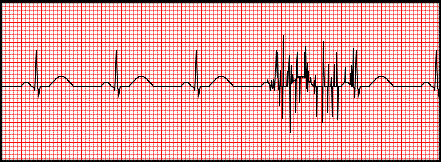
\includegraphics[scale=0.7]{img/tremor.jpg}
    \caption{Pohybový artefakt \cite{Mauvila_2018}.}
\end{figure}

Pohybové artefakty sú najväčším problémom pri záťažovom testovaní. Zdrojom týchto artefaktov sú samotné nárazy spôsobené pohybom, zmena kontaktu medzi kožou a elektródou, či zmena impedancie na rozhraní koža-elektróda \cite{Kirst2011}. Špecifickým typom pohybového artefaktu sú \textbf{myopotenciály}, ktoré vznikajú kvôli svalovým kontrakciám.

Odstránenie pohybových artefaktov je najväčšou výzvou spomedzi spomínaných EKG artefaktov. Dôvodom je, že frekvenčné spektrum týchto artefaktov sa do významnej miery prekrýva so spektrom EKG, takže odstránenie bez straty dôležitej informácie nie je možné \cite{Li2020}. Aj~keď toto tvrdenie platí do istej miery pre väčšinu vyššie uvedených artefaktov, pri~nízkofre-kvenčnom kolísaní izoelektrickej línie je vplyv filtrácie minimálny, to isté platí aj pri sieťovom rušení, keďže je úzkopásmové a dá sa tak číslicovo filtrovať. Významný problém nastáva pri~fil-trácii abruptov, tie však môžeme z hľadiska pôvodu radiť medzi pohybové artefakty. „Pohybové artefakty môžu produkovať signály s veľkou amplitúdou, ktoré pripomínajú P-vlny, T-vlny, či~QRS-komplex. Sú prítomné počas ambulantného monitorovania a záťažových testov. Z klinického hľadiska môžu viesť k stanoveniu nesprávnej diagnózy, alebo oneskoreným či nevhodným rozhodnutiam týkajúcich sa liečby. Efektívne potlačenie pohybového artefaktu je v~klinickom prostredí zatiaľ nevyriešeným problémom."\footnote{Pôvodné znenie: \textit{„Motion artifact can produce large amplitude signals in the ECG and can resemble the P, QRS, and T waveforms of the ECG. Motion artifact is prevalent during ambulatory monitoring and treadmill stress testing. From the clinical standpoint, motion artifact can result in misdiagnosis and may lead to delayed or inappropriate treatment decisions. Effective reduction of motion artifact is an unsolved problem in the clinical setting."}} \cite{Tong} 

Existujú postupy, ktorými sa dajú pohybové artefakty potlačiť, napríklad adaptívnou filtráciou, kedy sa parametre filtru dynamicky menia \cite{Kirst2011}\cite{Tong}, tieto riešenia však často nie sú~dostatočné. V tejto práci sa nebudeme zaoberať filtráciou pohybových artefaktov, ale ich automatickou detekciou. Pri dlhodobom terénnom monitorovaní je žiadúce tieto úseky identifikovať a~následne od nich signál očistiť - segmenty znečistené pohybovými artefaktami zahodiť.


%---------------------------------------------------------------
\section{Automatická detekcia artefaktov v EKG}
%---------------------------------------------------------------

Problém detekcie pohybových artefaktov je vo svojej podstate problémom detekcie anomálií. V~našom prípade anomálie nebudú predstavovať poruchy srdcového rytmu, ani iné z diagnostického hľadiska patologické javy čitateľné z EKG krivky, ale samotné artefakty. Na rozdiel od~detekcie anomálií sa detekcia pohybových artefaktov nezaoberá iba identifikáciou nesprávnych vzorov či deviácií od stanovenej normy, ale zaoberá sa aj posudzovaním kvality signálu.\footnote{Tento problém je v anglickej literatúre možné nájsť pod pojmom \textit{signal quality assessment} (SQA).} Práve kvalita signálu je rozhodujúca pri ďalšom spracovaní a interpretácii EKG záznamu.

Všetky z uvedených artefaktov sú ľahko identifikovateľné pomocou vizuálnej inšpekcie, zaujímavým aspektom tohto problému je však \textit{automatická} detekcia, s ktorou majú tradičné metódy spracovania signálu problém. Práve to, že tradičné metódy na automatickú detekciu pohybových artefaktov nestačia, je motiváciou skúmať v tejto práci metódy založené na umelej inteligencii.

%---------------------------------------------------------------
\subsection{Tradičné metódy spracovania signálu}
%---------------------------------------------------------------

Medzi tradičné metódy spracovania signálu budeme radiť metódy zaoberajúce sa štatistickou analýzou a rôzne techniky dekompozície signálu. Patrila by sem aj analógová a~digitálna filtrácia, ale kvôli prekrývajúcemu sa frekvenčnému spektru tento prístup nie je v prípade pohybových artefaktov účinný. V krátkosti uvedieme dve metódy tradičného spracovania signálov vyskytujúce sa v literatúre v kontexte posudzovania kvality signálu a detekcie artefaktov.

\begin{itemize}
    \item \textbf{Analýza nezávislých komponentov (ICA)} je metóda dekompozície signálu, ktorá dokáže rozložiť signál na množinu štatisticky nezávislých komponentov, predpokladom je, že dáta pochádzajú z iného ako Gaussovského rozdelenia. Tým, že pohybové artefakty a EKG signál pochádzajú zo štatisticky nezávislých zdrojov, táto metóda je schopná ich odseparovať \cite{Milanesi2007}.
    \item \textbf{Vlnková transformácia} funguje na podobnom princípe ako Fourierova transformácia, ale je~vhodnejšia na detekciu pohybových artefaktov. Nerozkladá signál iba na harmonické zložky, ktoré pretrvávajú po celú dobu signálu, ale dokáže nájsť zložky definované špecifickou frekvenciou a časom. Analýzou získaných vlnkových koeficientov sa dajú odhaliť časovo-frekvenčné charakteristiky pohybového signálu \cite{Bhoraniya2014}.
\end{itemize}

Nevýhodou použitia tradičných metód je, že sa často spoliehajú na analýzu špecifických charakteristík vstupných dát. Kvôli tomu nie sú schopné dobre generalizovať naprieč rôznymi množinami dát, ktoré napríklad nemusia byť zaznamenané za tých istých podmienok. Toto predstavuje problém, keďže pohybové artefakty sú veľmi variabilné, závisia od vykonávanej aktivity, ale aj od polohy a typu elektród. Ďalšou významnou nevýhodou je časová náročnosť výpočtu. Metódy umelej inteligencie sú typicky vo fáze učenia tiež časovo náročné, avšak pri predikcii už nie. Výhodou tradičných metód je dobrá interpretovateľnosť výsledkov, tá sa však dá lepšie aplikovať na analýzu vlastností pohybových artefaktov, než na samotnú automatickú detekciu.

\newpage

%---------------------------------------------------------------
\subsection{Umelé neurónové siete (ANN)}
%---------------------------------------------------------------

Aby sme mohli ďalej rozoberať konkrétne architektúry neurónových sietí, ktoré sa využívajú na analýzu signálov, alebo časových rád, potrebujeme uviesť krátky opis umelých neurónových sietí ako takých. Sú to výpočtové modely, ktoré svojou štruktúrou pripomínajú ľudský nervový systém, čím sa snažia nadobudnúť schopnosť \textbf{generalizovať} a riešiť komplexné problémy. 

Model neurónu obsahuje \textit{n} vstupov, ktoré značíme \textit{x\textsubscript{1}} až~\textit{x\textsubscript{n}}, k ním prislúchajú váhy \textit{w\textsubscript{1}} až~\textit{w\textsubscript{n}}. Výstup neurónu \textit{y} je definovaný vzorcom \ref{eq:1}, dostávame ho ako lineárnu kombináciu vektoru vstupov \textit{\( \Bar{x} \)} a vektoru váh \textit{\( \Bar{w} \)}. \textit{T} predstavuje prah, pri ktorom je neurón aktivovaný a~\textit{f}~definuje \textbf{aktivačnú funkciu}. 

\begin{equation} 
    \label{eq:1}
    y = f(\sum_{i=0}^{n} w_i x_i - T)
\end{equation}

Tá zavádza do modelu žiadanú nelinearitu, a mala by byť spojitá a diferencovateľná kvôli učeniu pomocou gradientných optimalizačných algoritmov. Častou voľbou vo výstupnej vrstve pri binárnej klasifikácii je \textbf{sigmoida} \ref{eq:2}, pri klasifikácii do viacerých tried funkcia \textbf{softmax} \ref{eq:3}. Softmax narozdiel od sigmoidy dáva na výstup rozdelenie pravdepodobnosti naprieč \textit{K} triedami, pričom zaručuje, že súčet jednotlivých pravdepodobností bude rovný jednej \cite{Zou2008}\cite{yegnanarayana2009artificial}\cite{mehrotra1997elements}.

\vspace{5pt}
\noindent
\begin{minipage}[t]{.45\textwidth}
    \begin{equation} 
        \label{eq:2}
        \sigma(x) = \frac{1}{1 + e^{-x}}
    \end{equation}
\end{minipage}
\hfill
\begin{minipage}[t]{.45\textwidth}
    \begin{equation} 
        \label{eq:3}
        softmax(x_i) = \frac{e^{x_i}}{\sum_{j=1}^{K} e^{x_j}}
    \end{equation}
\end{minipage}
\vspace{5pt}

Z hľadiska prepojenia neurónov poznáme dva rôzne druhy neurónových sietí - \textbf{dopredné a spätnoväzebné}. V dopredných sieťach sa informácia šíri iba jedným smerom, zatiaľ čo v spätnoväzebných sú umožnené aj spätné prepojenia, príkladom sú rekurentné neurónové siete.
Jednotlivé neuróny sú usporiadané do lineárnych polí, tie sa nazývajú \textbf{vrstvy}. Poznáme tri rôzne typy vrstiev z hľadiska usporiadania a to vstupné, skryté a výstupné. 

Optimalizáciu vektorov váh \textit{\( \Bar{w} \)} nazývame \textbf{učenie} neurónovej siete. V skutočnosti ide~o~iteratívne hľadanie minima \textbf{stratovej funkcie}. Na začiatku sú vektory váh inicializované náhodne, prípadne je možné použiť heuristiku. V každej iterácii trénovania, teda \textbf{epoche}, sa~naj-skôr vykoná \textbf{dopredný krok}, kedy sa vstupné dáta propagujú sieťou až na výstup. Následne sa~vypočíta strata modelu, porovnaním predikcií so správnymi hodnotami. Ako stratová funkcia pri klasifikačných úlohách sa často volí \textbf{kategorická krížová entropia}, ktorá je zadefinovaná ako \ref{eq:4}, kde \textit{c} značí počet tried.

\begin{equation} 
    \label{eq:4}
    L = -\sum_{i=1}^{c} y_i log(\hat{y_i})
\end{equation}

Vypočítaná strata modelu sa následne pomocou algoritmu \textbf{spätného šírenia chyby} propaguje neurónovou sieťou späť. Ako posledný krok jednej epochy sa vykoná aktualizácia váh modelu, kedy sa pomocou gradientnej optimalizácie posunú ich hodnoty proti smeru gradientu, teda smerom k minimu funkcie \cite{Zou2008}\cite{yegnanarayana2009artificial}\cite{mehrotra1997elements}. Aktualizácia \textit{n}-tej váhy je definovaná vzťahom \ref{eq:5}, pričom \textit{\( \alpha \)} predstavuje hyperparameter \textbf{learning rate}, ktorý reguluje rýchlosť učenia.

\begin{equation} 
    \label{eq:5}
    *w_n = w_n - \alpha(\frac{\delta L}{\delta w_n})
\end{equation}

Darji a spol.\cite{Darji2013} riešili v svojej publikácii problém podobný nášmu použitím umelých neurónových sietí. Pomocou algoritmu na synchronizáciu R-špičiek a adaptívnej filtrácie odhadli z dát zložku reprezentujúcu pohybový artefakt pri štyroch rôznych fyzických aktivitách. Následne zo získaných zložiek ešte extrahovali časové a frekvenčné príznaky, ktoré potom vložili na vstup umelej neurónovej siete s desiatimi skrytými vrstvami. Na výstupe predikovali typ pohybovej aktivity s presnosťou 89,07 \%. Využitie tohto postupu v reálnom čase však nie je kvôli časovo náročnému predspracovaniu dát možné.

%---------------------------------------------------------------
\subsection{Konvolučné neurónové siete (CNN)}
%---------------------------------------------------------------

Konvolučné neurónové siete sú určené na spracovanie viac-dimenzionálnych dát, akými sú naprí-klad časové rady alebo obrazové dáta. Špeciálne vrstvy vykonávajú operáciu nazývanú konvolúcia, použitý filter sa nazýva \textbf{kernel}. Okno filtra sa postupne posúva cez dáta, pričom počíta jednotlivé skalárne súčiny, ktoré sa zapisujú na príslušnú pozíciu výstupnej matice. Operácia konvolúcie je znázornená na obrázku \ref{fig:convolution}, kde je matica \textit{I} konvolvovaná s kernelom \textit{K}. Okrem toho, že tieto vrstvy umožňujú hirearchickú extrakciu príznakov, slúžia aj na zníženie komplexnosti modelu, keďže nie sú plne prepojené.

\begin{figure}[H]
    \centering
    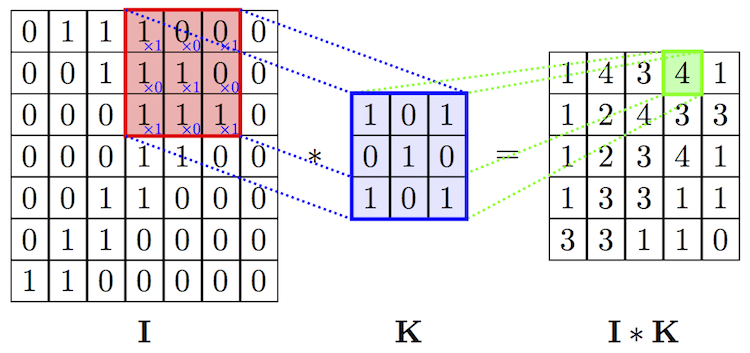
\includegraphics[scale=0.3]{img/convolution.png}
    \caption{Konvolúcia matice s kernelom \cite{mohamed2017}.}
    \label{fig:convolution}
\end{figure}

\noindent Architektúra týchto sietí zahŕňa kombináciu plne prepojených, konvolučných a poolingových vrstiev.
\begin{itemize}
    \item \textbf{Konvolučné vrstvy} sú filtre, ktoré umožňujú neurónovej sieti extrahovať konkrétne informácie. Výsledkom aplikácie konvolúcie na dáta sú matice nazývané \textbf{aktivačné mapy}. Takto získané mapy je možné vizualizovať a analyzovať tak získané príznaky. 
    \item \textbf{Poolingové vrstvy} redukujú rozmer vzniknutých máp, susedné prvky sú zlúčené do jedného, pomocou matematických operácií ako sčítanie, alebo priemerovanie. Tieto vrstvy opäť redukujú komplexnosť siete a znižujú aj riziko preučenia.
    \item \textbf{Plne prepojené vrstvy} sú zodpovedné za integráciu informácií získaných v jednotlivých konvolučných vrstvách a následný výpočet predikcií \cite{Sakib2019}\cite{Aloysius2017}\cite{Albawi2017}.
\end{itemize}

Zhang a spol. \cite{Zhang2019} na klasifikáciu kvality EKG signálu využili kaskádu konvolučných neurónových sietí. Architektúra siete sa skladá z dvoch hlavných pod-sietí. Prvá klasifikuje signál do troch kategórií - pohybový artefakt, myopotenciál a signál s minimálnym rušením. Výstup z~tejto pod-siete následne ide na vstup do druhej, ktorá ďalej klasifikuje pohybové artefakty a~myopotenciály na mierne a závažné. Prvá pod-sieť sa skladá z troch samostatných sietí. Do~jednej siete ide na vstup EKG signál očistený od šumu, do druhej vstupuje spektrogram signálu získaný pomocou krátkodobej Fourierovej transformácie. \\Výstupy z oboch sietí idú na vstup do jedno-vrstvovej neurónovej siete obsahujúcej plne prepojenú vrstvu so softmax aktivačnou funkciou, ktorá výsledok klasifikuje do jednej z troch tried.

Dáta boli získané z II. zvodu 12-zvodového Holter monitoru, pričom dátová sada pozostáva z 90 000 segmentov. Dĺžka jedného segmentu bola zvolená ako 4 sekundy, a segment bol anotovaný podľa dominantného artefaktu. Artefakt bol segmentu priradený v prípade, že~presahoval dĺžku 2 sekundy, závažnosť artefaktu bola odvodená od amplitúdy, relatívne k amplitúde R-špičky. Vyhodnotenie zohľadňuje aj presnosť klasifikácie pri rôznych arytmiách zastúpených v dátovej sade, súhrnná presnosť bola 92,7 \%. Kvôli komplexite získania dát a ich množstvu je~rozsah tejto štúdie neporovnateľný s našou \cite{Zhang2019}.

%---------------------------------------------------------------
\subsection{Rekurentné neurónové siete (RNN)}
%---------------------------------------------------------------

Spätné väzby v RNN umožňujú pamätať si informáciu a modelovať dáta obsahujúce časové závislosti. Pri analýze časových radov to znamená, že sú schopné efektívne riešiť problémy ako~rozpoznávanie vzorov v dátach, či detekciu anomálií. 

Tradičné architektúry rekurentných neurónových sietí sa spoliehajú na spätné prepojenia, príkladom je plne-prepojená RNN, kde je každý neurón v skrytej vrstve napojený na~všetky ostatné neuróny. Spolu s narastajúcou vzdialenosťou strácajú schopnosť pamätať si informáciu, takže nie sú vhodné na modelovanie dlhodobých časových závislostí \cite{Staudemeyer2019}. Druhým problémom je~miznúci gradient, kedy gradient propagovaný cez mnoho časových krokov začne exponenciálne klesať, následkom čoho sa váhy aktualizujú po veľmi malých krokoch, čo vedie k stagnácii trénovania \cite{Hochreiter1998}. 

Riešením oboch problémov je novšia architektúra rekurentných neurónových sietí Long Short-Term Memory (\textbf{LSTM}). Táto architektúra využíva pamäťové LSTM bunky, ktoré majú v~pamäti uložený vektor reprezentujúci ich stav. Tok informácií dnu a von z tejto bunky je~kontrolovaný pomocou brán, ktoré umožňujú zachytávať aj dlhodobé vzťahy v dátach \cite{Yu2019}.

Kvôli nutnosti propagácie chyby cez rekurentné prepojenia použitie štandardného tréno-vacieho algoritmu spätného šírenia chyby nie je možné. Miesto toho sa~najčastejšie využíva jeho rozšírená verzia, nazývaná \textbf{algoritmus spätného šírenia chyby v čase (BPTT).} „Na konci trénovacej sekvencie sa sieť rozvinie v čase a vypočíta sa chyba pre dvojice vstupov a výstupov pomocou zvolenej metriky. Následne sa táto chyba propaguje späť sieťou a vypočíta sa aktualizácia váh pre každý krok v čase. Na záver sa váhy v rekurentnej verzii siete aktualizujú ako súčet vypočítaných zmien naprieč všetkými krokmi."\footnote{Pôvodné znenie: \textit{„At the end of a training sequence, the network is unfolded in time. The error is calculated for the output units with existing target values using some chosen error measure. Then, the error is injected backwards into the network and the weight updates for all time steps calculated. The weights in the recurrent version of the network are updated with the sum of its deltas over all time steps."}} \cite{Yu2019} Ukážka rozvinutia rekurentnej neurónovej siete v čase \textit{t} je na obrázku \ref{fig:backpropagation}.

\begin{figure}[H]
    \centering
    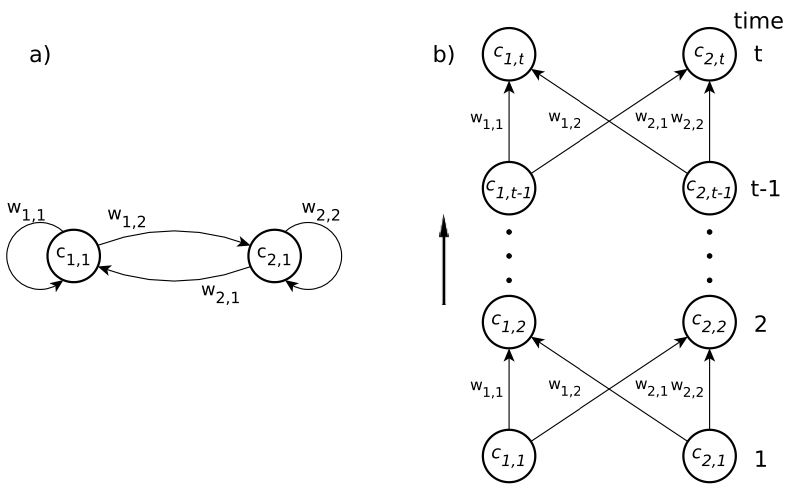
\includegraphics[scale=0.7]{img/backpropagation.png}
    \caption{Rozvinutie rekurentnej neurónovej siete v čase \cite{Yu2019}.}
    \label{fig:backpropagation}
\end{figure}

Boljanić a spol. \cite{boljanic2022} sa v ich publikácii zaoberajú detekciou EKG artefaktov pomocou LSTM neurónových sietí. Dáta, na ktorých bola táto sieť trénovaná, úzko súvisia so zámerom našej práce - EKG signály z 1-zvodového systému boli zaznamenané od horských záchranárov počas zásahu. Signál bol rozdelený na 10 sekundové segmenty, a segment bol označený ako~obsahujúci pohybový artefakt ak viac ako polovica segmentu obsahovala šum, kvôli ktorému sa~nedal jasne detegovať QRS-komplex. Architektúra použitej siete sa skladá z obojsmernej LSTM vrstvy (BiLSTM), ktorej výstup ide na vstup plne prepojenej vrstvy so softmax aktivačnou funkciou. Po vyladení hyperparametrov bola táto architektúra schopná dosiahnuť presnosť 90,1~\% na testovacích dátach. Hlavným obmedzením tohto prístupu je dlhé časové okno.

%---------------------------------------------------------------
\subsection{Support vector machines (SVM)}
%---------------------------------------------------------------

SVM je trieda modelov, ktorá sa najčastejšie používa na klasifikáciu dát. Problém, ktorý tieto modely riešia, je nájdenie \textbf{optimálnej separačnej nadroviny}, ktorá maximalizuje vzdialenosť jednotlivých dátových bodov od nej. V prípade lineárne separovateľných dát je typicky možné nájsť nekonečne mnoho nadrovín separujúcich dáta. SVM operujú s myšlienkou, že čím ďalej dátové body od tejto nadroviny ležia, tým istejšia je klasifikácia, a teda schopnosť modelu generalizovať narastá. Okolo nadroviny sa nachádza pásmo, v ktorom neležia žiadne body, hľadáme teda maximálny okraj\footnote{V anglickom jazyku \textit{maximal margin}.}. Na definovanie nadroviny nám stačia body ležiace na tomto okraji, ktorých je typicky málo, takže sa pri výpočte pracuje s riedkou maticou, kvôli čomu je táto metóda výpočtovo efektívna. Body, na ktorých závisí poloha nadroviny, nazývame \textbf{podporné vektory}\footnote{V anglickom jazyku \textit{support vectors}.}. Na obrázku \ref{fig:margin} hrubá čiara reprezentuje optimálnu separačnú nadrovinu, a \textit{\( \gamma \)} definuje maximálny okraj \cite{Cristianini_Scholkopf_2002}\cite{Suthaharan2016}.

\begin{figure}[H]
    \centering
    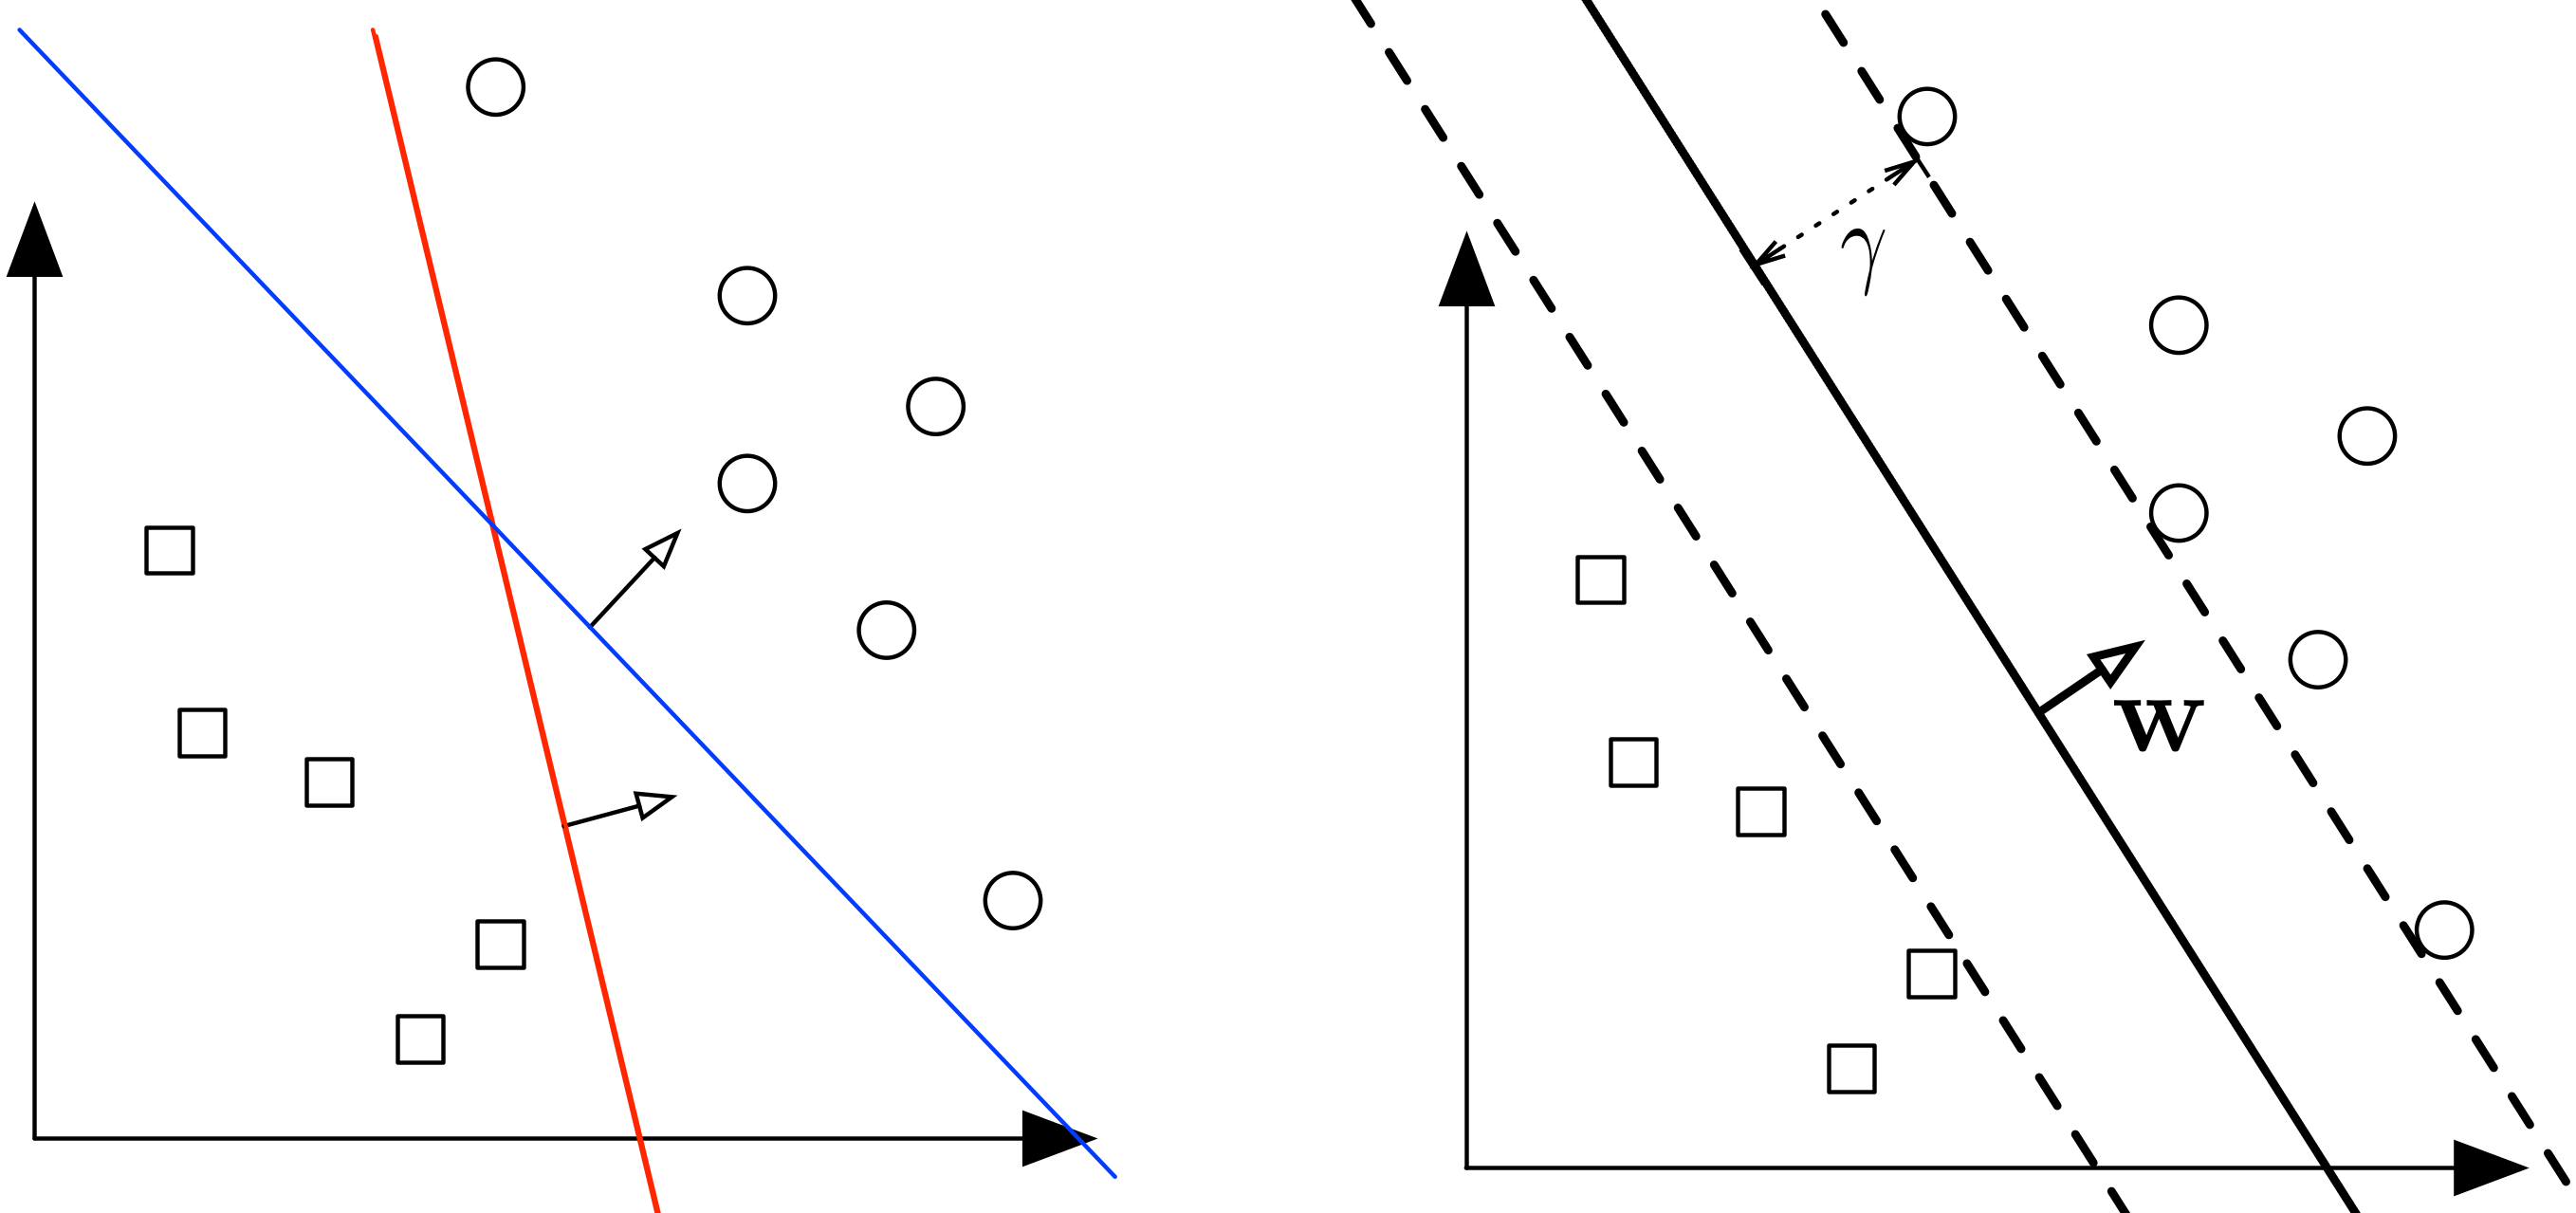
\includegraphics[scale=0.5]{img/margin.png}
    \caption{Optimálna separačná nadrovina \cite{Lecture_SVM}.}
    \label{fig:margin}
\end{figure}

V prípade, kedy dáta nie sú lineárne separovateľné, využívajú \textbf{jadrový trik}, ktorý pomocou \textbf{jadrovej funkcie} dáta transformuje do priestoru vyššej dimenzie, v ktorej už~lineárne separovateľné sú. SVM modely taktiež nevyžadujú úplnú lineárnu separabilitu, v~prípade, že~sa~dosiahnuť nedá, sa používa mäkký okraj\footnote{V anglickom jazyku \textit{soft margin}.}, ktorý umožňuje aj nesprávnu klasifikáciu. Tá je penalizovaná, čím prispieva k zmene predpisu nadroviny. Keďže transformácia dát do vyšších dimenzií vie byť výpočtovo náročná, jadrový trik využíva na transformáciu skalárne súčiny príznakov. Jadrové funkcie používajú rôzne jadrá, dve často využívané sú \textbf{polynomiálne jadro} \ref{eq:6}, kde~pre~\textit{d}=1 dostávame \textbf{lineárne jadro}, a \textbf{Gaussovské (RBF) jadro} \ref{eq:7}, kde \textit{\( \gamma \)} reguluje šírku Gaussovskej krivky. Menšia hodnota znamená hladšiu rozhodovaciu hranicu, väčšia hodnota naopak členitejšiu \cite{Cristianini_Scholkopf_2002}\cite{Suthaharan2016}.

\vspace{5pt}
\noindent
\begin{minipage}[t]{.45\textwidth}
    \begin{equation} 
        \label{eq:6}
        K(x_i,x_j) = (x_i^{T} x_j)^{d}
    \end{equation}
\end{minipage}
\hfill
\begin{minipage}[t]{.45\textwidth}
    \begin{equation} 
        \label{eq:7}
        K(x_i,x_j) = {e^{-\gamma ||x_i - x_j||^{2}}}
    \end{equation}
\end{minipage}
\vspace{5pt}

Castaño a spol. \cite{Castao2017} vo svojej publikácii skúmajú klasifikáciu pomocou SVM do dvoch tried - normálne EKG a znečistené pohybovým artefaktom. Použité dáta boli získané v riadenom experimente podobne ako naše, skúmaná bola iba jedna pohybová aktivita a to pohyb hornými končatinami. Namerané dáta boli rozdelené na segmenty o dĺžke 1.2 sekundy, korešpondujúce s~jedným úderom srdca. Skúmali SVM s lineárnym aj polynomiálnym jadrom, najlepšie výsledky dosiahli pomocou Gaussovského jadra. Kher a spol. \cite{Kher2015} riešia problém klasifikácie rôznych pohybových aktivít - pohyby hornými končatinami, rotácie v páse a chôdza. Ich prístup je odlišný v tom, že na klasifikáciu pomocou SVM nepoužívajú nespracovaný EKG signál, ale z neho extrahované príznaky pomocou rôznych transformácií, napríklad vlnkovej transformácie. Pomocou Gaussovského jadra dosiali presnosť 95 \%, kvôli využitiu transformácií táto metóda nie je vhodná na klasifikáciu v reálnom čase.


%---------------------------------------------------------------
\section{Vyhodnotenie klasifikácie do viacerých tried}
%---------------------------------------------------------------

%---------------------------------------------------------------
\subsection{Matica zámen}
%---------------------------------------------------------------

Ako hlavnú metriku na vyhodnotenie úspešnosti klasifikácie sme zvolili maticu zámen, ktorá reprezentuje klasifikáciu do viacerých tried ako kontingenčnú tabuľku, kde riadky predstavujú skutočnú hodnotu a stĺpce predikovanú hodnotu. Na diagonále sa nachádzajú správne predikcie, zatiaľ čo na ostatných pozíciach nesprávne. Hodnoty v jednotlivých poliach matice môžeme uvádzať v absolútnom, alebo normalizovanom tvare, teda v percentuálnom podeli \cite{grandini2020metrics}. V našom prípade budeme kvôli nevyváženosti dátovej sady výsledky klasifikácie uvádzať spravidla v normalizovanom tvare.

\begin{figure}[H]
    \centering    
    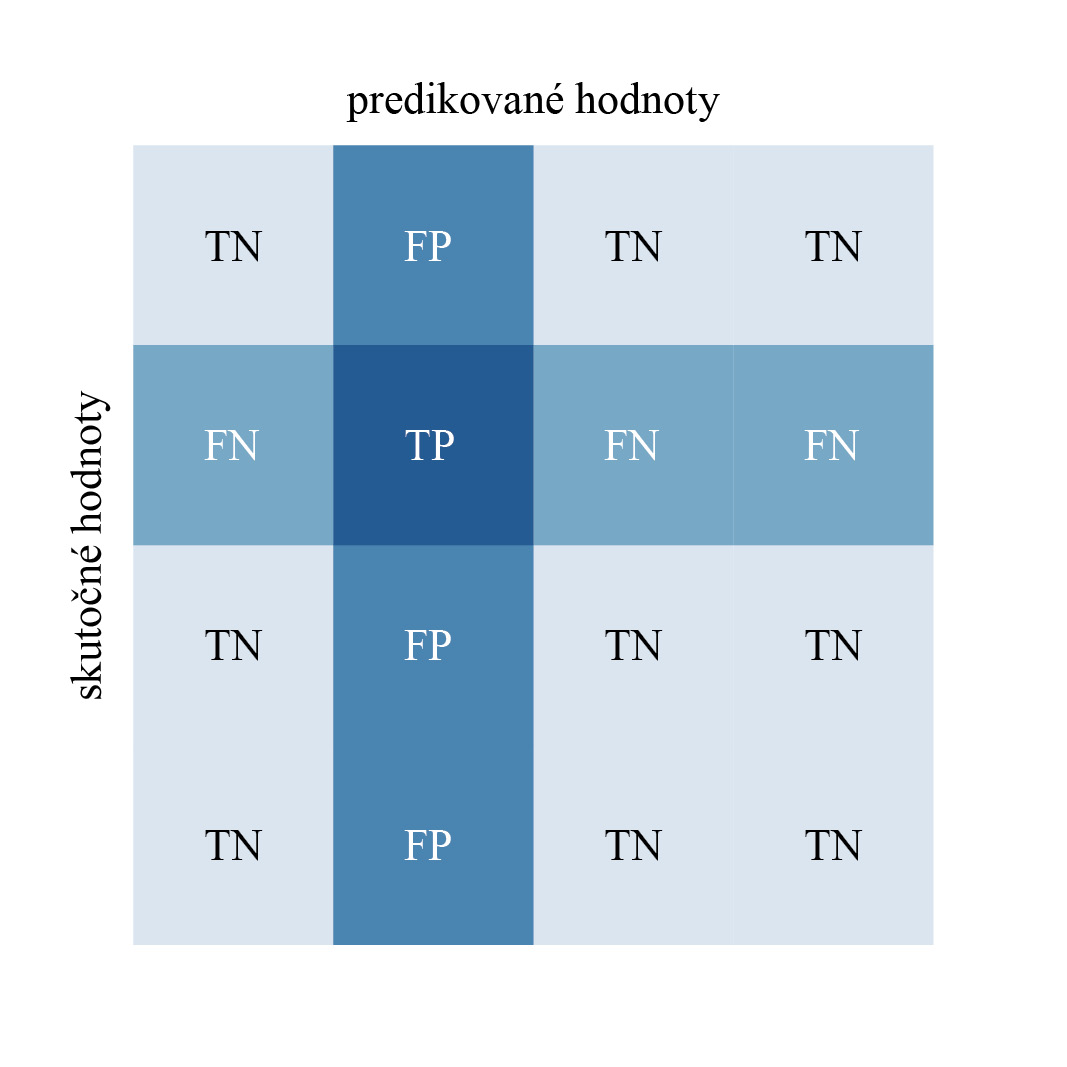
\includegraphics[scale=0.22]{img/confusion_martix.jpg}
    \caption{Matica zámen pre klasifikáciu do viacerých tried.}
    \label{fig:confusion_matrix}
\end{figure}

\noindent Maticu zámen interpretujeme v kontexte klasifikácie do viacerých tried z pohľadu jednej triedy \textit{x} tak, ako je uvedené na obrázku \ref{fig:confusion_matrix}.

\begin{itemize}
    \item \textbf{TP (True positive)} - počet segmentov triedy \textit{x}, ktoré boli správne klasifikované.
    \item \textbf{FN (False negative)} - počet segmentov triedy \textit{x}, ktoré boli nesprávne klasifikované.
    \item \textbf{TN (True negative)} - počet segmentov triedy inej ako \textit{x}, ktoré boli správne klasifikované.
    \item \textbf{FP (False positive)} - počet segmentov triedy inej ako \textit{x}, ktoré boli nesprávne klasifikované.
\end{itemize}

V texte budeme tieto metriky ďalej uvádzať iba pomocou vyššie uvedených skratiek. Na základe hodnôt uložených v matici zámen vieme počítať ďalšie metriky, vybrané z nich zadefinujeme nižšie.

%---------------------------------------------------------------
\subsection{Accuracy}
%---------------------------------------------------------------

Presnosť, v anglickom znení \textit{accuracy}, je definovaná ako podiel segmentov, ktoré model určil správne, voči celkovému počtu segmentov a dá sa vyjadriť vzťahom \ref{eq:8} \cite{grandini2020metrics}.

\begin{equation} 
    \label{eq:8}
    ACC = \frac{TP + TN}{TP + TN + FP + FN}
\end{equation}

%---------------------------------------------------------------
\subsection{Recall}
%---------------------------------------------------------------

\textit{Recall}, alebo senzitivita, prípadne \textit{true positive rate (TPR)}, je definovaný ako podiel segmentov vybranej triedy, ktoré model určil správne \cite{grandini2020metrics}. Dá sa vyjadriť vzťahom \ref{eq:9} a v normalizovanom tvare matice zámen leží senzitivita pre jednotlivé triedy na diagonále.

\begin{equation} 
    \label{eq:9}
    Recall = \frac{TP}{TP + FN}
\end{equation}

%---------------------------------------------------------------
\subsection{Precision}
%---------------------------------------------------------------

\textit{Precision}, alebo \textit{positive predictive value (PPV)}, je definovaná ako podiel segmentov označených ako patriacich do vybranej triedy, ktoré skutočne do tejto triedy patria a dá sa vyjadriť vzťahom \ref{eq:10} \cite{grandini2020metrics}.

\begin{equation} 
    \label{eq:10}
    Precision = \frac{TP}{TP + FP}
\end{equation}

%---------------------------------------------------------------
\subsection{F1 Score}
%---------------------------------------------------------------

\textit{F1 Score} je metrika, ktorá počíta harmonický priemer \textit{precision} a \textit{recall} a je vhodná na vyhodnocovanie predikcií na nevyvážených dátach. Pre každú triedu zvlášť sa dá vyjadriť vzťahom \ref{eq:11} a následne sa v prípade klasifikácie do viacerých tried počíta vážený priemer získaných hodnôt podľa vzťahu \ref{eq:12} \cite{grandini2020metrics}.

\begin{equation} 
    \label{eq:11}
    F1 \ Score = \frac{2 \times Precision \times Recall}{Precision + Recall}
\end{equation}

\begin{equation} 
    \label{eq:12}
    Weighted \ F1 \ Score = \sum_{i=1}^{N} w_i \times F1 \ Score_i
\end{equation}



%---------------------------------------------------------------
\chapter{Metodika experimentu}
%---------------------------------------------------------------

V tejto kapitole podrobne popíšeme priebeh riadeného experimentu uskutočneného so zámerom získania dát pre účely tejto práce. Taktiež popíšeme všetky potrebné zariadenia využité pri~jednotlivých meraniach, ale aj vytvorené nástroje na vizualizáciu a kontrolu získaných EKG zázna-mov a ich následnú anotáciu. Cieľom experimentu bolo vyhotoviť dátovú sadu, vhodnú na~použi-tie pri trénovaní a testovaní modelov umelej inteligencie, ktorých úlohou je detegovať pohybové artefakty s čo najväčšou presnosťou.


%---------------------------------------------------------------
\section{Popis subjektov}
%---------------------------------------------------------------

Keďže v tejto práci neanalyzujeme EKG zo zdravotného hľadiska, v dátach nepredpokladáme veľkú interpersonálnu variabilitu čo sa týka výskytu pohybových artefaktov. Preto boli subjekty vyberané náhodne a neboli stanovené žiadne podmienky na účasť, okrem zdravotnej spôsobilosti vykonávať jednotlivé úkony v experimente. Jediné obmedzenie, a to aby boli subjekty v produktívnom veku, priamo vyplýva zo zamerania práce a využitia pre zásahové zložky. Interpersonálna variabilita z hľadiska priebehu EKG signálu je naopak žiadúca, keďže detekcia by mala byť voči tejto variabilite odolná. Experimenty sme preto vykonávali na viacerých subjektoch.

Experimentu sa zúčastnilo 10 dobrovoľníkov, pričom 3 z nich boli ženského pohlavia a~7~mužského. Vekové rozmedzie subjektov bolo 21 - 42 rokov. Priemerná váha bola 67,67\( \pm \)9,53 kg pre ženy a 81,29\( \pm \)7,99 kg pre mužov, priemerná výška 171,33\( \pm \)6,34 cm pre ženy a 181,71\( \pm \)5,67 cm pre mužov. Tieto hodnoty sú primerané jednotlivým pohlaviam, nenachádzajú sa v nich žiadne extrémy, rovnako aj fyzická kondícia jednotlivých subjektov bola primeraná ich veku. Priemerná hodnota obvodu hrudníka bola 80\( \pm \)6,53 cm pre ženy a 93\( \pm \)6,61 pre mužov. Táto hodnota je~u~mužov výrazne vyššia ako u žien, čo je dôležitá informácia kvôli porovnaniu s najmenším možným nastavením obvodu hrudných pásov. Keďže pri monitorovaní pomocou plošných suchých a textilných elektród je kľúčové zabezpečenie dostatočného kontaktu elektród s kožou, nastavenie pásu môže byť limitujúce pre osoby s úzkym hrudníkom.

\begin{table}[H]\centering
\caption[Prehľad subjektov experimentu.]{~Prehľad subjektov experimentu.}\label{tab:subjects}
    \begin{tabular}{c|c|c|c|c|c}
    	\textbf{ID} & \textbf{Pohlavie} & \textbf{Vek} & \textbf{Výška (cm)} & \textbf{Váha (kg)} & \textbf{Obvod hrudníka (cm)} \tabularnewline \hline 
     	01        	          &  M                & 36           & 182                 & 94                 & 105                          \tabularnewline \hline
        02        	          &  M                & 22           & 193                 & 80                 & 97                           \tabularnewline \hline
        03        	          &  Ž                & 42           & 165                 & 55                 & 72                           \tabularnewline \hline
        04        	          &  M                & 23           & 184                 & 88                 & 87                           \tabularnewline \hline
        05        	          &  Ž                & 25           & 180                 & 78                 & 88                           \tabularnewline \hline
        06        	          &  Ž                & 24           & 169                 & 70                 & 80                           \tabularnewline \hline
        07        	          &  M                & 38           & 180                 & 75                 & 91                           \tabularnewline \hline
        08        	          &  M                & 30           & 182                 & 70                 & 84                           \tabularnewline \hline
        09        	          &  M                & 21           & 173                 & 75                 & 90                           \tabularnewline \hline
        10        	          &  M                & 21           & 178                 & 87                 & 97                           \tabularnewline
    \end{tabular}
\end{table}


%---------------------------------------------------------------
\section{Použitý hardware}
%---------------------------------------------------------------

Na snímanie EKG bol použitý špecializovaný analógový front-end \textbf{AD8232}~\cite{Analog_Devices} od firmy Analog Devices, určený na precízne meranie biopotenciálov v prenosných a fitnes EKG. Na realizáciu meracieho modulu bolo zvolené priepustné pásmo pre EKG signál v rozsahu 0,05 až 150 Hz a celkové zosilenie 500. Vďaka tomu sú prenášané všetky významné frekvencie v EKG signáli a kvalita signálu sa pri kľudovom snímaní blíži klinickému EKG. Okrem základnej analógovej pásmovej priepusti s uvedeným priepustným pásmom nie je so signálom zámerne vykonávaná žiadna ďalšia analógová a následne ani číslicová filtrácia, zariadenie teda poskytuje hrubé dáta. Použité obvodové riešenie ďalej obsahuje zapojenie pre aktívnu referenčnú elektródu, ktoré pri~trojelektródovom pripojení pacienta použitom v tejto práci zaistí zvýšenie činiteľa potlačenia súfázového signálu (CMRR). Izolačné napätie obvodu je 7000 V, maximálny merací rozkmit amplitúdy vstupného EKG signálu je špička-špička 6 mV. Modul tiež disponuje digitálnymi signálovými vodičmi na indikáciu stavu pripojenia elektród. Digitalizácia výstupného analógové-ho signálu je realizovaná 32 bitovým mikrokontrolérom rodiny AT SAMD 21 (architektúra Arm Cortex-M0), vybaveným firmware, ktorý zaisťuje digitalizáciu EKG signálu z analógového front-endu pomocou vstavaného 12 bitového analógovo-digitálneho (AD) prevodníku, serializáciu signálu a následný prenos cez vstavané USB rozhranie do pripojeného PC. Ekvidistantné vzorkovanie EKG signálu je nastavené na frekvenciu 500 Hz, čím zodpovedá klinickým štandardom pre~snímanie EKG signálu. Zariadenie je súčasťou experimentálneho systému na sledovanie vitálnych funkcií členov integrovaného záchranného systému (IZS), najmä hasičov, vyvíjaného na Katedre informačných a komunikačných technológií v lekárstve FBMI ČVUT.  

\begin{figure}[H]
    \centering
    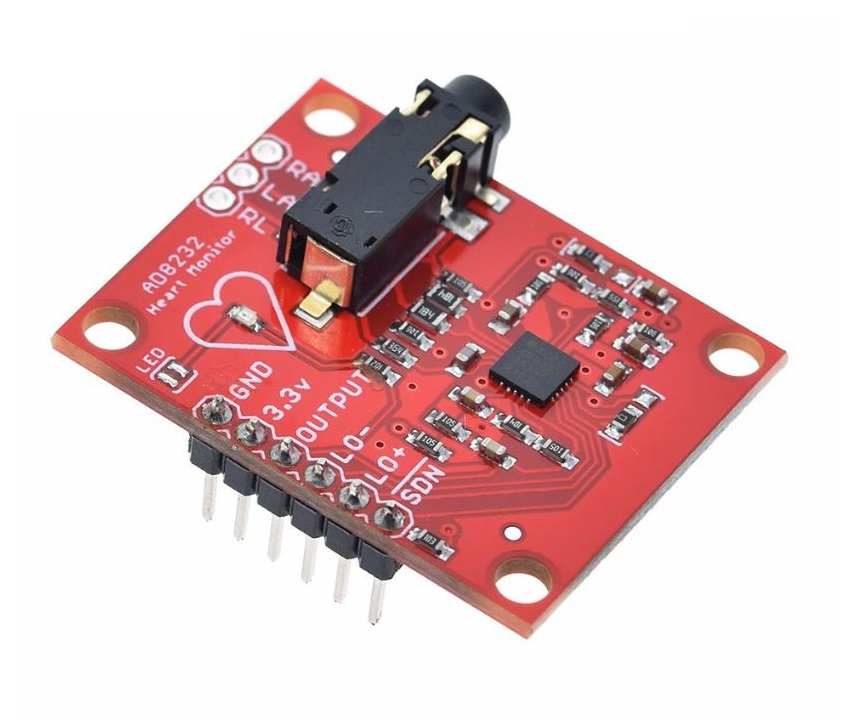
\includegraphics[scale=0.24]{img/AD8232.jpg}
    \caption{Vývojový modul s obvodom AD8232 \cite{Sharvielectronics_2022}.}
    \label{fig:HW}
\end{figure}


%---------------------------------------------------------------
\section{Použitý software}
%---------------------------------------------------------------

%---------------------------------------------------------------
\subsection{Vizualizácia a záznam EKG}
%---------------------------------------------------------------

Software ju súčasťou vyššie popísaného hardwarového riešenia zariadenia na snímanie, digitalizáciu a prenos EKG. Umožňuje automatickú detekciu pripojeného EKG modulu, vyčítanie a~vizualizáciu EKG dát v reálnom čase a ukladanie do súboru. Software umožňuje konfiguráciu počtov kanálov, ich rozsahov, úpravu komunikačného protokolu, robustnú detekciu R-vĺn v EKG signáli pomocou Hamilton-Tompkinsovho algoritmu a signalizáciu srdečného rytmu akustickým signálom. Software je implementovaný v programovacom jazyku Rust\footnote{https://www.rust-lang.org} a je súčasťou experimentálneho systému na snímanie biopotenciálov v teréne, uvedeného v predošlej kapitole. Software je multiplatformný a umožňuje beh pod operačnými systémami MS Widnows, MacOS a~Linux.

\begin{figure}[H]
    \centering
    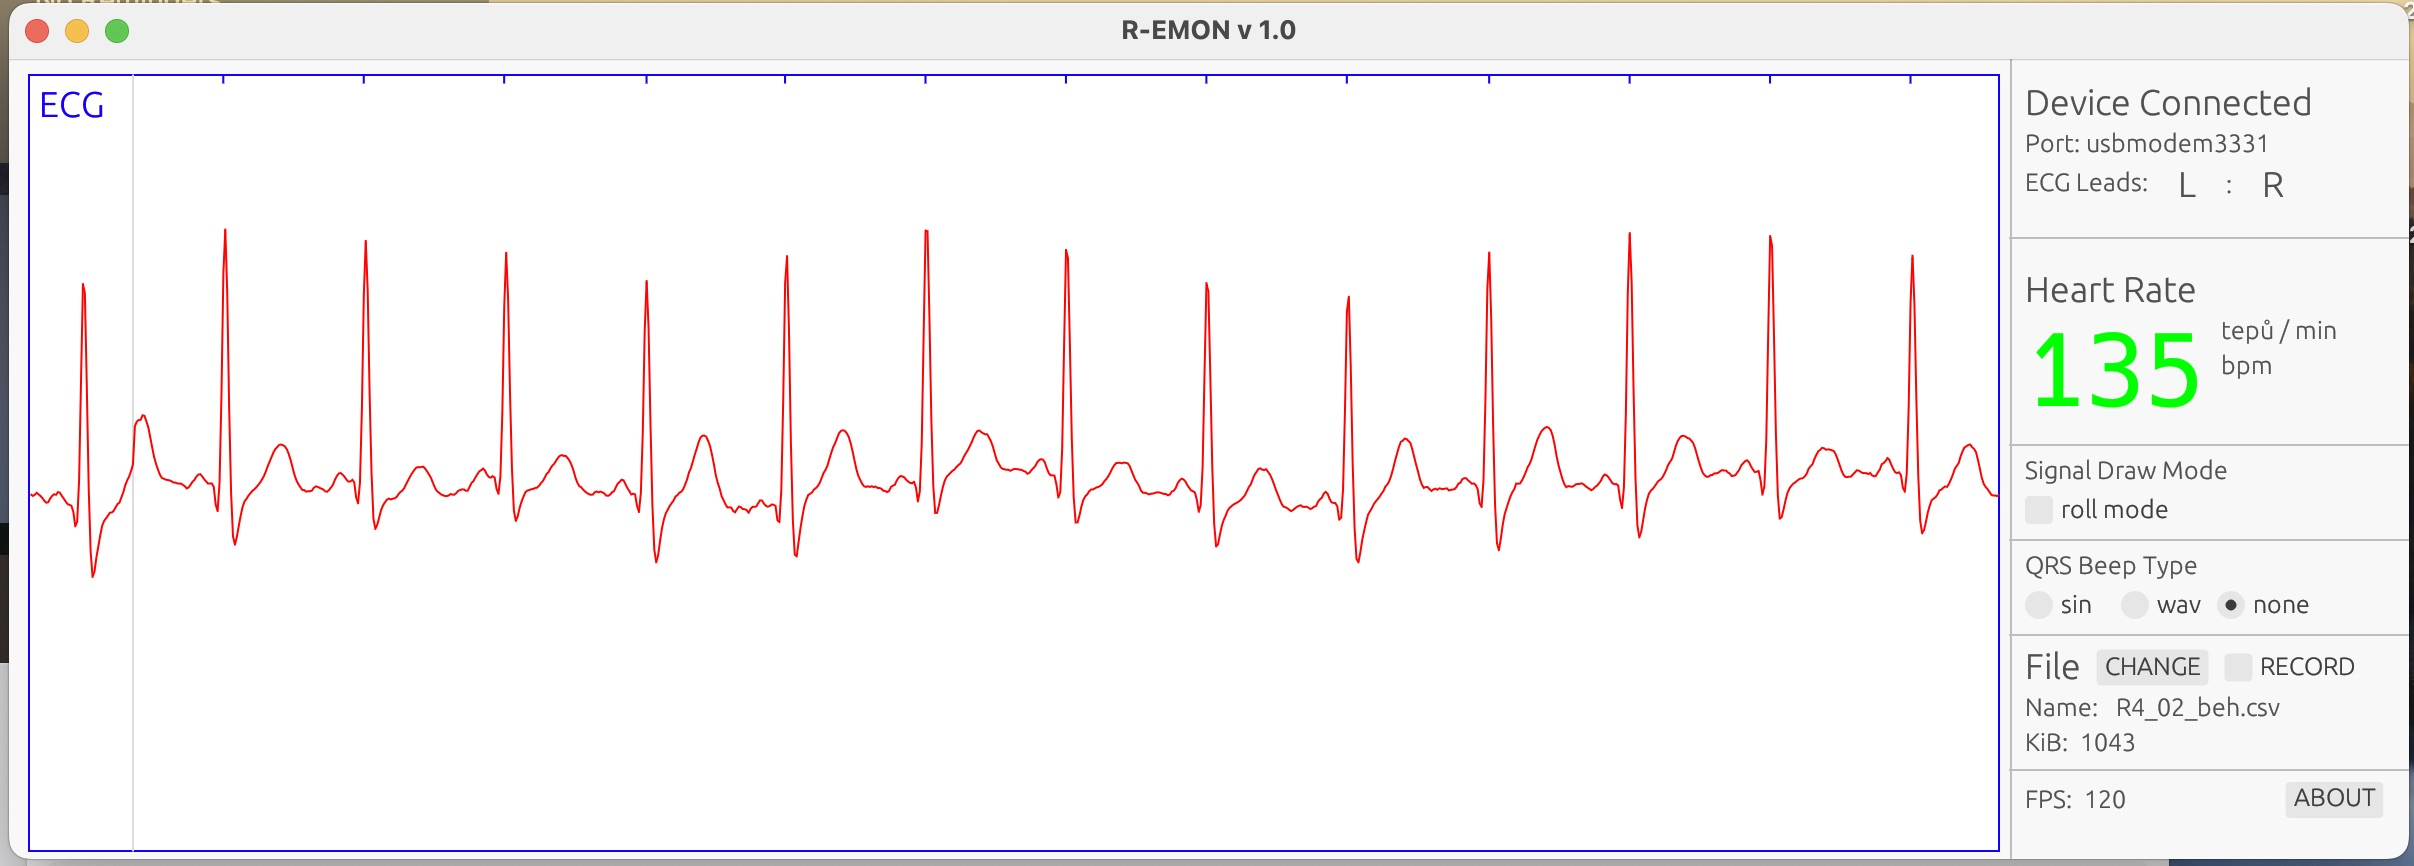
\includegraphics[scale=0.172]{img/recording_sw.jpeg}
    \caption{Software na vizualizáciu a záznam EKG.}
    \label{fig:SW_recording}
\end{figure}

%---------------------------------------------------------------
\subsection{Manuálna anotácia dát}
%---------------------------------------------------------------

Kvôli nutnosti manuálne anotovať namerané EKG dáta bolo vytvorené jednoduché grafické rozhranie. Okrem samotnej anotácie dát toto rozhranie slúži aj na zobrazenie a kontrolu nameraných dát z jednotlivých experimentov. Zdrojový kód je napísaný v programovacom jazyku \textbf{Python~3.8}\footnote{https://www.python.org}, s inými verziami nemusí byť plne kompatibilný. Užívateľské rozhranie bolo vytvorené pomocou \textbf{PyQt5}\footnote{https://pypi.org/project/PyQt5/5.8/}, ktoré poskytuje programátorské rozhranie medzi knižnicou na tvorbu grafických aplikácií Qt a jazykom Python. EKG krivka je zobrazená na grafe vykreslenom pomocou knižnice \textbf{Matplotlib}\footnote{https://matplotlib.org}. Kompletný zoznam knižníc potrebných na spustenie aplikácie je~možné nájsť v zložke so zdrojovými kódmi v súbore \textit{requirements.txt}.

\begin{figure}[H]
    \centering
    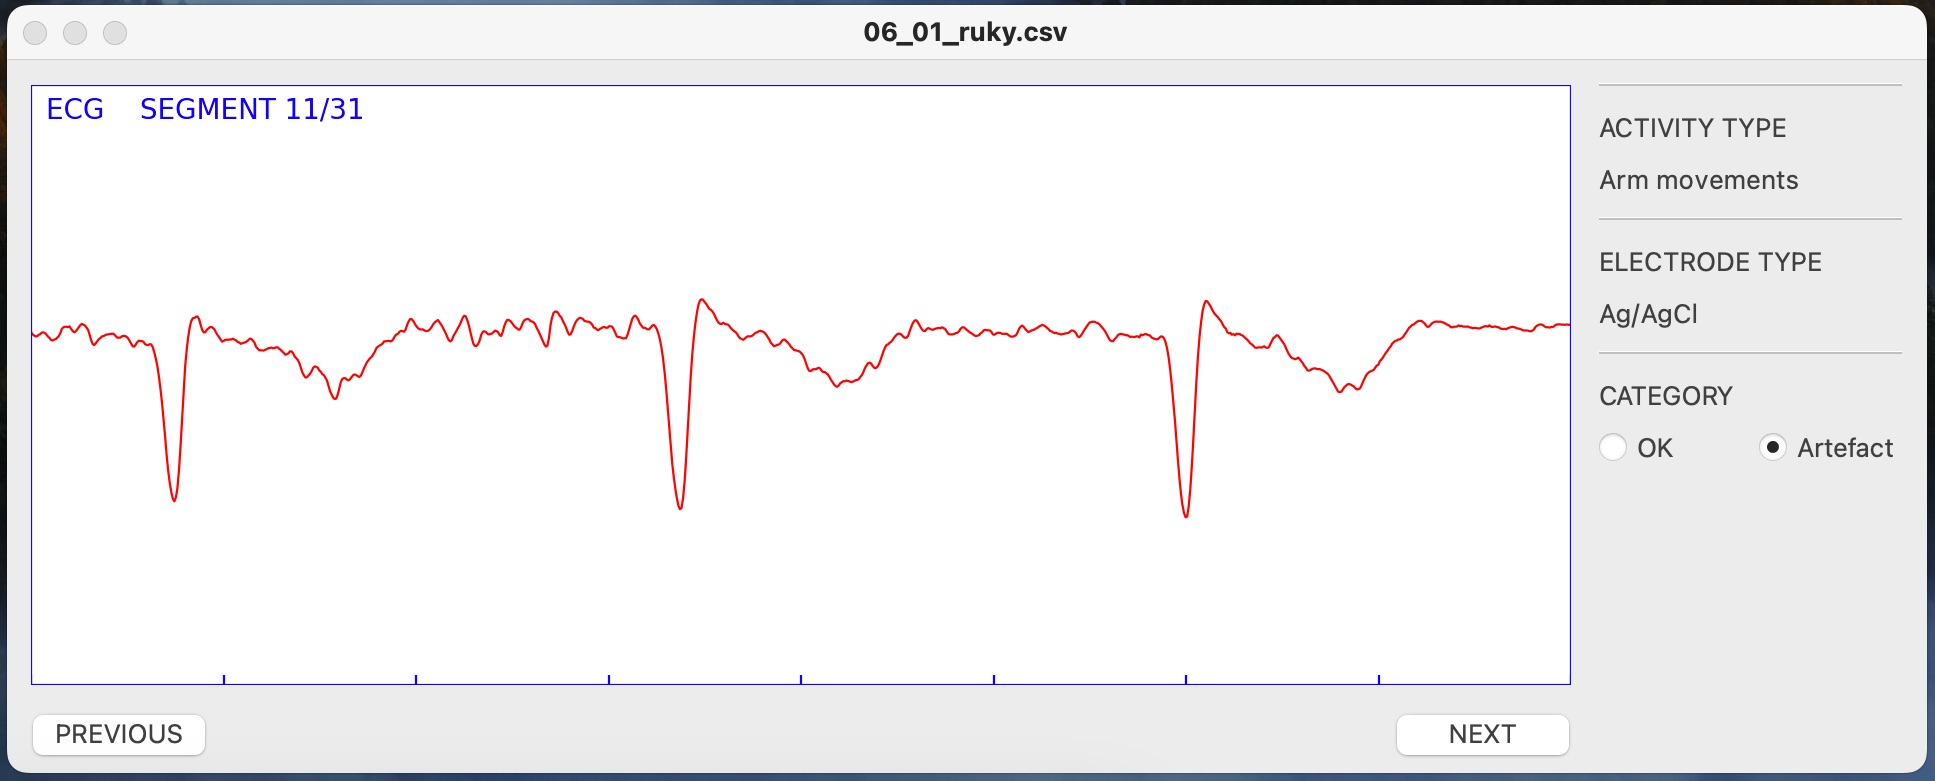
\includegraphics[scale=0.215]{img/annotation_sw.jpeg}
    \caption{Grafické rozhranie na manuálnu anotáciu EKG dát.}
    \label{fig:SW_labels}
\end{figure}

Grafické rozhranie umožňuje navigáciu cez jednotlivé segmenty EKG signálu, pričom ich~dĺžka je voliteľná. Na pohyb medzi segmentmi sa dajú použiť buď tlačidlá umiestnené pod~oknom, v ktorom sa zobrazuje aktuálny segment, alebo ľavá a pravá šípka na klávesnici. V ľavom hornom rohu okna zobrazujúceho aktuálny segment sa nachádza číslo aktuálneho segmentu a~ich~celkový počet. V paneli na pravej strane okna sa nachádza typ pohybovej aktivity a~použitých elektród, oboje sú odvodené od názvu súboru. V neposlednom rade sa~tu~nachádzajú aj prepínacie tlačidlá, ktorými sa anotuje daný segment podľa rozličnej úrovne znečistenia pohybovým artefaktom. Tieto tlačidlá sa dajú opäť ovládať priamo kliknutím, alebo sa dá na~ich~pre-pínanie využiť medzerník na klávesnici. Pri otvorení vstupného súboru, ktorý chce používateľ anotovať, sa automaticky vytvorí výstupný \textit{.csv} súbor, rovnako sa pri zmene stavu prepínacieho tlačidla označujúceho artefakt tento súbor automaticky prepíše, explicitné ukladanie nie je nutné. 

Používateľské rozhranie je možné spustiť pomocou príkazu \textbf{python3 data\_labeler.py} z príslušnej zložky, a voliteľné parametre sú nasledovné:

 \noindent \textbf{data\_labeler.py [-l segment\_length] [-f sampling\_rate] [-s starting\_segment] input\_file}
 
\begin{tabbing}
    \indent \textbf{input\_file (str)} \quad\quad\quad\quad \= - názov vstupného súboru, musí byť súbor typu \textit{.csv}\\
                                                            \> nachádzajúci sa v zložke \textit{/data}\\
    \indent \textbf{segment\_length (int)}                  \> - dĺžka segmentu v sekundách, predvolená na 5 sekúnd\\
    \indent \textbf{sampling\_rate (int)}                   \> - vzorkovacia frekvencia vstupného súboru, predvolená na\\
                                                            \> 500 vzoriek za sekundu\\
    \indent \textbf{starting\_segment (int)}                \> - číslo počiatočného segmentu na zobrazenie, predvolené na\\
                                                            \> prvý segment\\
\end{tabbing}

\newpage

%---------------------------------------------------------------
\section{Použité elektródy}
%---------------------------------------------------------------

 Séria úkonov bola vykonávaná najskôr s gélovými elektródami, následne s hrudným pásom s~plošnými elektródami z nerezovej ocele (Obr. \ref{fig:electrodes} dole) a na záver s hrudným pásom s textilnými elektródami (Obr. \ref{fig:electrodes} hore). Rozmery jednej elektródy z nerezovej ocele sú 6 x 4,5 cm a rozmery jednej textilnej elektródy 6 x 4 cm. Jednorazové Ag/AgCl elektródy boli použité konkrétne EKG H34 SG Kendall\textsuperscript{TM} od firmy Covidien\textsuperscript{TM}, obsahujúce hydrogél vhodný na dlhodobé monitorovanie. Oba hrudné pásy sú súčasťou vyššie uvedeného experimentálneho systému vyvíjaného na FBMI ČVUT.

 \begin{figure}[H]
    \centering
    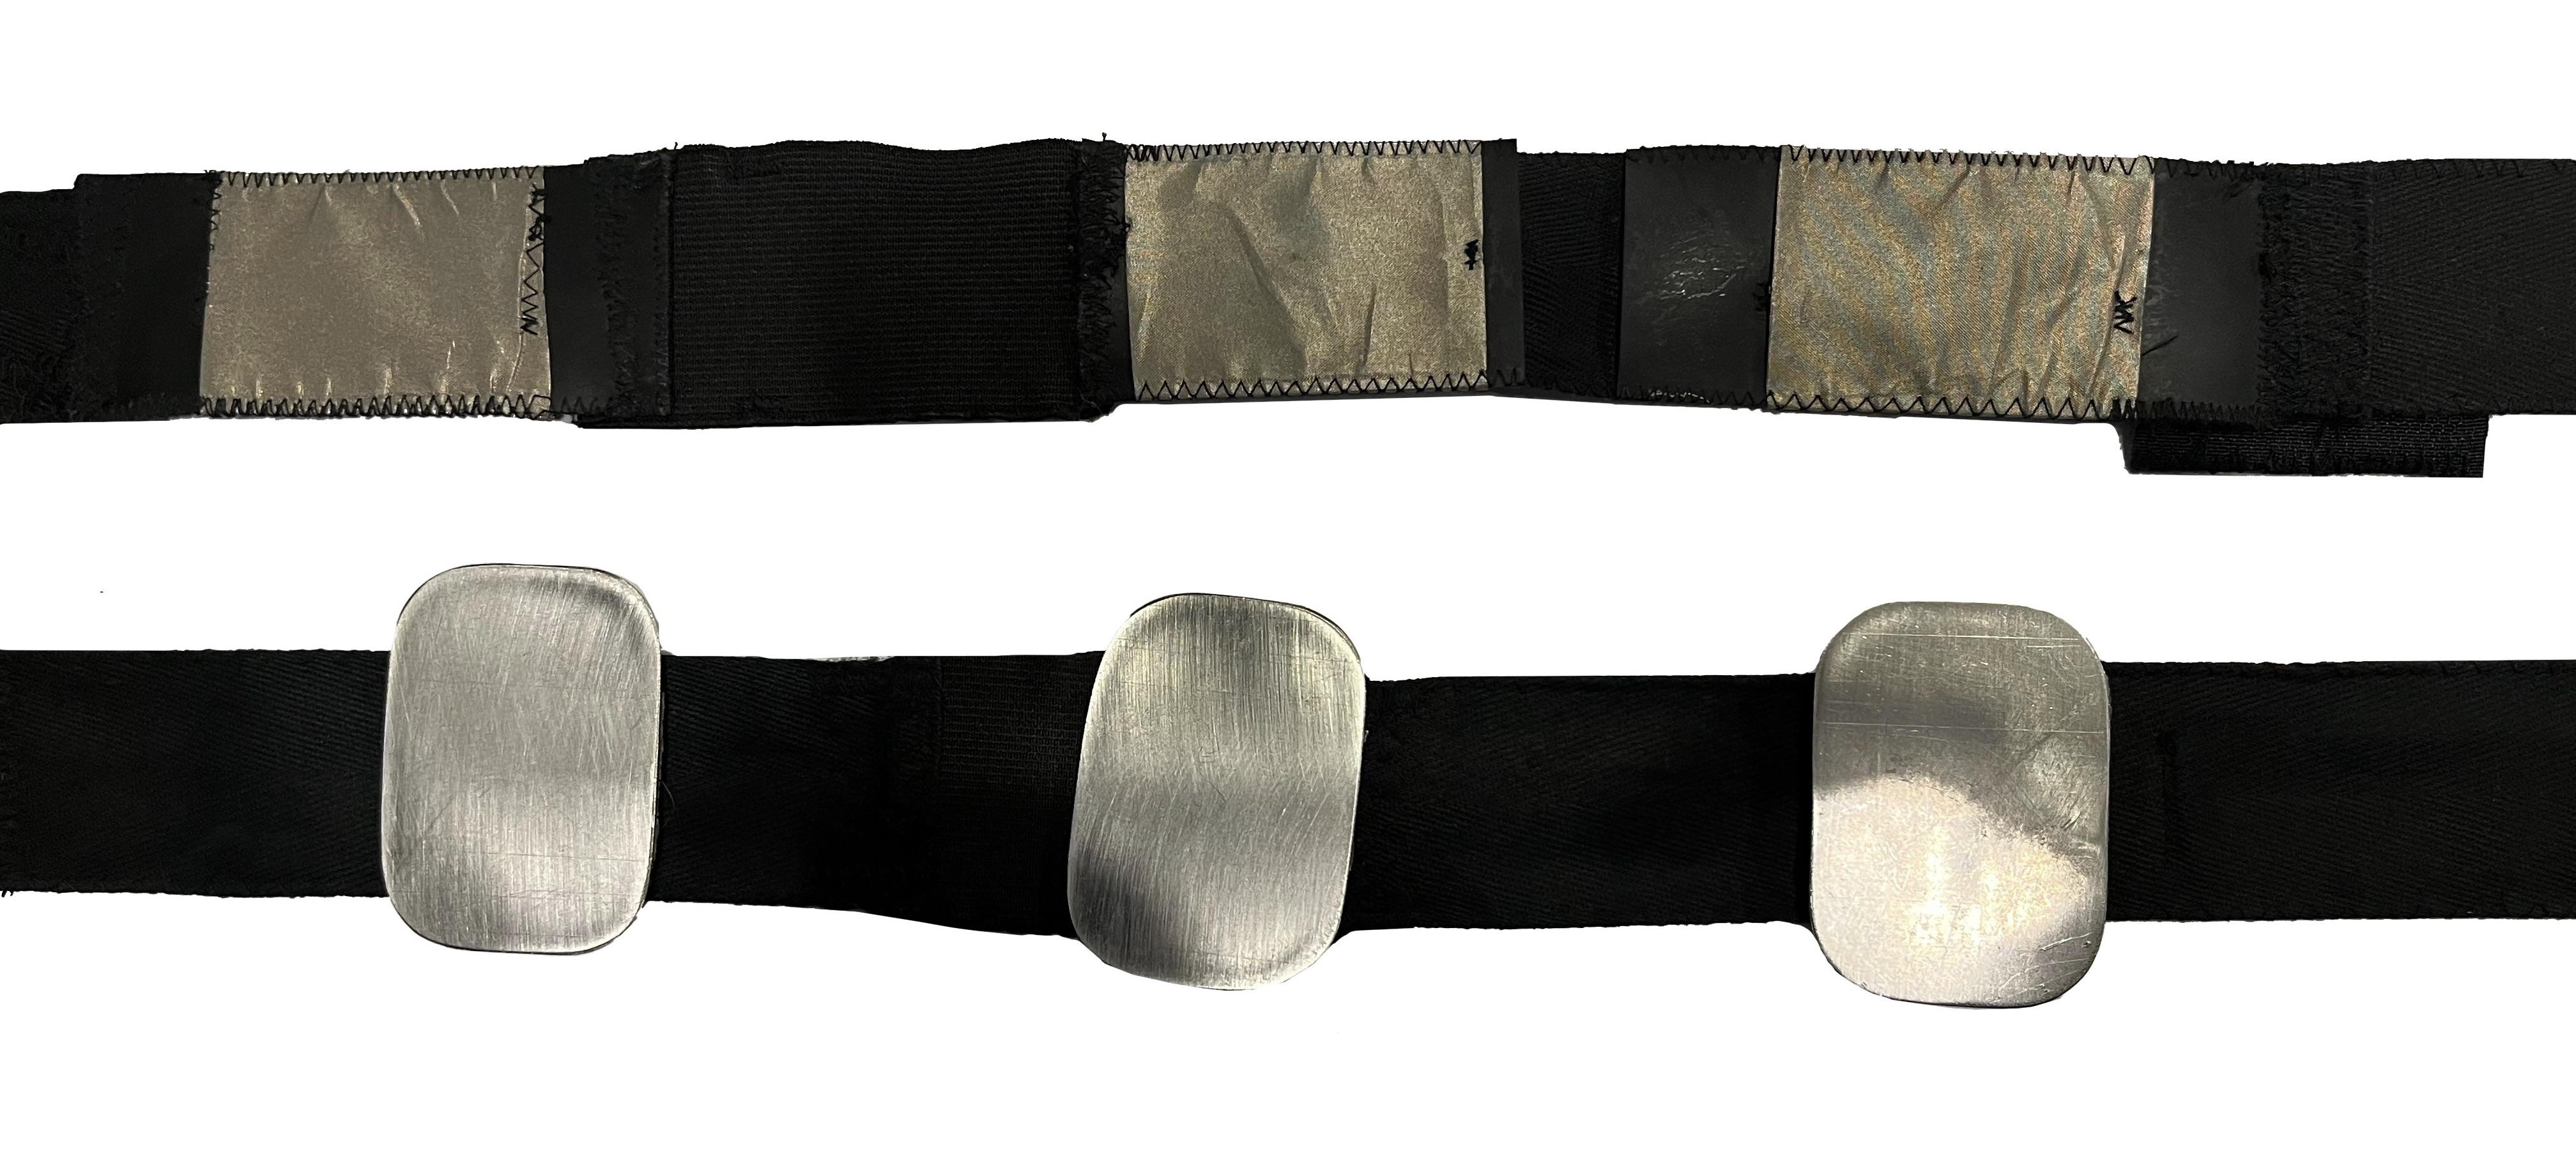
\includegraphics[scale=0.1]{img/electrodes.jpg}
    \caption{Hrudný pás s elektródami z nerezovej ocele a textilnými elektródami.}
    \label{fig:electrodes}
\end{figure}
 
 Poradie elektród bolo zvolené tak, aby sme minimalizovali nutnosť prípravy pokožky subjektov. Keďže gélové elektródy obsahujú vodivú zložku, nie je potrebná žiadna ďalšia príprava pokožky. Elektródy z nerezovej ocele a textilné elektródy fungujú lepšie ak je subjekt trochu zahriaty a tým pádom spotený, keďže pot zvyšuje vodivé vlastnosti medzi kožou a elektródou. Nadmerné potenie môže viesť k vytvoreniu takzvaného potného mostíka, kedy dochádza k skratu elektród, prípadne výrazne zníženému odporu, následkom čoho je meraný EKG signál utlmený na takmer nemerateľný. Zvolené úkony však nepredstavovali takú záťaž, aby zapríčinili nadmerné potenie subjektov. V prípade, že subjekt nebol po prvej sérii úkonov dostatočne spotený, simulovali sme tento jav miernym zvlhčením pokožky v miestach dotyku elektród.

 Keďže ide o terénne monitorovanie, umiestnenie elektród nebolo presne stanovené, ako~pri~štandardizovanom snímaní EKG signálu. Oba hrudné pásy boli umiestnené v oblasti pod~prsným svalom a polohy gélových elektród kopírovali pozíciu suchých elektród na páse. Jedna elektróda bola umiestnená zhruba v strede hrudníka, ostatné dve symetricky na ľavej a~pravej strane rebier. Dôležité pre kvalitu signálu bolo, aby sa elektródy nenachádzali pod úrovňou rebier. Ako nulová elektróda bola zvolená prostredná, ostatné dve boli aktívne. Napojením na~nositeľný snímač bol takto vytvorený 1-zvodový systém na záznam EKG.

\newpage

%---------------------------------------------------------------
\section{Priebeh experimentu}
%---------------------------------------------------------------

Po príchode na pracovisko bol každý subjekt oboznámený s priebehom a dĺžkou experimentu, a bol požiadaný o podpísanie informovaného súhlasu (Dodatok \ref{chap:suhlas}). Subjekt bol informovaný o~tom, že účasť na experimente je dobrovoľná, aj o možnosti kedykoľvek svoju účasť na experimente ukončiť, a to bez udania dôvodu. Taktiež bol informovaný o možnosti odmietnuť vykonávať akýkoľvek úkon v prípade, že by bol pre neho príliš fyzicky náročný. Následne bol každý subjekt požiadaný o vyplnenie dotazníku (Dodatok \ref{chap:dotaznik}), v ktorom sa zisťovali nasledovné údaje: meno, pohlavie, vek, výška, váha a obvod hrudníka. Dotazník obsahuje aj otvorenú časť týkajúcu sa pohybových obmedzení a ochorení kardiovaskulárneho a respiračného systému, ktoré by znemožňovali účasť v experimente. V kontexte dotazníka bol každý poučený, že záznamy, podľa ktorých je možné subjekt identifikovať, budú uschované ako dôverné dokumenty a nebudú verejne sprístupnené. Taktiež že v prípade, kedy budú výsledky štúdie publikované, jeho totožnosť nebude zverejnená. V informovanom súhlase bolo zdôraznené aj to, že zo získaných dát nebudú vyvodzované žiadne závery týkajúce sa zdravotného stavu.

Podpisom informovaného súhlasu a vyplnením dotazníku subjekt potvrdil, že sa ho netýkajú žiadne z nasledovných vylučovacích kritérií. Fáza experimentu, ktorá zahŕňa fyzickú záťaž, vyžadovala vylúčenie osôb, ktoré trpia závažným ochorením respiračného alebo kardiovaskulárneho systému. Kvôli pohybu na bežiacom páse bolo potrebné z experimentu vylúčiť aj osoby trpiace zníženou pohyblivosťou, alebo zníženou funkciou rovnovážneho systému, a to aj v prípade zapríčinenia konzumáciou alkoholu, alebo inej omamnej látky. Dĺžka experimentu na jeden subjekt bola stanovená na 30 minút - 15 minút rezervovaných na samotné merania a~zvyšných 15~minút na réžiu spojenú s výmenou elektród a prechodom medzi jednotlivými pohybovými aktivitami. Je dôležité spomenúť, že dĺžka vykonávaného úkonu nebola vždy presne jedna minúta, ide o približný časový údaj. Napríklad pri postupnej zmene rýchlosti pohybu na~bežiacom páse bolo potrebné počkať na ustálenie rýchlosti.

Poradie jednotlivých úkonov v rámci experimentu bolo stanovené tak, ako je uvedené v~tabuľke \ref{tab:activities}. Takto stanovená séria úkonov bola vykonávaná tri krát, zakaždým s iným druhom elektród. Poradie úkonov bolo pre správnosť postupu zostavené tak, aby záťaž narastala, aj~keď zvyšujúca sa srdcová frekvencia by nemala mať vplyv na výskyt pohybových artefaktov v~zázname. Navyše mal medzi každou sériou úkonov subjekt možnosť oddýchnuť si počas výmeny elektród, ktorá trvala niekoľko minút, čo umožnilo klesnutie srdcovej frekvencie späť na takmer kľudovú pred začiatkom ďalšej série úkonov. 

\begin{table}[H]\centering
\caption[Poradie pohybových aktivít.]{~Poradie pohybových aktivít.}\label{tab:activities}
    \begin{tabular}{l|c}
    	\textbf{Pohybová aktivita}  & \textbf{Doba merania vo formáte od - do (mm:ss)}        \tabularnewline \hline 
     	Kľud                        & 0:00 - 1:00                                   \tabularnewline \hline
     	Pohyby hornými končatinami	& 1:00 - 2:00                                   \tabularnewline \hline
        Chôdza 4 km/h           	& 2:00 - 3:00                                   \tabularnewline \hline
        Beh	8 km/h                  & 3:00 - 4:00                                   \tabularnewline \hline
        Drepy	                    & 4:00 - 5:00                                   \tabularnewline 
    \end{tabular}
\end{table}



%---------------------------------------------------------------
\chapter{Dátová sada}
%---------------------------------------------------------------

V nasledujúcej kapitole opíšeme štruktúru vzniknutej dátovej sady. Dáta pre účastníkov experimentu sú členené do zložiek, pričom každý subjekt ma svoju vlastnú, ktorá obsahuje všetky zaznamenané EKG dáta a k ním príslušné anotácie segmentov. Experimentu sa zúčastnilo \textbf{10~subjektov}, pre každého je nameraných niekoľko záznamov dlhých približne jednu minútu - \textbf{5~rôznych fyzických aktivít} zaznamenaných pomocou \textbf{3~rôznych typov elektród}. Dostávame teda 15~záznamov pre každý subjekt, takže dokopy \textbf{150~minútových záznamov EKG}. Každý z~týchto záznamov bol následne rozdelený na segmenty dlhé 2 sekundy, čím na záver získavame približne \textbf{4500 anotovaných segmentov}. Vzniknutá dátová sada je verejne dostupná pod GNU GPL 3.0 licenciou na GitHub repozitári Katedry informačných a komunikačných technológií v~lekárstve FBMI ČVUT.

%---------------------------------------------------------------
\section{Anotácia dátovej sady}
%---------------------------------------------------------------

Významnou časťou práce bola anotácia vzniknutej dátovej sady. Po analýze viacerých možností sme sa rozhodli dáta anotovať do štyroch rôznych kategórií, pričom každá je definovaná charakteristickými vlastnosťami. Testovali sme aj možnosť kedy sme kategórie definovali podľa viditeľnosti jednotlivých vĺn, tento postup sa však kvôli interpersonálnej variabilite priebehu EKG signálu ukázal ako problematický, keďže nie každý subjekt mal v kľudovom zázname viditeľnú P-vlnu, rovnako amplitúda T-vlny sa výrazne líšila.

Dĺžka segmentu bola na základe vyššie uvedených publikácií zvolená ako 2 sekundy, pričom sme zvažovali čo najkratšiu dĺžku, aby bola zachovaná podmienka využitia v reálnom čase, a zároveň sme brali ohľad aj na časovú náročnosť anotácie. Na záver práce sa v rámci možných rozšírení riešenia budeme venovať aj možnosti dôkladnejšej anotácie. V jednom segmente sa môže vyskytovať viac ako jedna intenzita rušenia, pri anotácii sme sa rozhodovali podľa dominantnej intenzity. Aj keď sme sa snažili definovať kategórie tak, aby sa čo najmenej prekrývali, nie vždy sa striktne vzájomne vylučujú. Keďže segment obsahuje viac ako jeden srdečný cyklus, niektoré sa nachádzajú na pomedzí dvoch kategórií, čo môže mať vplyv na výsledky klasifikácie. 

\newpage

\subsection{Artefakt kategórie 1}

\textbf{Srdečný rytmus čitateľný} a zároveň všetky srdečné cykly tiež čitateľné. Aspoň jeden cyklus bez rušenia, spadajú sem dva charakteristické prípady:

\begin{itemize}
    \item Žiadne rušenie, takýto segment je pri terénnom monitorovaní ojedinelý. (Obr. \ref{fig:artefact_1} hore).
    \item Minimálne rušenie, aspoň jeden srdečný cyklus úplne bez rušenia. Superponované rušenie má~nízku amplitúdu, často ide o myopotenciály. (Obr. \ref{fig:artefact_1} dole). 
\end{itemize}

\begin{figure}[H]
    \centering    
    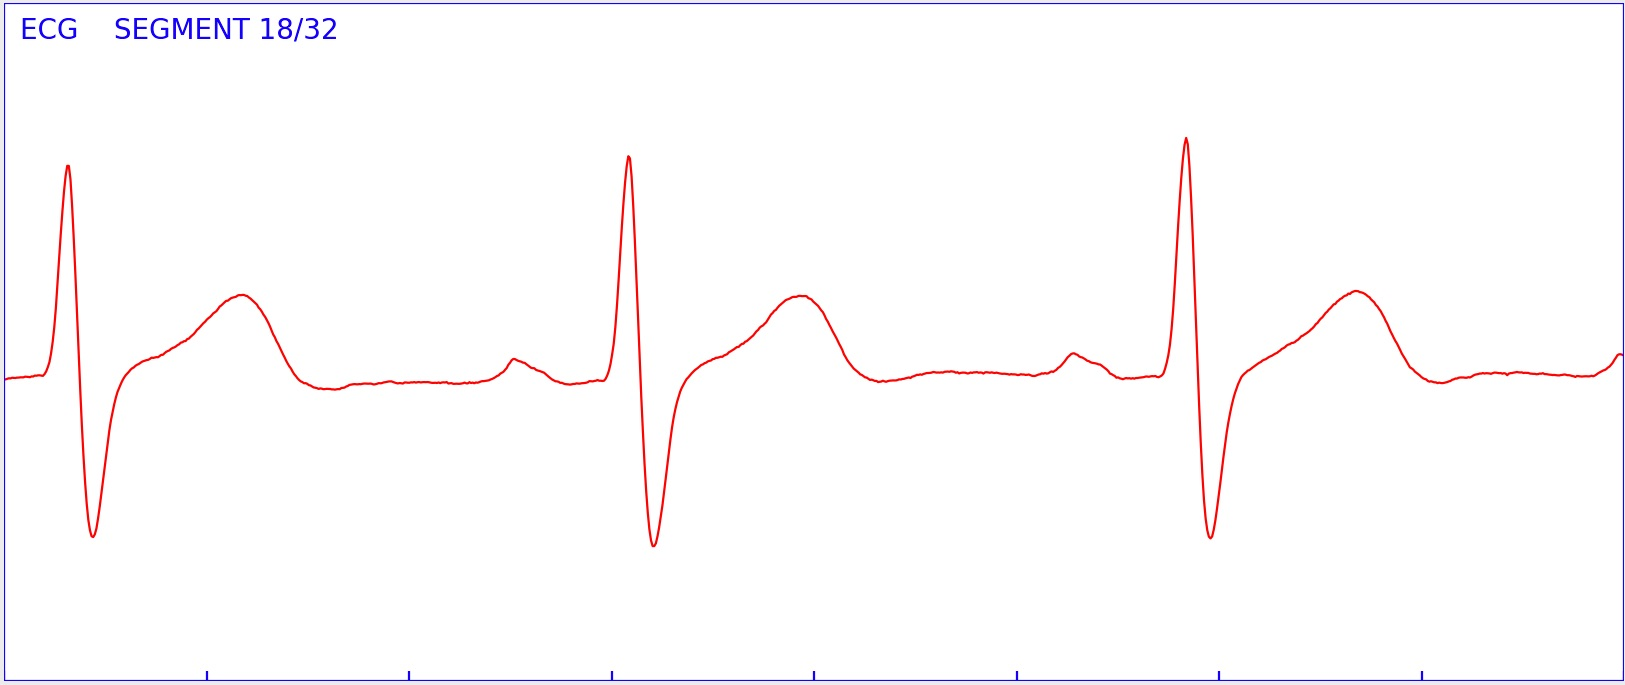
\includegraphics[scale=0.25]{img/artefact_1.jpeg}
    \par \vspace{0.25cm}
    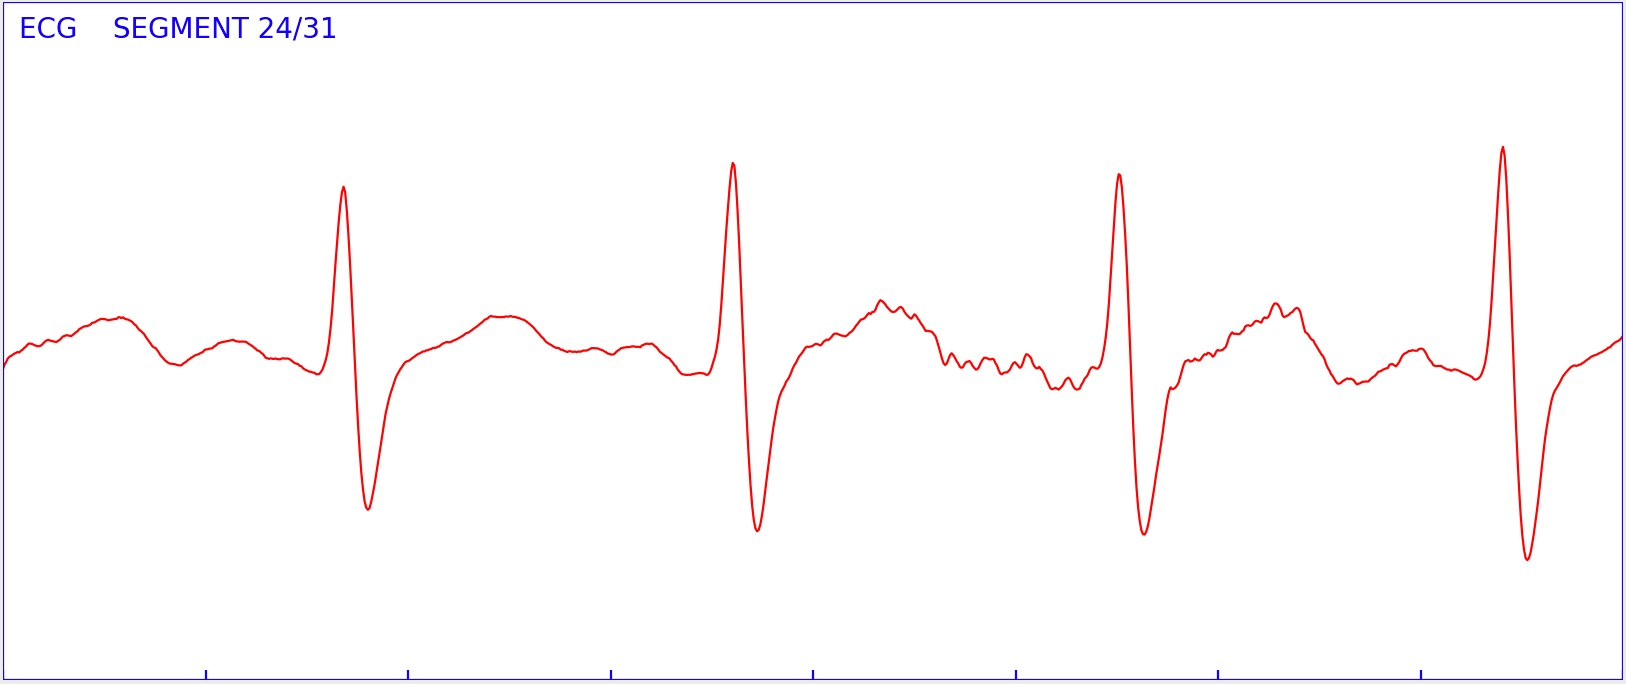
\includegraphics[scale=0.25]{img/artefact_1_1.jpeg}
    \caption{Segmenty patriace do kategórie 1.}
    \label{fig:artefact_1}
\end{figure}

\newpage

\subsection{Artefakt kategórie 2}

\textbf{Srdečný rytmus čitateľný} a aspoň jeden srdečný cyklus je čitateľný. Rušenie prítomné vo~všet-kých cykloch, amplitúda ani v jednom nepresahuje polovicu amplitúdy R-vlny.

\begin{figure}[H]
    \centering    
    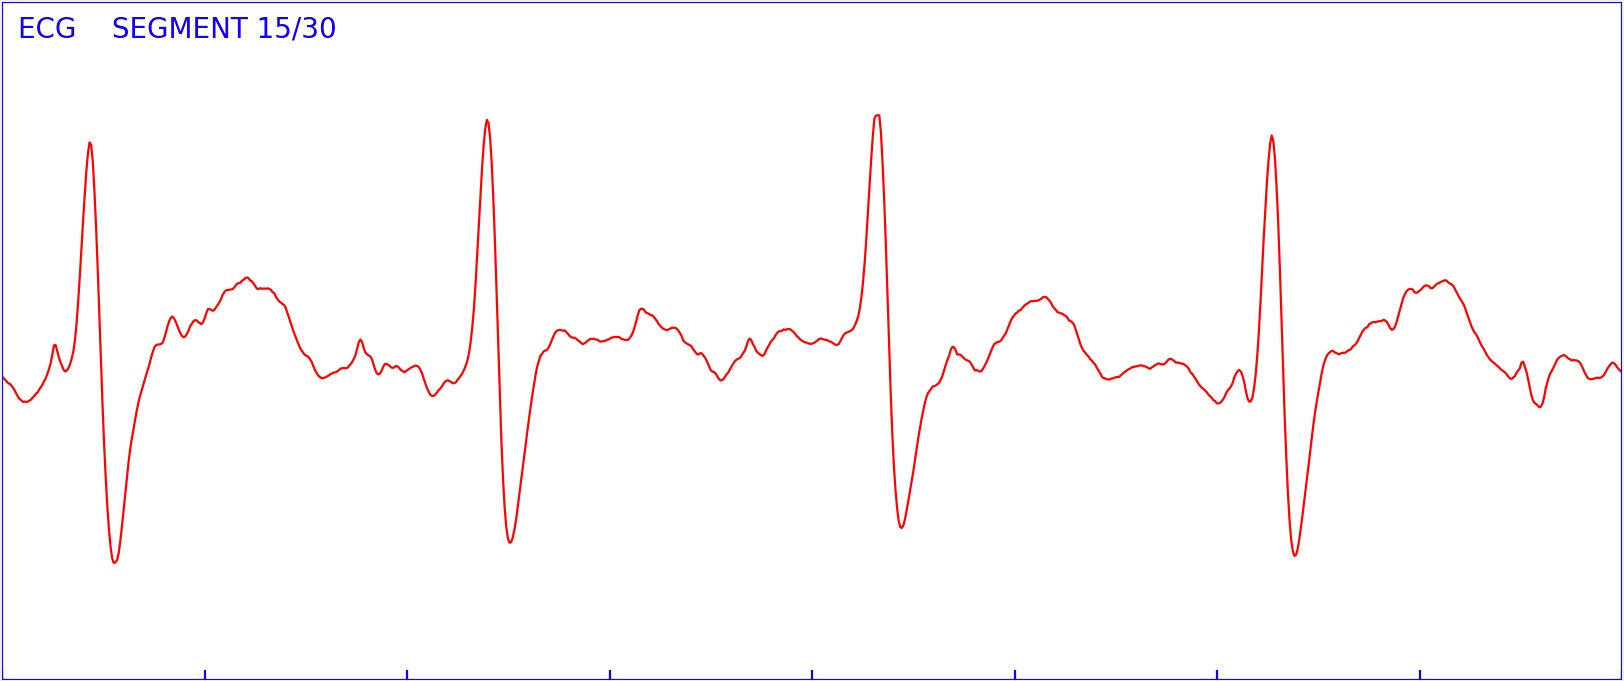
\includegraphics[scale=0.25]{img/artefact_2.jpeg}
    \caption{Segment patriaci do kategórie 2.}
    \label{fig:artefact_2}
\end{figure}

\subsection{Artefakt kategórie 3}

\textbf{Srdečný rytmus čitateľný} a zároveň ani jeden srdečný cyklus nie je čitateľný. Vznikajú falošné vlny, ktorých amplitúda presahuje polovicu amplitúdy R-vlny, často prítomné abrupty.

\begin{figure}[H]
    \centering    
    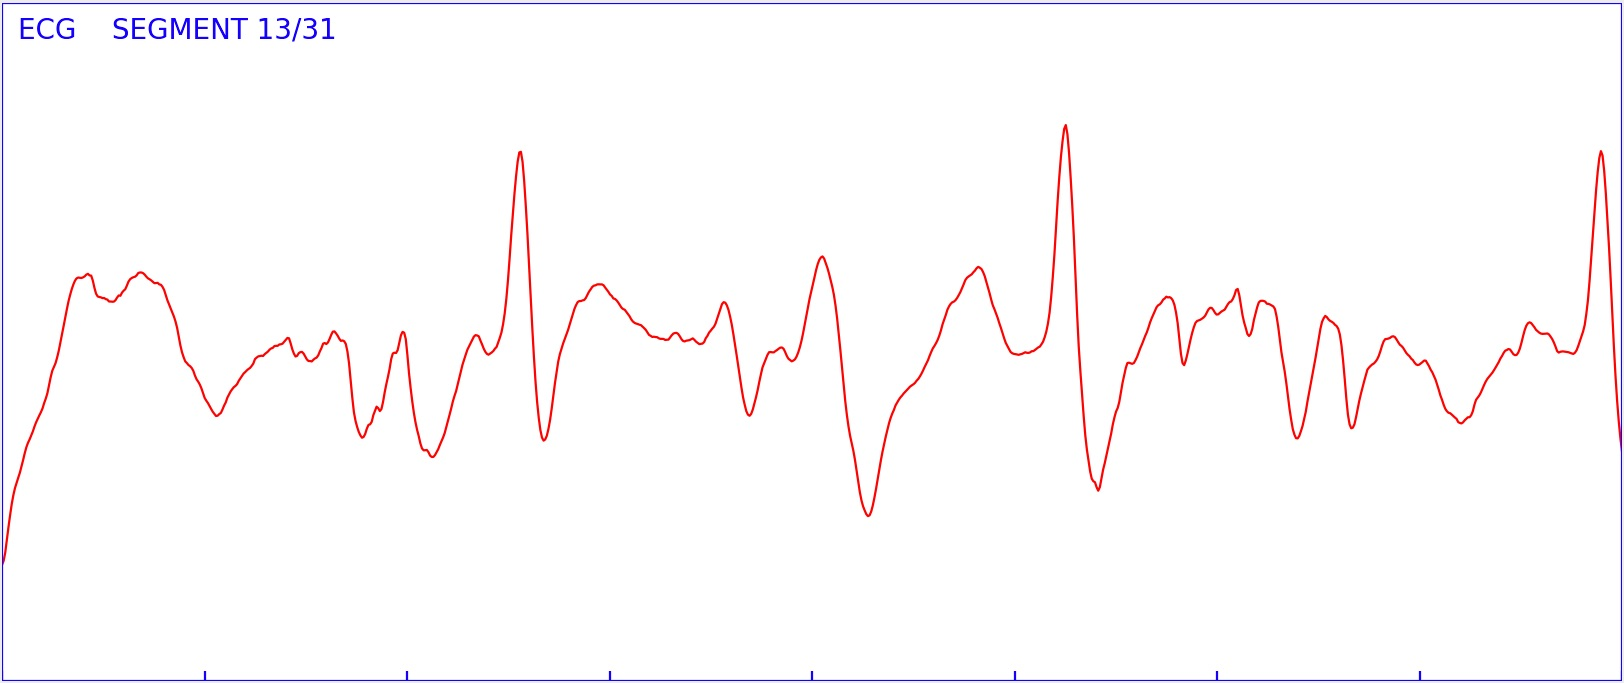
\includegraphics[scale=0.25]{img/artefact_3.jpeg}
    \caption{Segment patriaci do kategórie 3.}
    \label{fig:artefact_3}
\end{figure}

\newpage

\subsection{Artefakt kategórie 4}

Hlavným rozdielom oproti predošlým kategóriám je, že \textbf{srdečný rytmus nie je čitateľný}, prakticky sem spadajú dva rôzne prípady:

\begin{itemize}
    \item Na celom signáli je superponované rušenie s amplitúdou, ktorá znemožňuje aj kvalitnému QRS detektoru správnu detekciu R-vĺn. Vznikajú falošné vlny so zameniteľnou amplitúdou mimo refraktérnej fázy detektoru, teda v oblasti koniec T-vlny - začiatok Q-vlny (Obr. \ref{fig:artefact_4} hore).
    \item Aspoň jedna nerozoznateľná R-vlna, často kvôli saturácii signálu. Takýto segment je z hľadi-ska analýzy spektra ľahko zameniteľný s nižšími kategóriami, keďže rušenie nie je prítomné po celú dobu (Obr. \ref{fig:artefact_4} dole). 
\end{itemize}

\begin{figure}[H]
    \centering    
    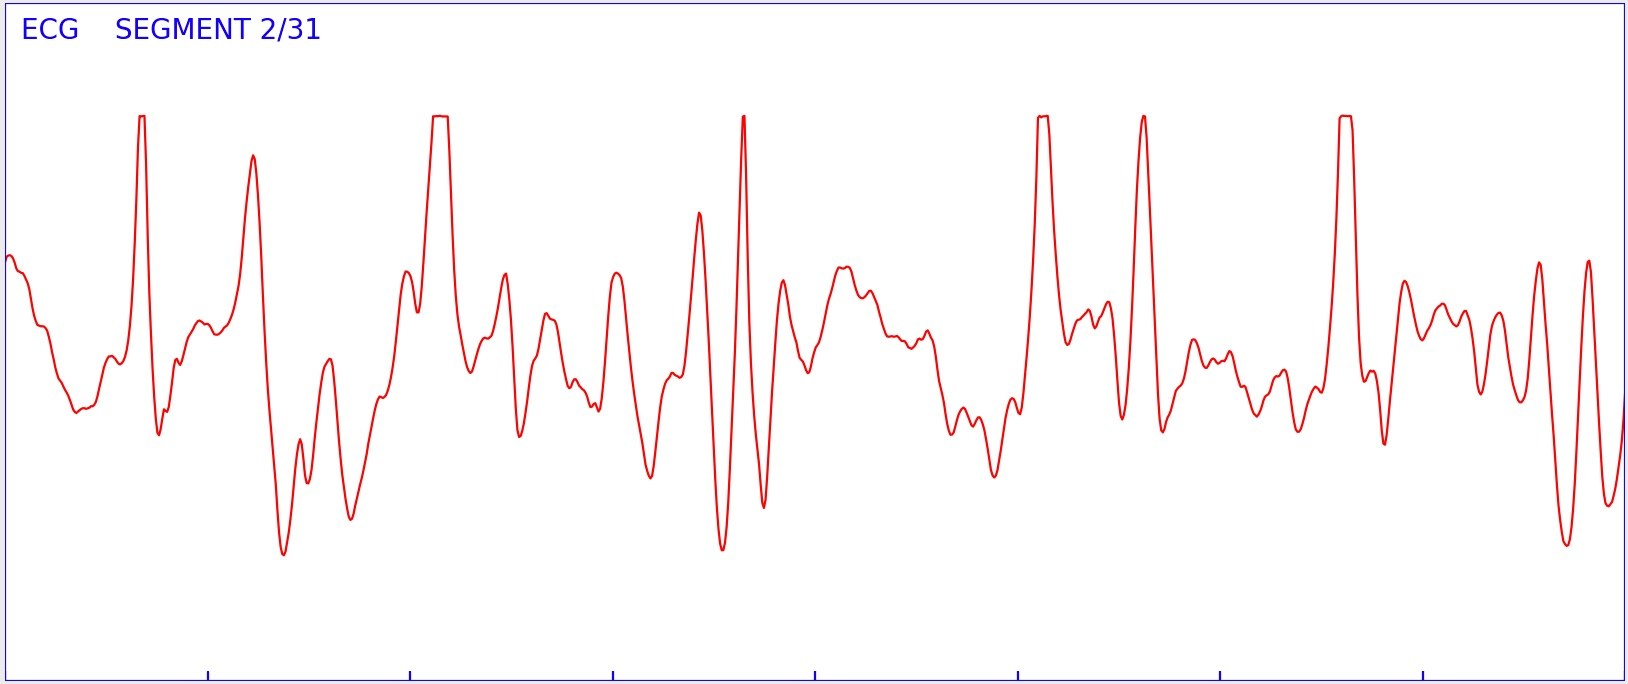
\includegraphics[scale=0.25]{img/artefact_4.jpeg}
    \par \vspace{0.25cm}
    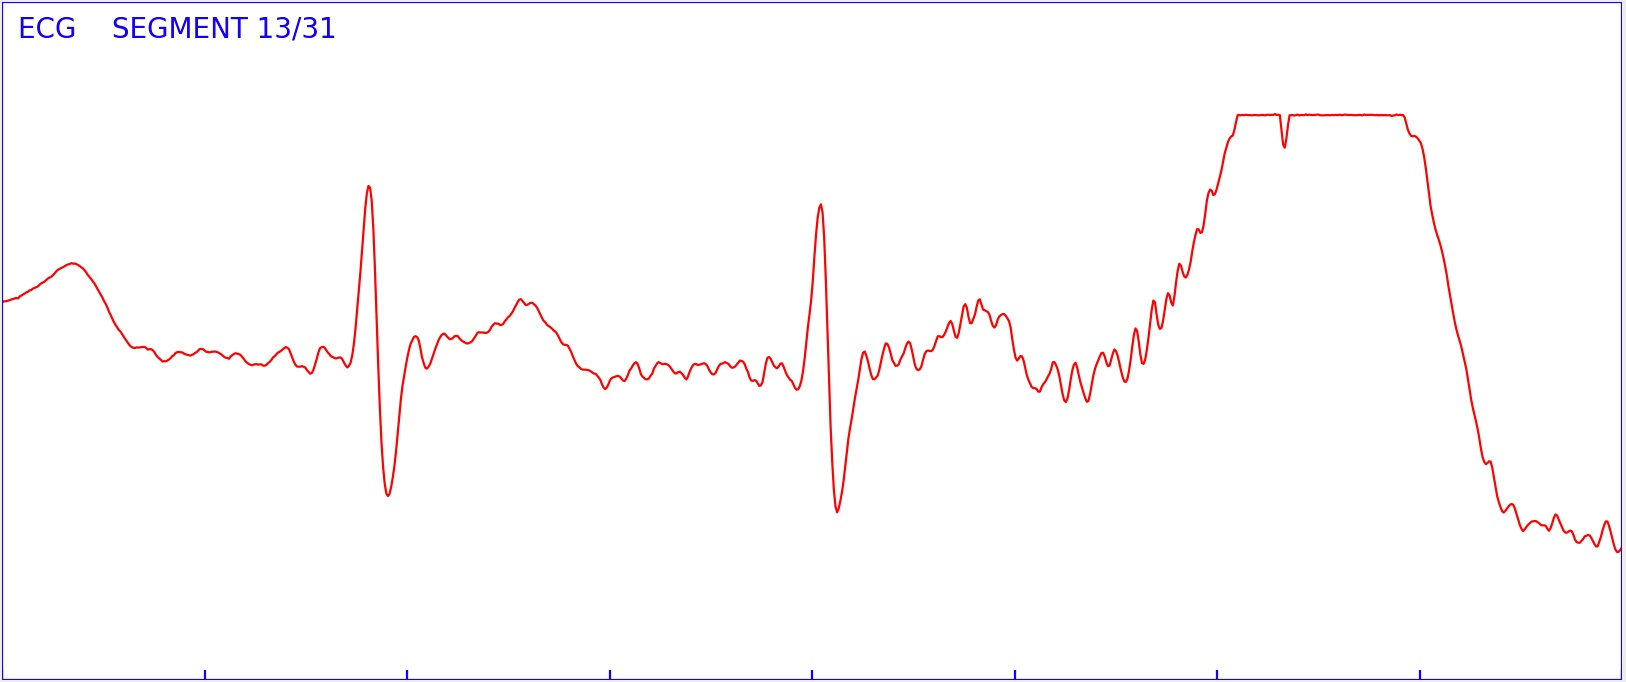
\includegraphics[scale=0.25]{img/artefact_4_1.jpeg}
    \caption{Segmenty patriace do kategórie 4.}
    \label{fig:artefact_4}
\end{figure}

\newpage


%---------------------------------------------------------------
\section{Štruktúra dát}
%---------------------------------------------------------------

EKG signál je zaznamenaný do súboru, ktorý obsahuje iba dva stĺpce - jeden pre časový údaj a~druhý pre hodnotu signálu v danom čase, jeho štruktúru je možné vidieť v tabuľke \ref{tab:input}. Prvý aj~druhý stĺpec obsahuje záznam vo forme časovej rady, v ukážke je zobrazených prvých 5 vzoriek záznamu.

\begin{table}[H]\centering
\caption[Súbor s EKG záznamom.]{~Súbor s EKG záznamom.}\label{tab:input}
    \begin{tabular}{c|c}
    	\textbf{timestamp} 	        & \textbf{value}   \tabularnewline \hline 
     	2024-03-26 15:04:53.249732  & 1698	           \tabularnewline \hline
     	2024-03-26 15:04:53.251727 	& 1874	           \tabularnewline \hline
        2024-03-26 15:04:53.253784 	& 2021	           \tabularnewline \hline
        2024-03-26 15:04:53.253784  & 2153	           \tabularnewline \hline
        2024-03-26 15:04:53.257780  & 2291	           \tabularnewline
    \end{tabular}
\end{table}

Pre správnu anotáciu typu pohybovej aktivity a zobrazenie druhu elektród v grafickom rozhraní je potrebné dodržať predpísané názvoslovie vstupného súboru, ktoré je \textit{ID\_TYP-ELEKTRÓDY\_TYP-AKTIVITY.csv}. Typ pohybovej aktivity je kódovaný podľa tabuľky \ref{tab:labels_activity}, pričom neznáma hodnota sa uvádza v prípade, že názov súboru na príslušnom mieste neobsahuje ani jednu z uvedených aktivít. Typ použitých elektród je kódovaný podľa tabuľky \ref{tab:labels_electrode}.

\begin{table}[H]\centering
\caption[Kódovanie pohybovej aktivity.]{~Kódovanie pohybovej aktivity.}\label{tab:labels_activity}
    \begin{tabular}{l|c}
    	\textbf{Pohybová aktivita}  & \textbf{Číselná hodnota}    \tabularnewline \hline 
     	Kľudová fáza                & 0	                          \tabularnewline \hline
     	Pohyby hornými končatinami 	& 1	                          \tabularnewline \hline
        Chôdza 4 km/h 	            & 2	                          \tabularnewline \hline
        Beh 8 km/h                  & 3	                          \tabularnewline \hline
        Drepy                       & 4	                          \tabularnewline \hline
        Neznáma                     & -1                          \tabularnewline
    \end{tabular}
\end{table}

\begin{table}[H]\centering
\caption[Kódovanie typu elektród.]{~Kódovanie typu elektród.}\label{tab:labels_electrode}
    \begin{tabular}{l|c}
    	\textbf{Typ elektród}  & \textbf{Číselná hodnota}     \tabularnewline \hline 
     	Ag/AgCl                & 1	                          \tabularnewline \hline
     	Chróm-niklel	       & 2	                          \tabularnewline \hline
        Textil	               & 3	                          \tabularnewline \hline
        Neznámy	               & -1	                          \tabularnewline
    \end{tabular}
\end{table}

Názvoslovie súborov vytvorených pomocou grafického rozhrania na anotáciu dát je~nasledovné - \textit{ID\_TYP-ELEKTRÓDY\_TYP-AKTIVITY\_DĹŽKA-SEGMENTU.csv}. Dĺžka segmentu je v názve uvedená aby sa dali odlíšiť anotácie vstupných súborov pre rôzne zvolené dĺžky segmentu. Súbory obsahujú stĺpec pre začiatočnú a koncovú pozíciu segmentu, typ aktivity, artefakt a typ elektródy, ich štruktúra je zobrazená v tabuľke \ref{tab:output}. 

\begin{table}[H]\centering
\caption[Výstupný súbor s anotovanými dátami.]{~Výstupný súbor s anotovanými dátami.}\label{tab:output}
    \begin{tabular}{c|c|c|c|c}
    	\textbf{start} & \textbf{end} & \textbf{activity} & \textbf{artefact} & \textbf{electrode} \tabularnewline \hline 
     	0		       & 1000		  & 1	              & 1	              & 1	               \tabularnewline \hline
     	1000	       & 2000	      & 1	              & 1	              & 1	               \tabularnewline \hline
        2000	       & 3000	      & 1	              & 2	              & 1	               \tabularnewline \hline
        3000	       & 4000	      & 1	              & 2	              & 1	               \tabularnewline \hline
        4000	       & 5000	      & 1	              & 3	              & 1	               \tabularnewline \hline
        5000	       & 6000	      & 1	              & 4	              & 1	               \tabularnewline
    \end{tabular}
\end{table}


%---------------------------------------------------------------
\section{Zastúpenie tried}
%---------------------------------------------------------------

Po rozdelení surových dát na 2-sekundové segmenty sme dostali konečnú veľkosť dátovej sady - \textbf{4602 segmentov}. Keďže nevyvážené zastúpenie tried v dátovej sade môže mať vplyv na~výsledky klasifikácie, v krátkosti sme sa pozreli na ich distribúciu. Z hľadiska tried pohybových artefaktov je dátová sada výrazne nevyvážená, pričom s narastajúcou intenzitou artefaktu zastúpenie tried klesá. Celkové počty segmentov patriacich do jednotlivých kategórií je možné vidieť na grafe \ref{fig:artefact_stats}. 

\begin{figure}[H]
    \centering    
    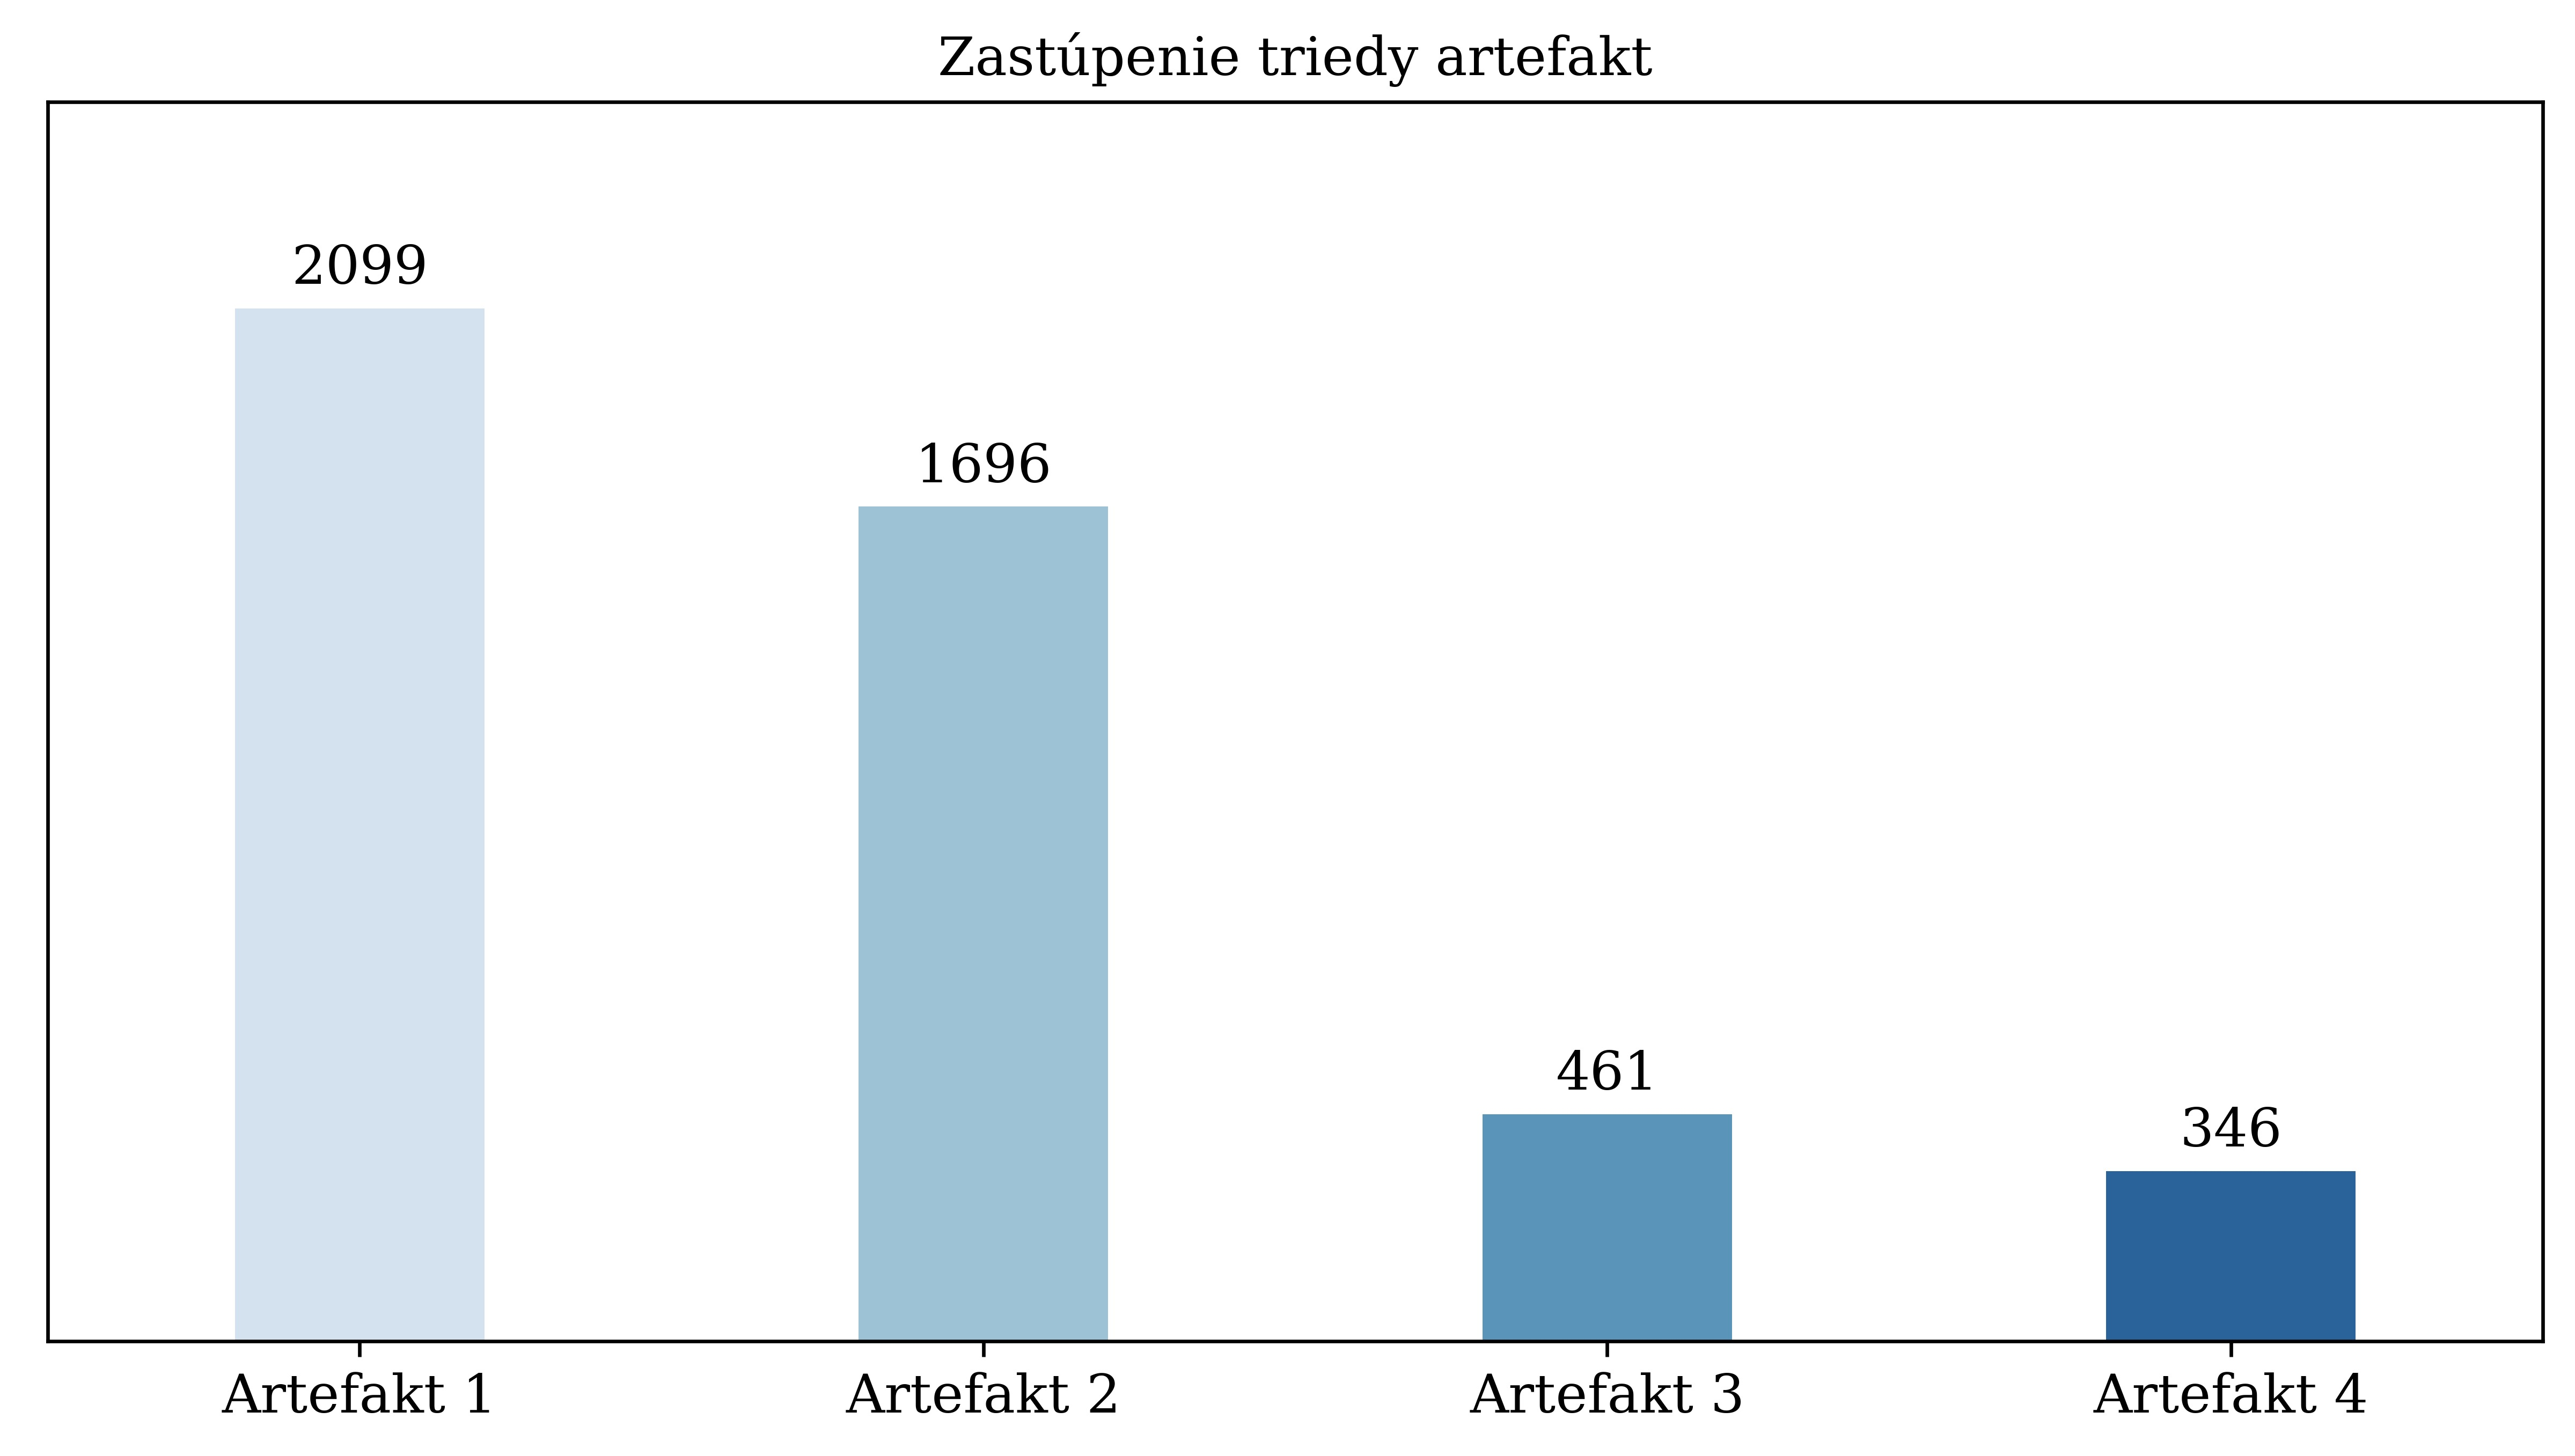
\includegraphics[scale=0.07]{img/artefact_stats.jpg}
    \caption{Počty segmentov podľa typu artefaktu.}
    \label{fig:artefact_stats}
\end{figure}

Z hľadiska výskytu rôznych aktivít a elektród je dátová sada vyvážená, čo vyplýva zo~samotnej metodiky experimentu. Pre každý subjekt boli zaznamenané všetky typy aktivít po~dobu približne jednej minúty, pomocou troch rôznych druhov elektród, čím sme zaistili rovnomernú distribúciu týchto tried. Konkrétne počty segmentov pre jednotlivé typy aktivít je možné vidieť na grafe \ref{fig:activity_stats} a pre typy elektród na grafe \ref{fig:electrode_stats}.

\begin{figure}[H]
    \centering    
    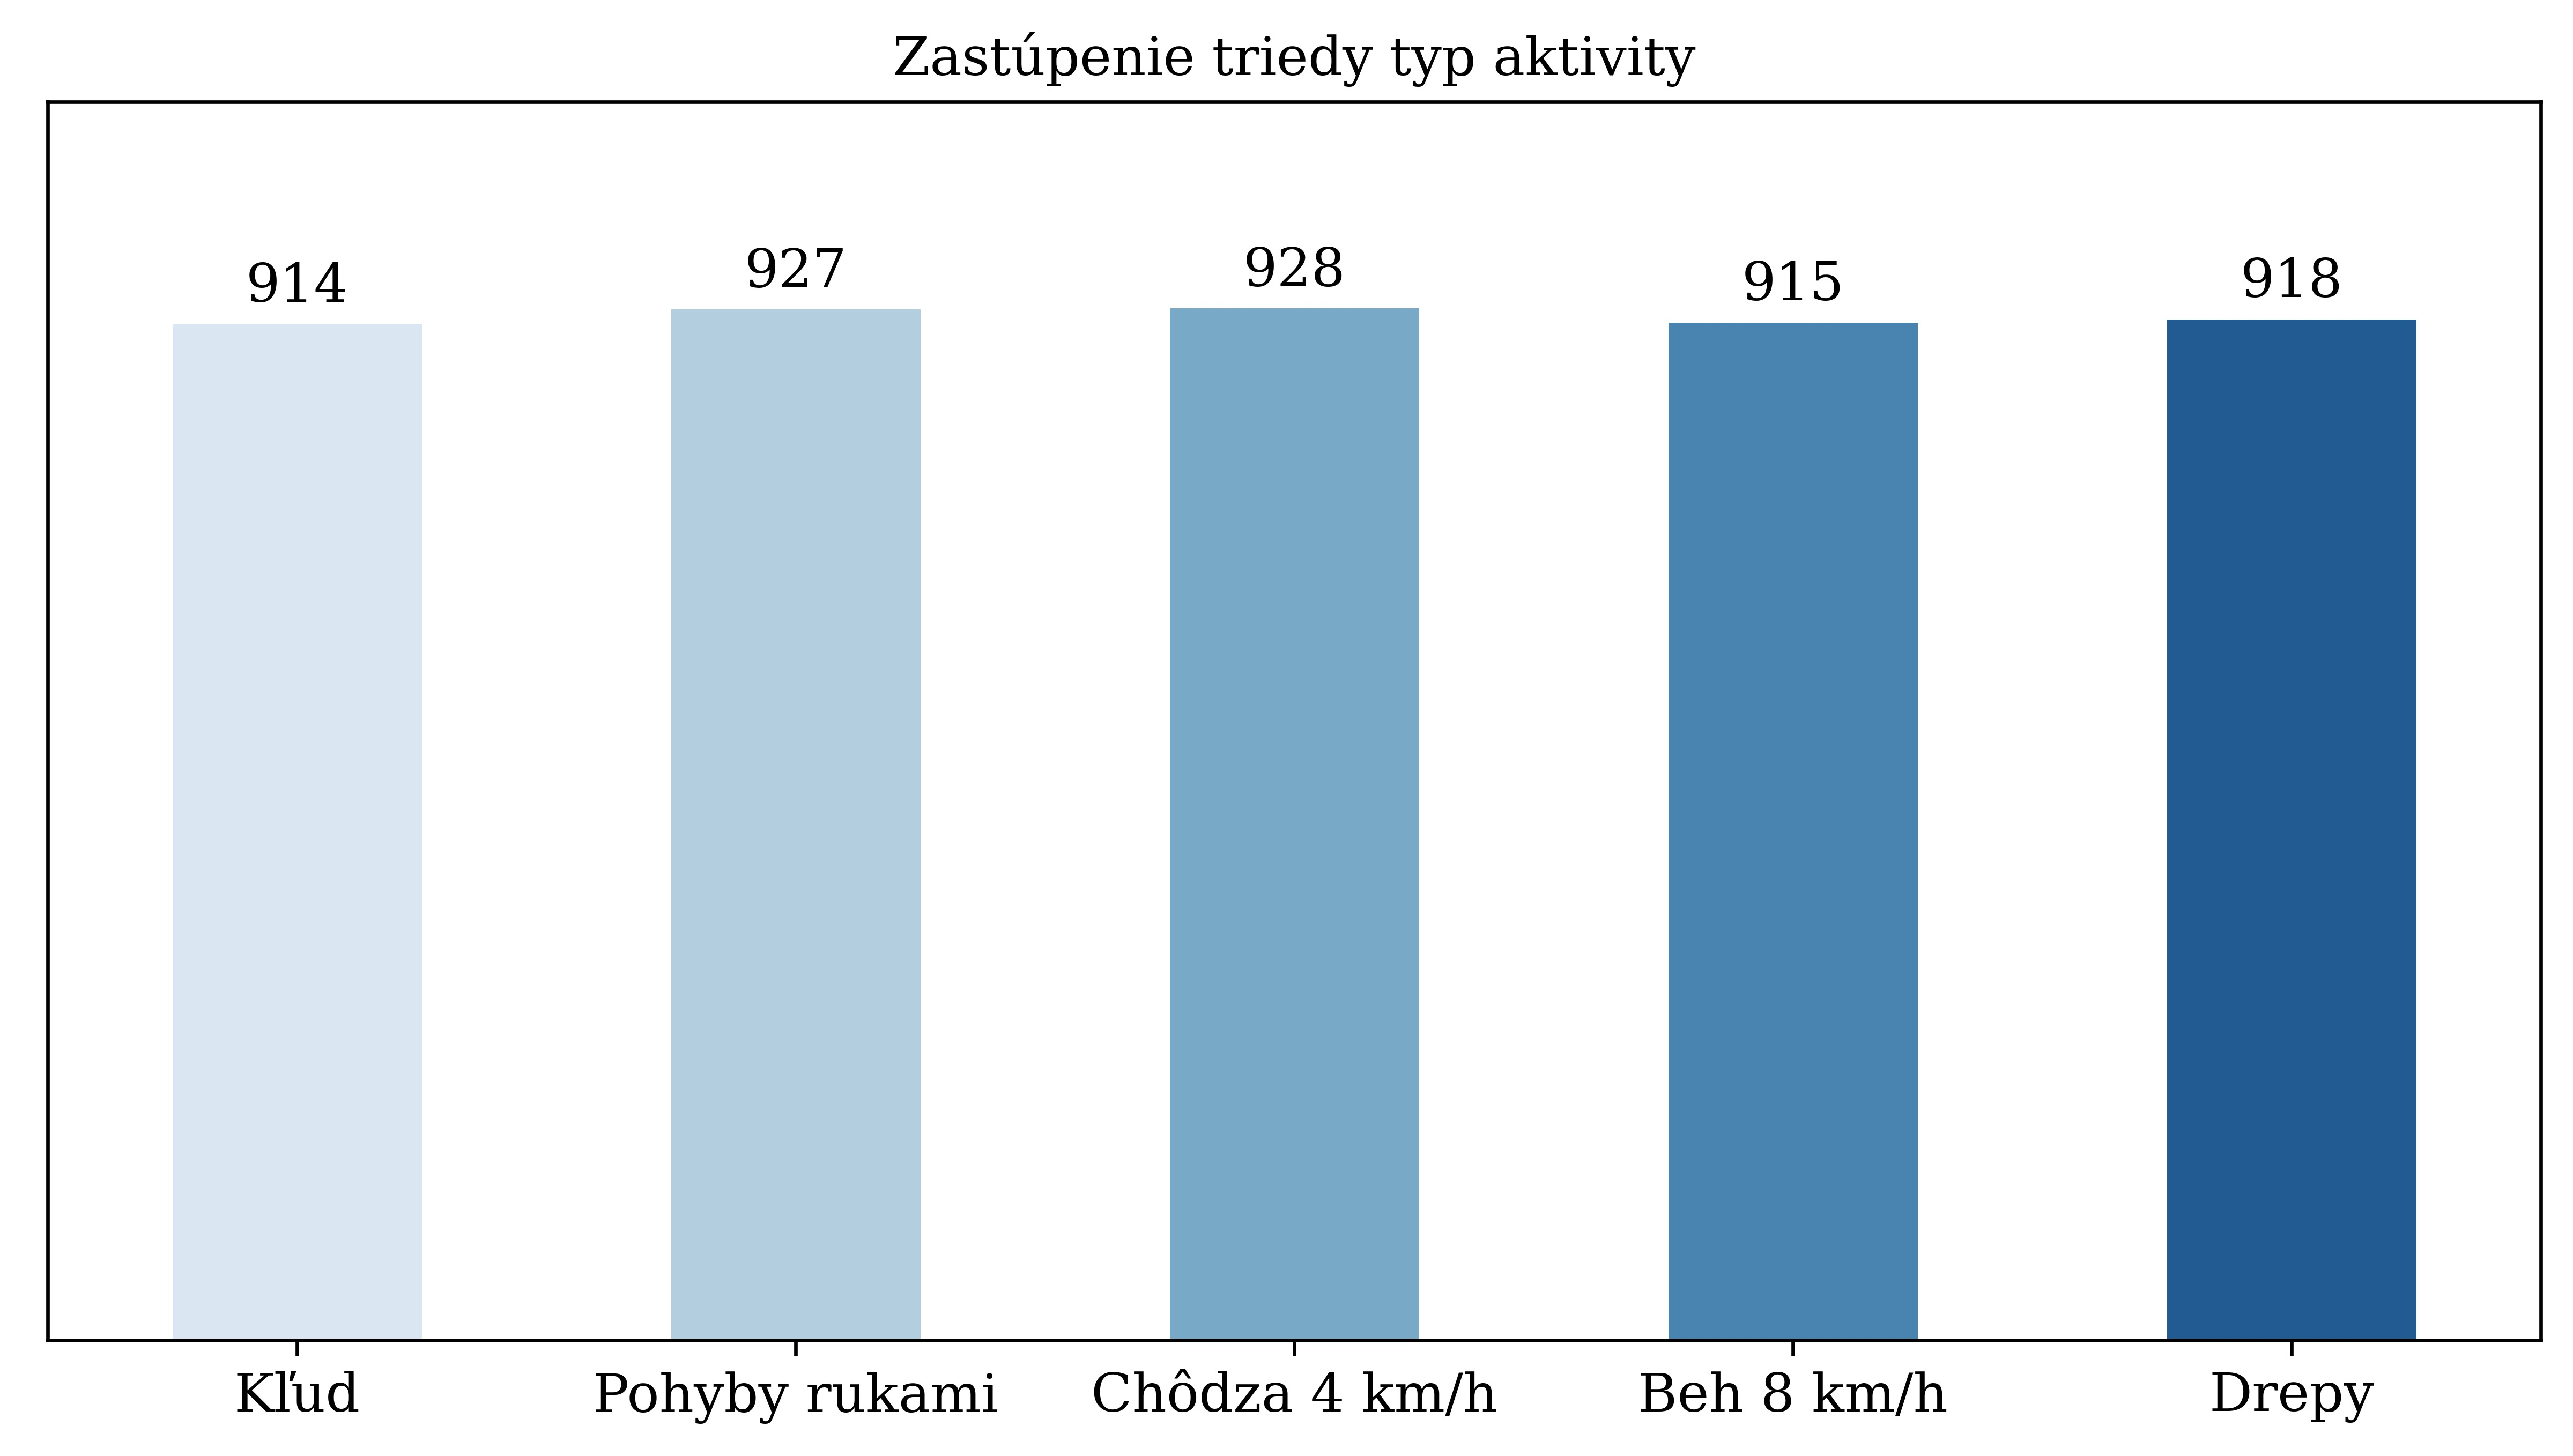
\includegraphics[scale=0.07]{img/activity_stats.jpg}
    \caption{Počty segmentov podľa typu aktivity.}
    \label{fig:activity_stats}
\end{figure}

\begin{figure}[H]
    \centering    
    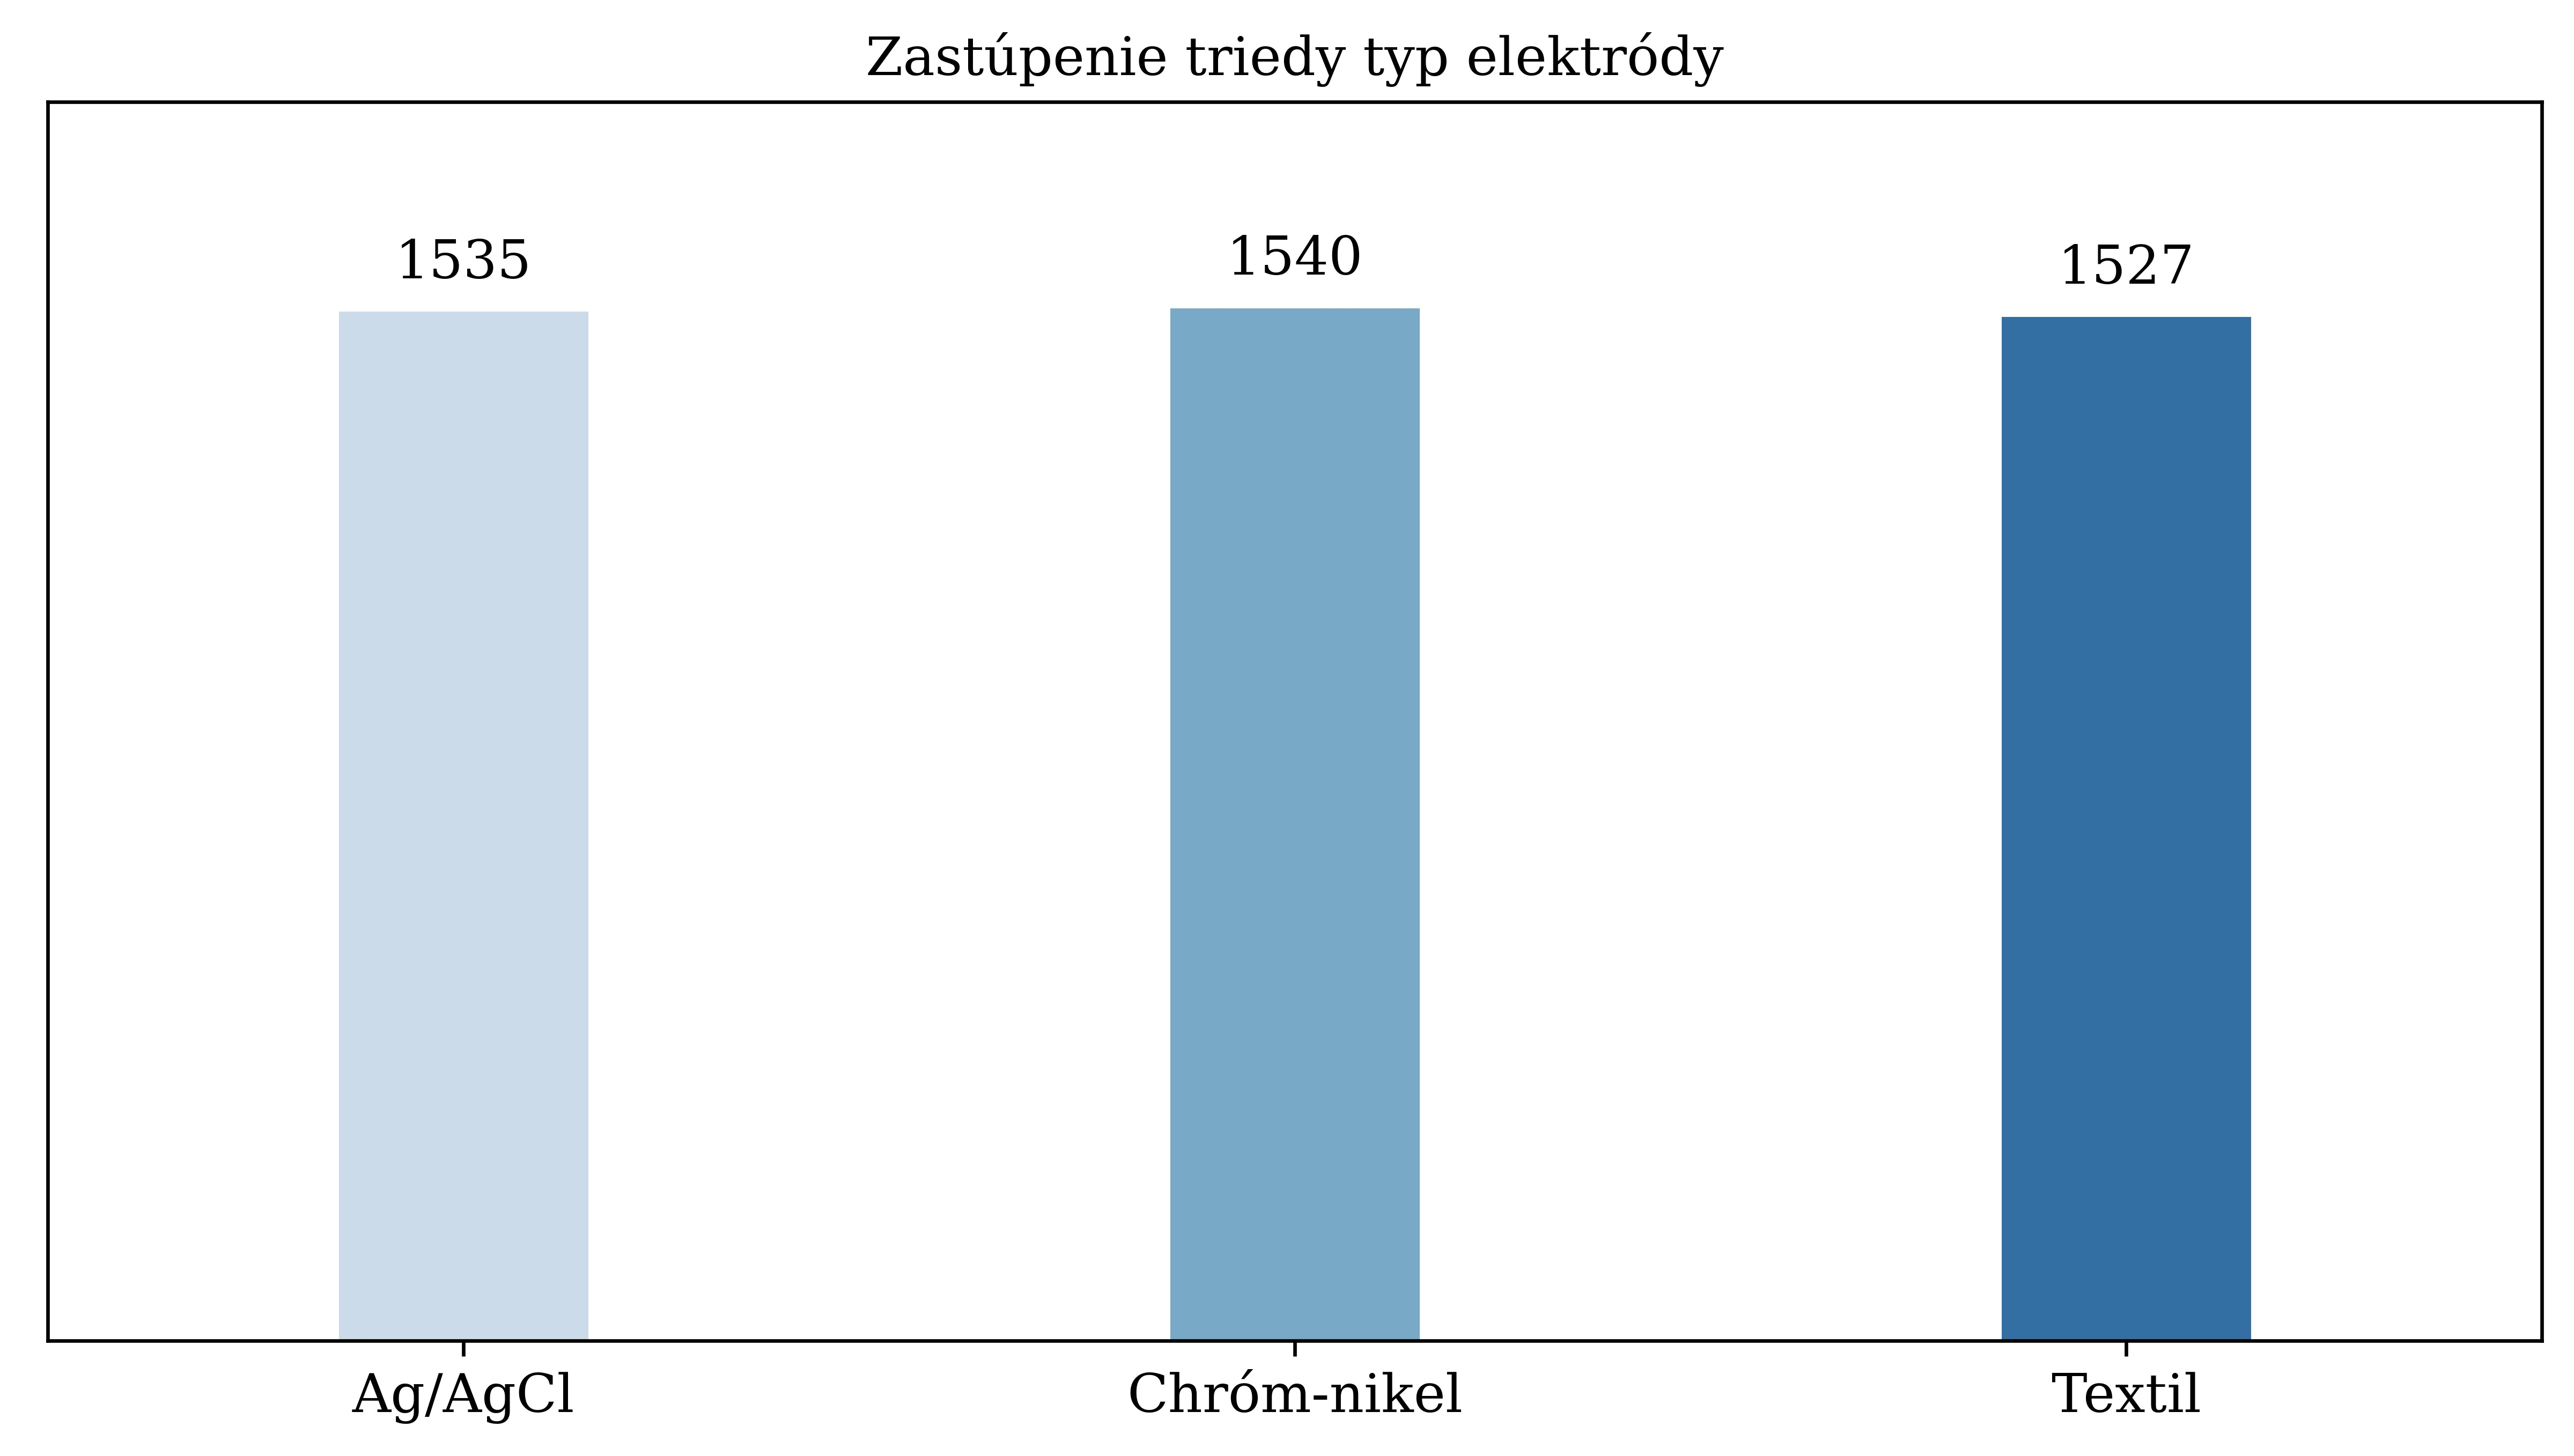
\includegraphics[scale=0.07]{img/electrode_stats.jpg}
    \caption{Počty segmentov podľa typu elektródy.}
    \label{fig:electrode_stats}
\end{figure}


%---------------------------------------------------------------
\section{Predspracovanie dát}
%---------------------------------------------------------------

Keďže jedným z cieľov práce je nájsť riešenie na rozpoznávanie pohybových artefaktov také, aby bolo využiteľné v reálnom čase, jednou z požiadaviek na riešenie je rýchle spracovanie analyzovaného segmentu. Preto sme v rámci predspracovania dát pristúpili iba k normalizácii - tá~je~nevyhnutná, ak chceme, aby bol model využiteľný aj na dáta namerané iným snímačom, ktorý nemusí nutne disponovať rovnakým AD prevodníkom. Keďže poskytnutý nositeľný snímač EKG využíva 12 bitový AD prevodník, dáta boli normalizované na rozsah 0 až 4095. Následne bola z~normalizovaných EKG záznamov pre každý segment pomocou rýchlej Fourierovej transformácie extrahovaná frekvenčná zložka v podobe amplitúdového spektra.


%---------------------------------------------------------------
\chapter{Výsledky}
%---------------------------------------------------------------

Kapitola je členená podľa jednotlivých dielčích výstupov práce. Na začiatok sa v krátkosti pozrieme na vyhodnotenie typov elektród a ich vhodnosť na terénne monitorovanie, následne výsledky klasifikácie aktivít, a na záver sa pozrieme na hlavný výstup práce a to výsledky klasifikácie pohybových artefaktov. Všetky modely boli implementované pomocou voľne dostupnej knižnice \textbf{Keras}\footnote{https://keras.io}, ktorá beží nad knižnicou \textbf{TensorFlow}\footnote{https://www.tensorflow.org} a poskytuje rozhranie na tvorbu a~trénovanie modelov strojového učenia v jazyku Python. Trénovanie prebiehalo lokálne na stroji MacBook Pro 2019 s procesorom 2,4 GHz Quad-Core Intel Core i5 a 16 GB LPDDR3 RAM pamäťou. Na sledovanie výsledkov sme využili nástroj \textbf{Neptune}\footnote{https://neptune.ai}, ktorý poskytuje grafické rozhranie na zaznamenávanie priebehu trénovania v reálnom čase.

\section{Vyhodnotenie typu elektród}

\begin{table}[H]\centering
\catcode`\-=12
\caption[Podiel artefaktov podľa typu aktivity a typu elektródy.]{~Podiel artefaktov podľa typu aktivity a typu elektródy.}\label{tab:electrode_stats}
    \begin{tabular}{l C{2.5em}|C{2.5em}|C{2.5em}|C{2.5em}}

        \multicolumn{1}{c}{} & \multicolumn{4}{c}{\textbf{Kľud}} \\
        \cline{2-5}
        \multicolumn{1}{c}{} & \multicolumn{1}{c|}{\textbf{1}} & \textbf{2} & \textbf{3} & \textbf{4} \\
        \cline{2-5}  
        \textbf{Ag/AgCl} & 99,7 & 0,0 & 0,0 & 0,3 \\
        \cline{2-5}
        \textbf{Chróm-nikel} & 99,7 & 0,3 & 0,0 & 0,0 \\
        \cline{2-5}
        \textbf{Textil} & 100,0 & 0,0 & 0,0 & 0,0 \\

    \end{tabular}

    \par \vspace{0.5cm}
    
    \begin{tabular}{lC{2.5em}|C{2.5em}|C{2.5em}|C{2.5em}||C{2.5em}|C{2.5em}|C{2.5em}|C{2.5em}}

        \multicolumn{1}{c}{} & \multicolumn{4}{c}{\textbf{Ruky}} & \multicolumn{4}{c}{\textbf{Chôdza}} \\
        \cline{2-9}
        \multicolumn{1}{c}{} & \textbf{1} & \textbf{2} & \textbf{3} & \textbf{4} & \textbf{1} & \textbf{2} & \textbf{3} & \textbf{4} \\
        \cline{2-9}  
        \textbf{Ag/AgCl} & \textbf{23,3} & 76,4 & 0,0 & \textbf{0,3} & 20,1 & 32,0 & 20,7 & 27,2 \\
        \cline{2-9}
        \textbf{Chróm-nikel} & 16,8 & 80,3 & 0,0 & 2,9 & 79,7 & 19,3 & 0,0 & 1,0 \\
        \cline{2-9}
        \textbf{Textil} & 14,9 & 65,0 & 7,8 & 12,3 & \textbf{98,7} & 0,7 & 0,0 & \textbf{0,6} \\

    \end{tabular}
\end{table}

\begin{table}[H]\centering
\catcode`\-=12
    \par \vspace{0.5cm}

    \begin{tabular}{lC{2.5em}|C{2.5em}|C{2.5em}|C{2.5em}||C{2.5em}|C{2.5em}|C{2.5em}|C{2.5em}}

        \multicolumn{1}{c}{} & \multicolumn{4}{c}{\textbf{Beh}} & \multicolumn{4}{c}{\textbf{Drepy}} \\
        \cline{2-9}
        \multicolumn{1}{c}{} & \textbf{1} & \textbf{2} & \textbf{3} & \textbf{4} & \textbf{1} & \textbf{2} & \textbf{3} & \textbf{4} \\
        \cline{2-9}
        \textbf{Ag/AgCl} & 0,0 & 10,2 & 39,3 & 50,5 & \textbf{48,7} & 41,6 & 9,7 & \textbf{0,0} \\
        \cline{2-9}
        \textbf{Chróm-nikel} & 0,0 & 57,7 & 30,6 & 11,7 & 36,8 & 57,0 & 3,3 & 2,9 \\
        \cline{2-9}
        \textbf{Textil} & 0,0 & \textbf{69,5} & 28,5 & \textbf{2,0} & 46,2 & 41,6 & 10,9 & 1,3 \\

    \end{tabular}
\end{table}

V tabuľke \ref{tab:electrode_stats} môžeme vidieť percentuálny podiel tried pohybových artefaktov, pre jednotlivé typy elektród, rozdelený podľa aktivít. V kľudovej fáze boli takmer všetky segmenty s~výnimkou dvoch klasifikované ako obsahujúce minimálne až žiadne rušenie. Pri pohybe hornými končatinami a drepoch a meraním pomocou Ag/AgCl elektród bol najväčší podiel segmentov klasifikovaný ako trieda 1 (23,3 \% pri pohybe hornými končatinami a 48,7 \% pri drepoch) a najmenší podiel ako~trieda 4 (0,3 \% pri pohybe hornými končatinami a 0,0 \% pri drepoch), kvôli čomu dopadli spomedzi testovaných elektród najlepšie. Dôvodom je pravdepodobne to, že tieto elektródy sú~priamo nalepené na koži, narozdiel od ostatných dvoch, ktoré sú upevnené pásom - vďaka tomu sa vedia lepšie vysporiadať s pohybmi v trupe.

Pri textilných elektródach a pohybových aktivitách chôdza a beh bol najväčší podiel segmentov klasifikovaný ako trieda 1 prípadne 2 (98,7 \% pri chôdzi a 69,5 \% pri behu) a najmenší podiel ako trieda 4 (0,6 \% pri chôdzi a 2,0 \% pri behu). Ani jeden segment obsahujúci záznam behu nebol klasifikovaný ako trieda 1, čo znamená, že tento typ aktivity je najnáročnejší na~správne zachytenie. V prípade behu a chôdze vzniknuté artefakty nie sú spôsobené pohybom v~oblasti trupu, ale prevažne rytmickými nárazmi. Zatiaľ čo rozdiel medzi jednotlivými elektródami pri~pohybe hornými končatinami a drepoch nebol až taky výrazný, Ag/AgCl elektródy pri chôdzi a~behu zaostávajú o desiatky percent, čo má veľký vplyv na finálne výsledky.

Na grafe \ref{fig:electrode_stats_2} môžeme vidieť celkové výsledky, v ktorých si Ag/AgCl elektródy výrazne pohoršili a dopadli viditeľne najhoršie - najnižší podiel segmentov bol klasifikovaný ako trieda 1 a najvyšší ako trieda 4. V oboch prípadoch ide o rozdiel väčší ako 10 \% oproti ostatným dvom typom elektród. Chróm-niklové a textilné elektródy dopadli podobne, pričom textilné elektródy dosiahli lepší výsledok pri triede 1, kde predbehli chróm-niklové o 5,3 \%. Z porovnania elektród vyplýva, že najodolnejšie voči pohybovým artefaktom sú textilné elektródy, pričom práve tento typ hodnotili aj subjekty experimentu ako najkomfortnejší.

\begin{figure}[H]
    \centering    
    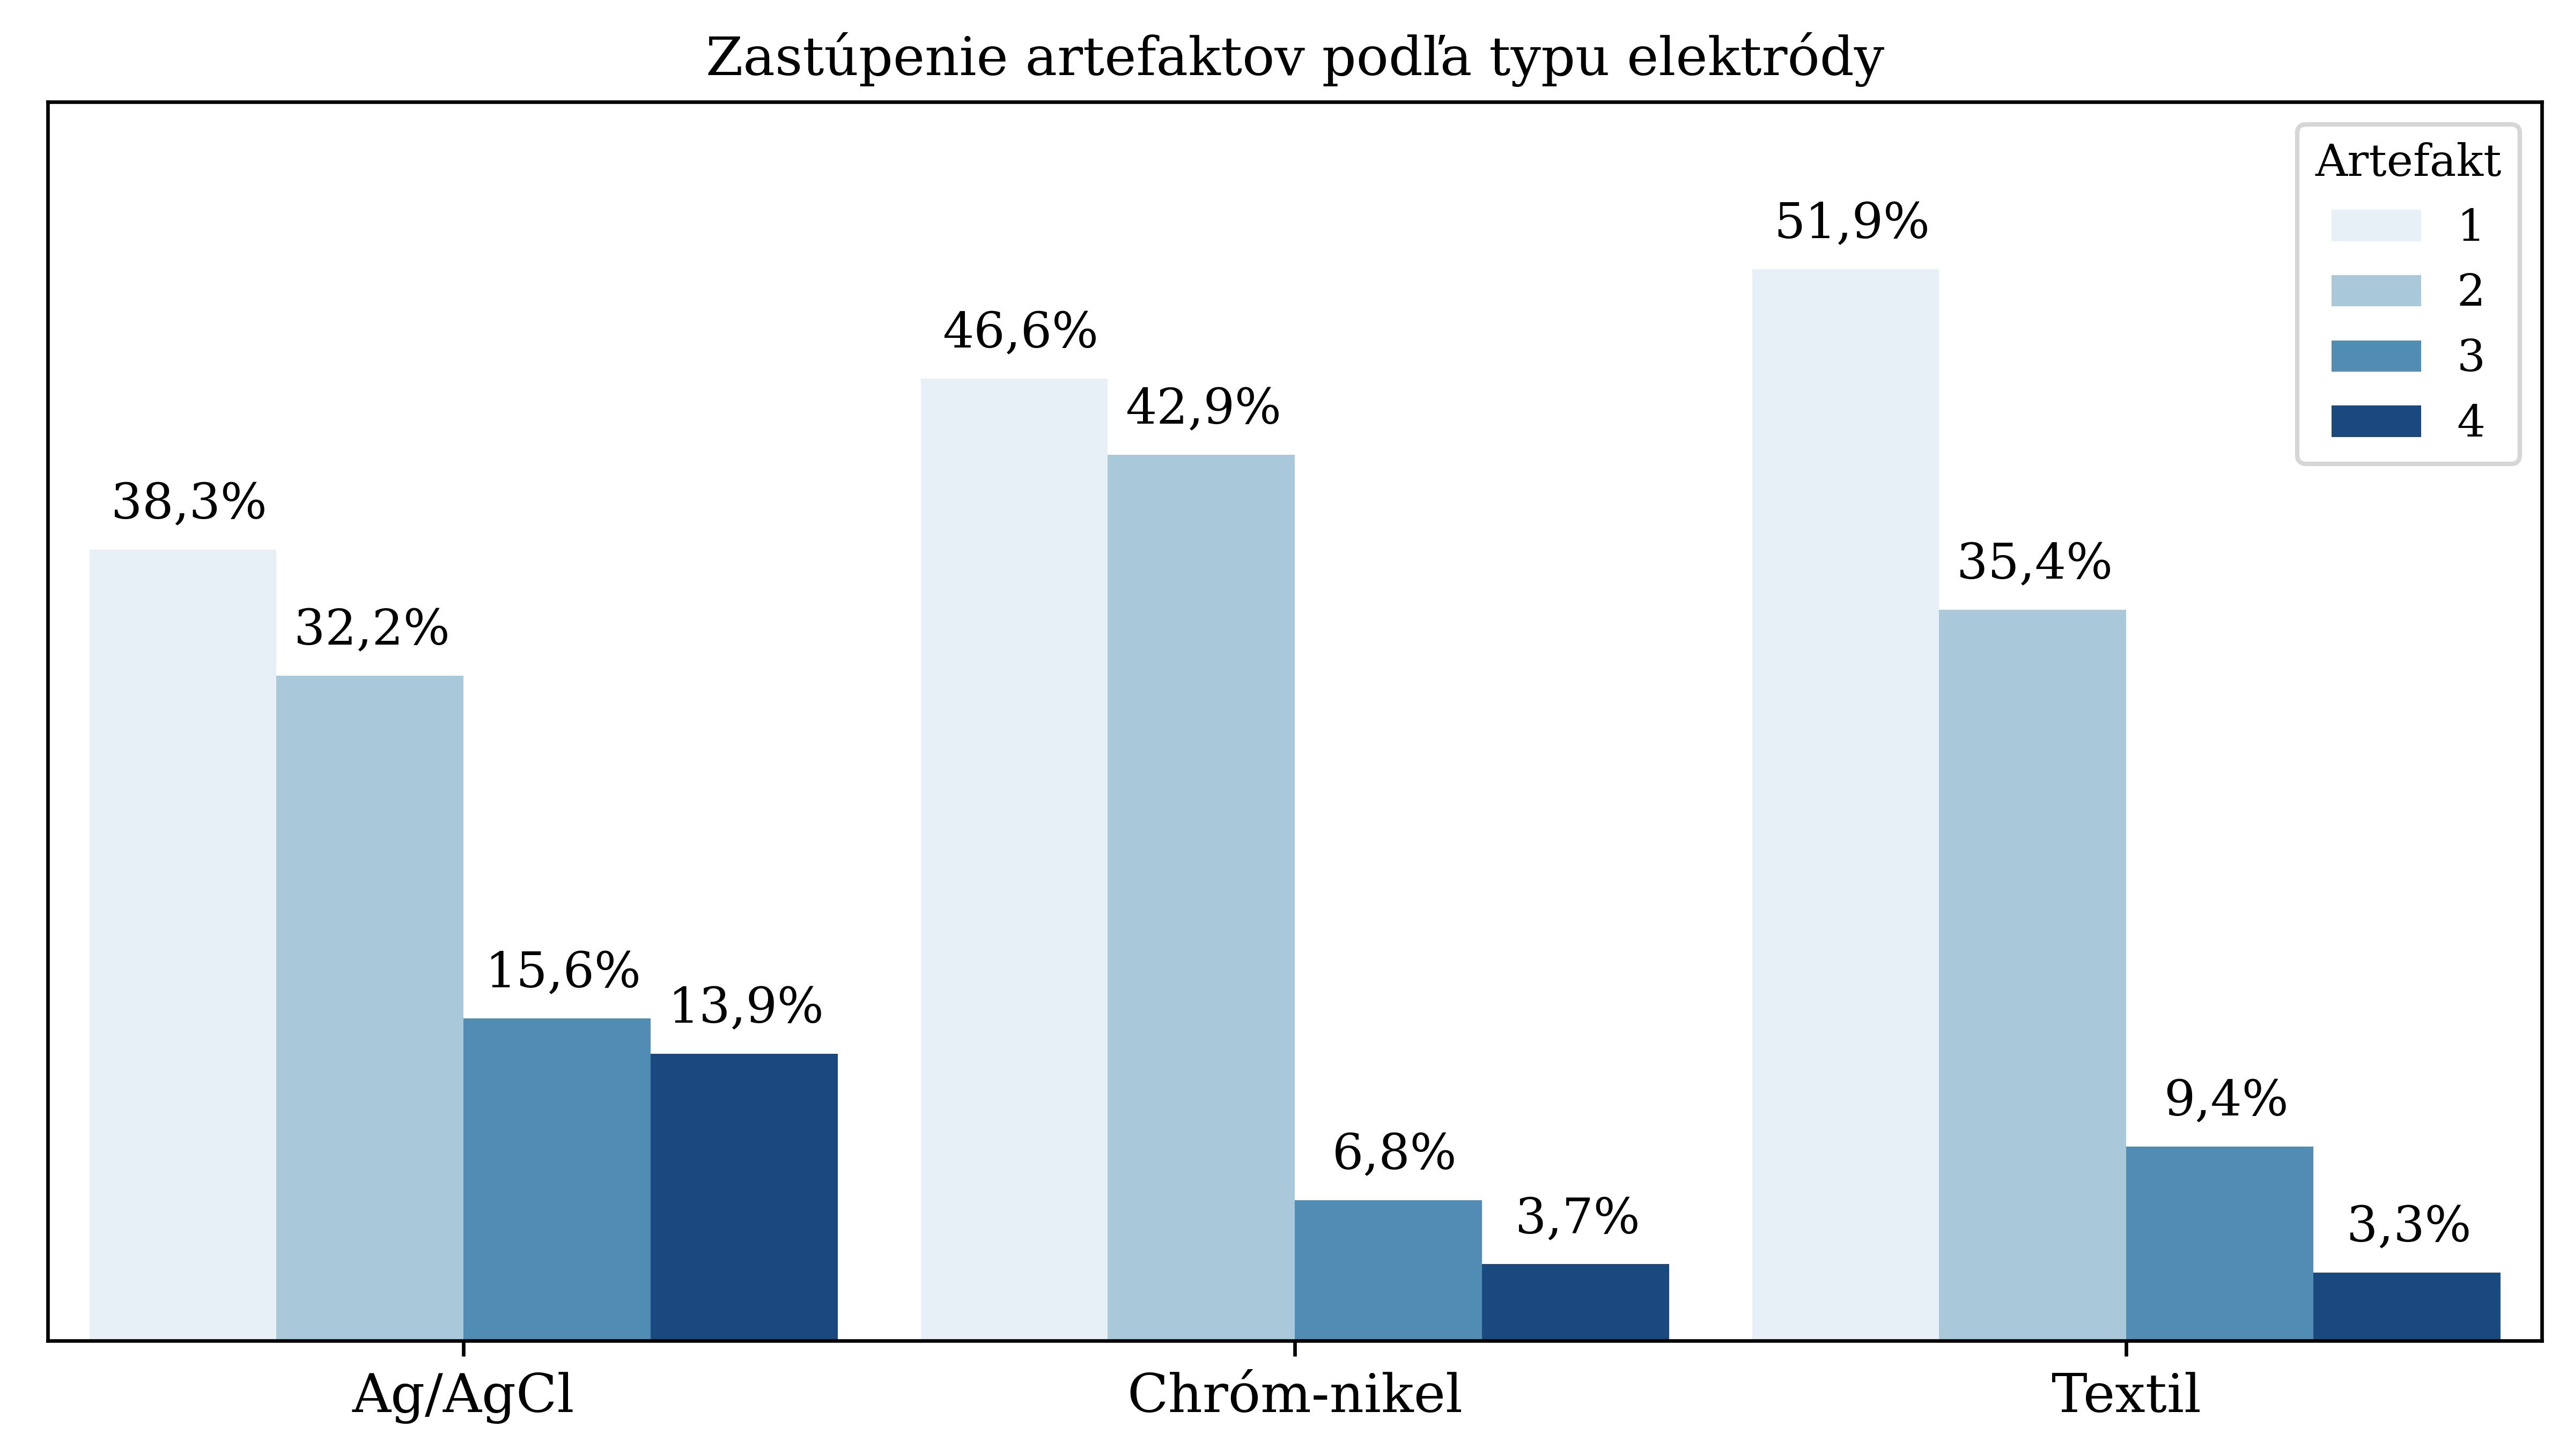
\includegraphics[scale=0.07]{img/electrode_stats_2.jpg}
    \caption{Podiel artefaktov podľa typu typu elektródy.}
    \label{fig:electrode_stats_2}
\end{figure}


%---------------------------------------------------------------
\section{Klasifikácia pohybových aktivít}
%---------------------------------------------------------------

Po všeobecnom predspracovaní dát, popísanom v predošlej kapitole, spočívala príprava dát na~trénovanie modelu v rozdelení dátovej sady na trénovaciu, testovaciu a validačnú množinu, pričom dáta boli rozdelené v pomere 80 \% -  20 \% - 10 \%. Trénovacia množina bola použitá na trénovanie modelu, validačná na ladenie hyperparametrov a sledovanie priebehu trénovania. Testovacia množina bola použitá striktne iba na finálne vyhodnotenie. Dáta boli rozdelené pomocou stratifikovaného výberu, aby rozdelenie vo všetkých troch množinách zodpovedalo pomeru výstupnej triedy v dátach.

%---------------------------------------------------------------
\subsection{Model}
%---------------------------------------------------------------

Architektúru výsledného modelu je možné vidieť na obrázku \ref{fig:activity_classification_model}, ide o hlboký konvolučný model s nasledovnými vstupmi a výstupmi:
\begin{itemize}
    \item \textbf{Vstupy:} Časová a frekvenčná zložka EKG signálu.
    \item \textbf{Výstupy:} Vektor pravdepodobností príslušnosti k jednotlivým triedam, rozmer ktorého je~definovaný počtom pohybových aktivít.
\end{itemize}

Kvôli klasifikácii do viacerých tried je na výstupnej vrstve použitá aktivačná funkcia \textit{softmax} \ref{eq:3}, takže výstupné neuróny obsahujú pravdepodobnosti príslušnosti k jednotlivým triedam. Cieľová premenná musela byť pomocou one-hot kódovania prevedená do rovnakého tvaru, finálne predikcie sú získavané funkciou \textit{argmax}. Ako aktivačná funkcia v skrytých vrstvách bola zvolená \textit{ReLU}, použitie ktorej je štandardom v hlbokých konvolučných architektúrach, lebo je~efektívna na výpočet a dokáže predchádzať miznúcemu gradientu. Model bol trénovaný pomocou optimalizačného algoritmu Adam a ako stratová funkcia pre klasifikáciu do viacerých tried bola zvolená \textit{kategorická krížová entrópia} \ref{eq:4}.

Základnú architektúru sme hľadali empiricky - začali sme jednoduchou architektúrou s~troma plne prepojenými vrstvami, ich počet sme postupne zvyšovali až kým nedošlo k preučeniu modelu a presnosť klasifikácie na validačnej množine prestala rásť. Z hľadiska rozmerov plne prepojených vrstiev sme najlepšie výsledky dosiahli ich postupným zmenšovaním, pričom takýto model vykonáva downsampling operáciu na vstupných dátach.

Následne sme skúmali vplyv jednotlivých vstupov modelu na úspešnosť klasifikácie. Na samom začiatku sme na vstup modelu dávali iba EKG segmenty, teda časovú zložku dát. Pri~najlepšej nájdenej hlbokej architektúre sme dokázali týmto prístupom dosiahnuť presnosť iba 40 \% na validačnej množine. Po modifikácii tej istej architektúry tak, aby na vstup brala aj~frekvenčnú zložku dát, presnosť narástla na 64 \% na validačnej množine. 

Skúšali sme rozličné dĺžky frekvenčného spektra, pričom sme boli z hora obmedzení hodnotou 250, ktorá vyplýva z Nyquist-Shannonovho teorému a vzorkovacej frekvencie 500 Hz. Zistili sme, že dĺžka nad 200 Hz už neprinášala do modelu žiadnu užitočnú informáciu. Taktiež odstránenie jednosmernej zložky z EKG signálu nemalo vplyv na kvalitu klasifikácie. Posledný prístup, ktorý sme z hľadiska vstupov skúmali, bolo pridanie informácie o použitom type elektródy, tá však tiež neprinášala modelu žiadnu užitočnú informáciu.

Následným pridaním jedno-dimenzionálnych konvolučných vrstiev na spracovanie frekvenčnej zložky úspešnosť klasifikácie narástla na 77 \%. Z hľadiska konvolučných vrstiev sme skúšali rozličné počty od 1 až po 5, počty filtrov od 16 po 256, najlepšie výsledky sme dosiahli pre dve po sebe idúce vrstvy s 64 a 128 filtrami, a následnými max poolingovými vrstvami.

\begin{figure}[H]
    \centering    
    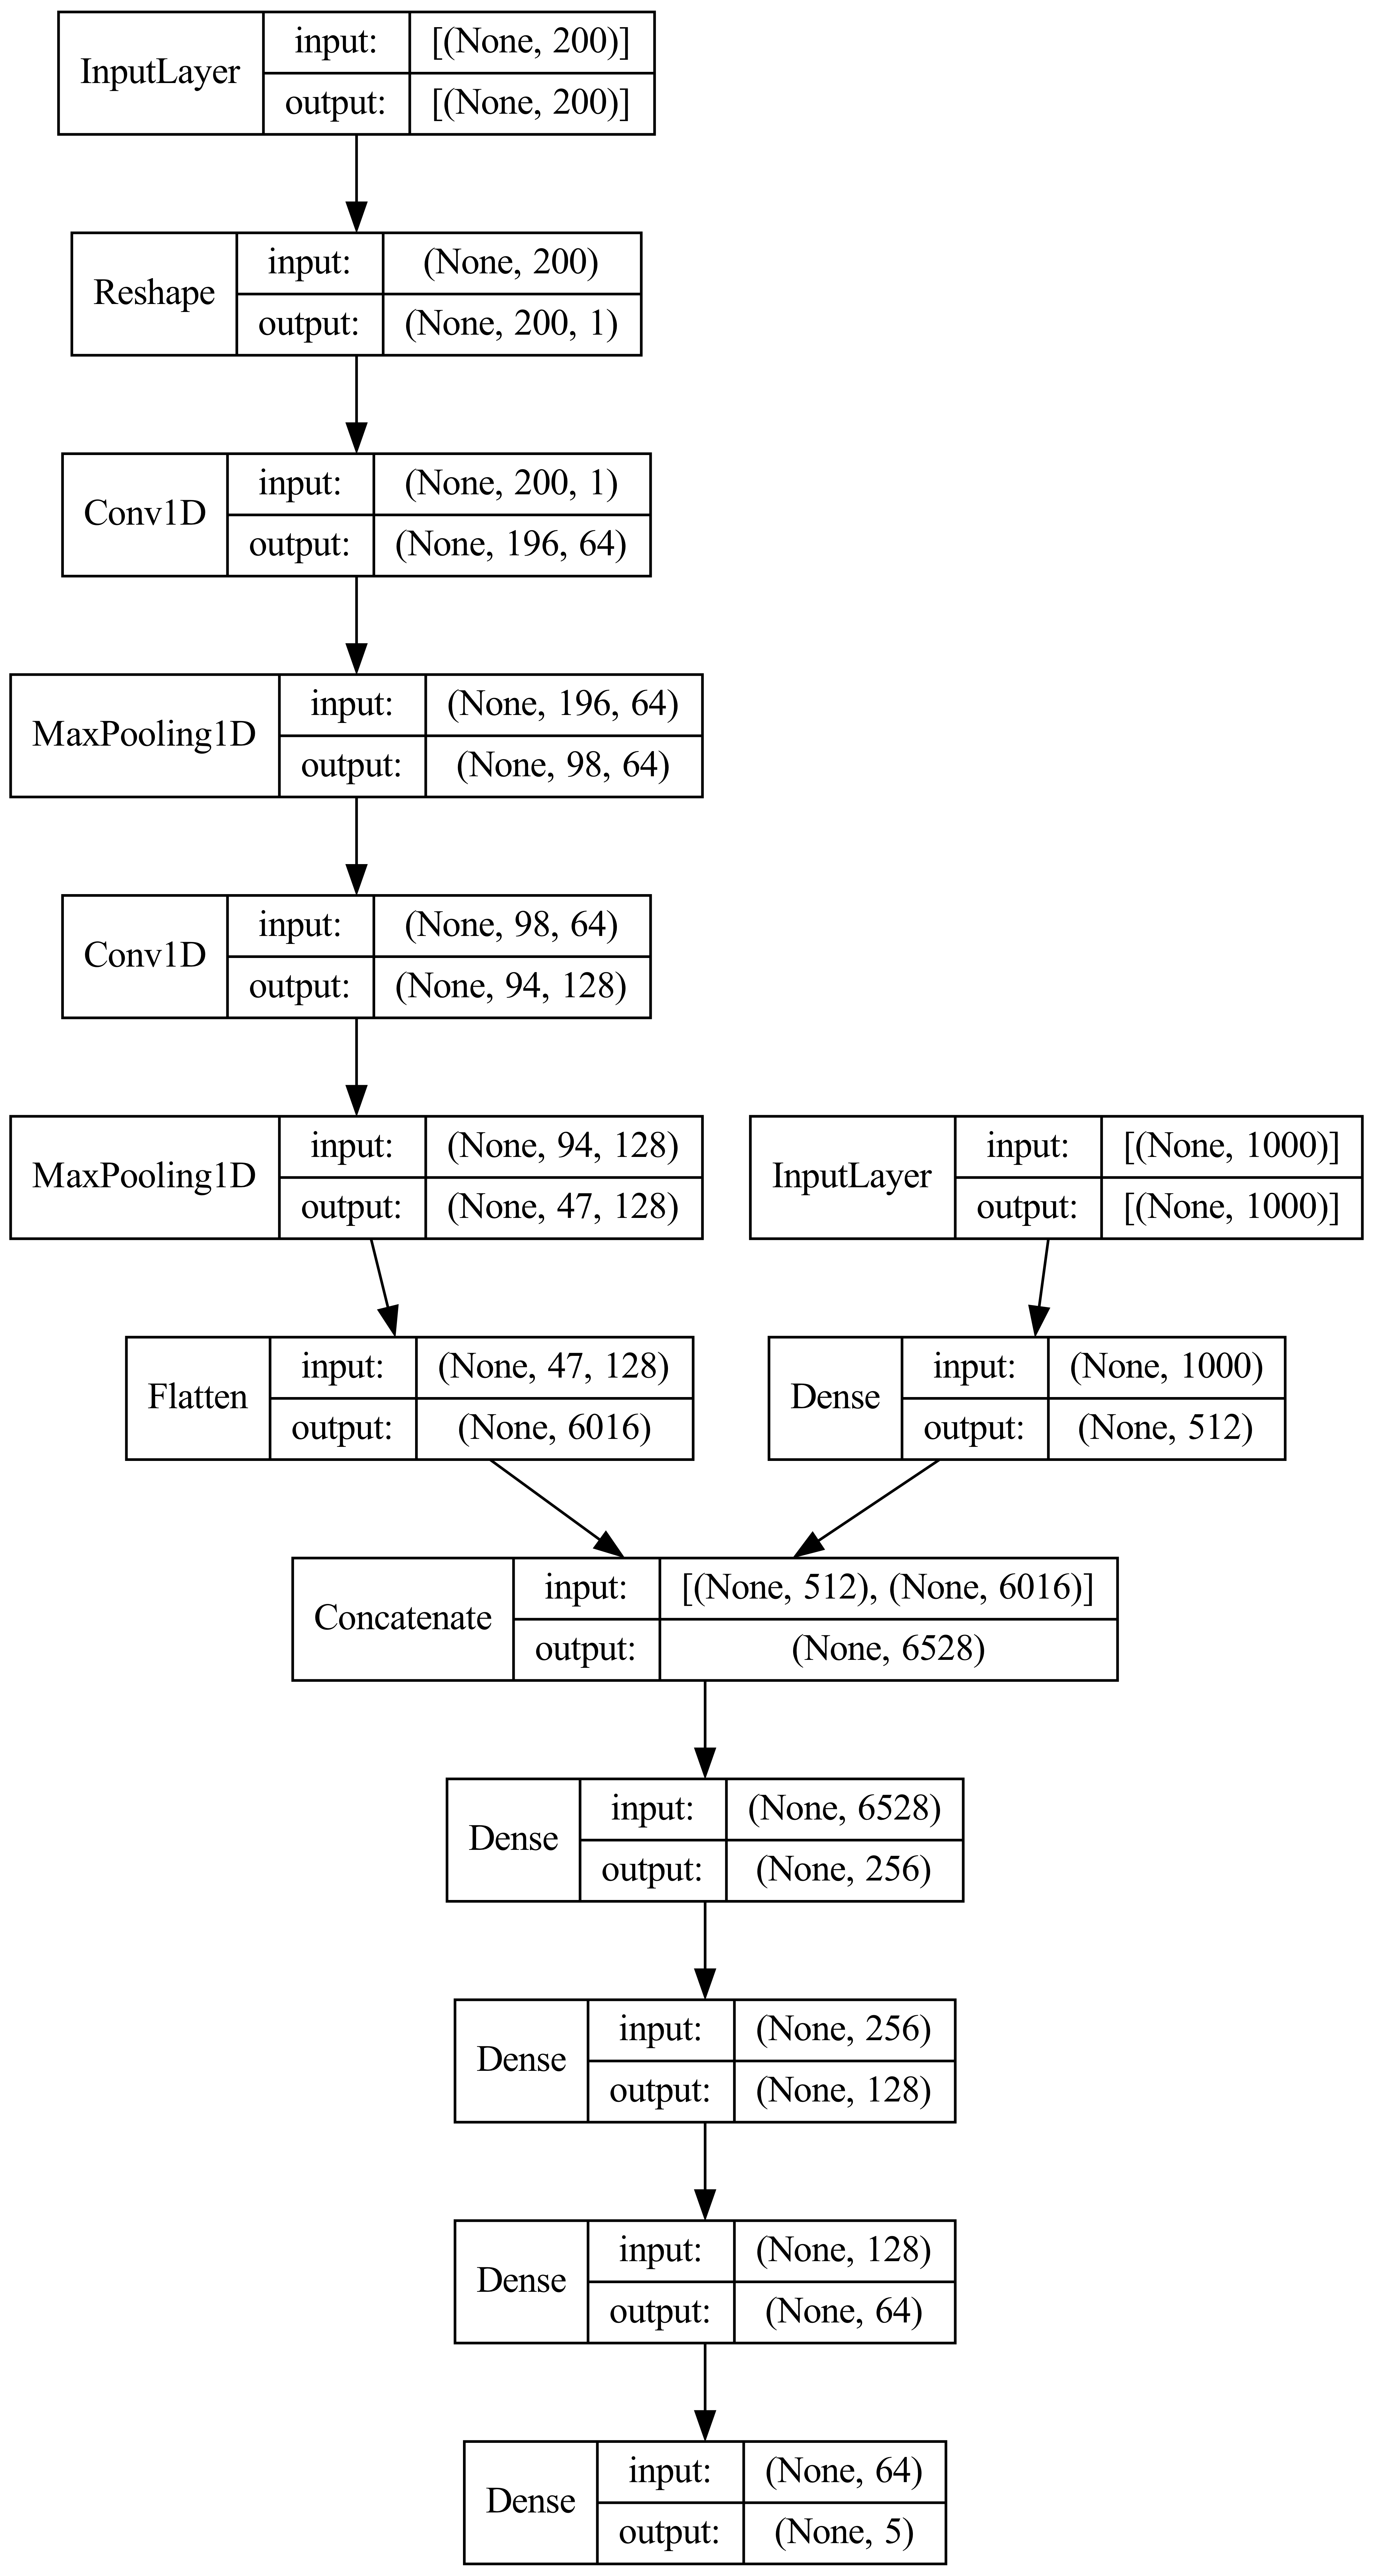
\includegraphics[scale=0.075]{img/activity_classification_model.png}
    \caption{Výsledný model pre klasifikáciu pohybových aktivít.}
    \label{fig:activity_classification_model}
\end{figure}

V priebehu experimentov boli pomocou metódy každý s každým ladené nasledovné hyperparametre a ich hodnoty, \textbf{najlepšia nájdená kombinácia je zvýraznená}. Keďže táto metóda je výpočtovo náročná, hľadali sme iba v okolí odpozorovaných hodnôt s dobrými výsledka-mi v experimente.

\begin{tabbing}
    \indent \textbf{batch size} \quad\quad\quad\quad \= - 8, \textbf{16}\\
    \indent \textbf{learning rate}                   \> - 0.005, 0.001, \textbf{0.0005}, 0.0001\\
    \indent \textbf{dropout}                         \> - \textbf{0.0}, 0.1, 0.2, 0.3, 0.4, 0.5\\
    \indent \textbf{weight decay}                    \> - \textbf{0.0}, 0.001, 0.0001\\
    \indent \textbf{kernel size}                     \> - 3, \textbf{5}, 9\\
    \indent \textbf{pool size}                       \> - \textbf{2}, 3\\
\end{tabbing}

Model bol trénovaný po dobu 15 epoch, z grafov vývoju metrík straty a presnosti bolo viditeľné, že dlhšie trénovanie neprináša ďalšiu informáciu. Zároveň ale validačná strata a presnosť modelu nezačali divergovať, takže skoré zastavenie nebolo potrebné. Po nájdení finálnej architektúry a vyladení hyperparametrov sme ešte skúšali natrénovať niekoľko modelov na náhodných podmnožinách dát a predikcie spriemerovať - prístup známy ako ensemble metóda \textit{bagging}. Skúšali sme trénovať 5 až 10 modelov na podmnožinách veľkých 50 \% - 80 \%, výsledky klasifikácie to však nezlepšilo. Na trénovanie výsledného modelu boli použité aj validačné dáta.


%---------------------------------------------------------------
\subsection{Vyhodnotenie klasifikácie}
%---------------------------------------------------------------

\begin{figure}[H]
    \centering    
    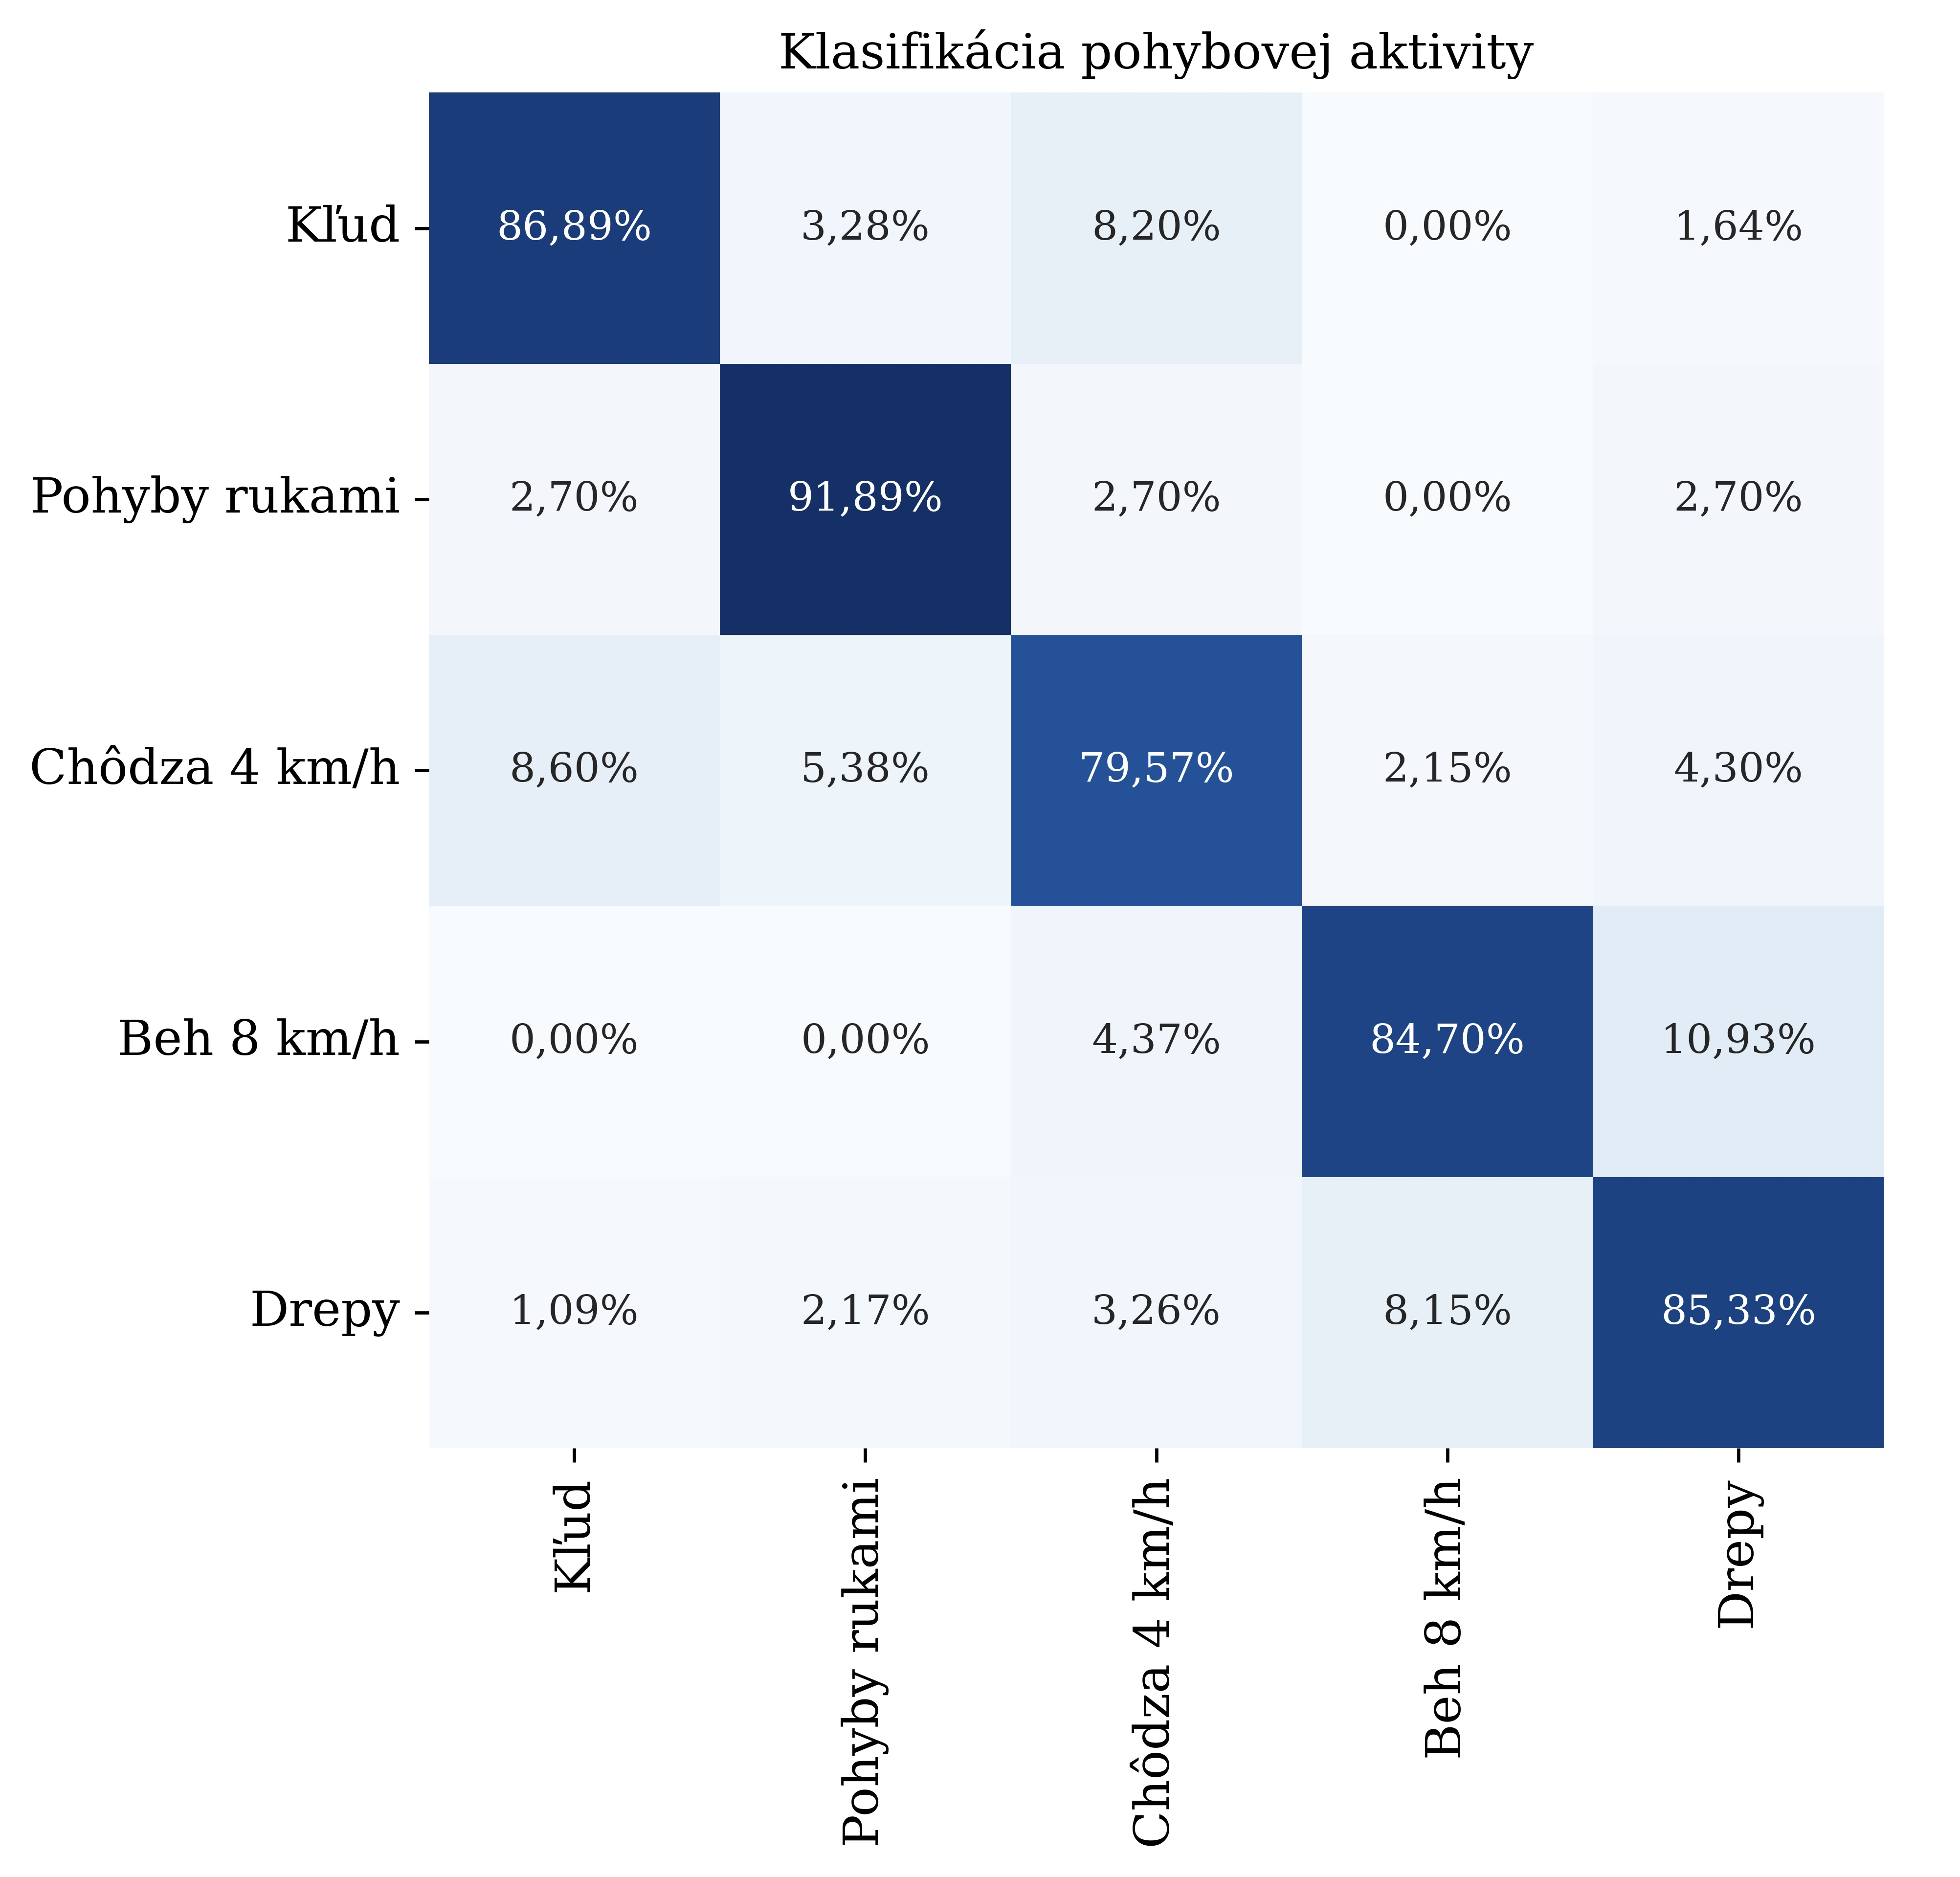
\includegraphics[scale=0.07]{img/confusion_matrix_activity.jpeg}
    \caption{Matica zámen pre klasifikáciu pohybových aktivít.}
    \label{fig:activity_classification}
\end{figure}

Na obrázku \ref{fig:activity_classification} môžeme vidieť výslednú maticu zámen pre klasifikáciu pohybových aktivít do~jednotlivých tried. Celková presnosť, ktorú sme na testovacej množine dosiahli, je \textbf{85,67~\%}. Táto~hodnota je relatívne vysoká vzhľadom na variabilitu EKG záznamov v rámci jednej triedy, keďže boli zaznamenané troma rôznymi elektródami s rozličnými vlastnosťami. Z tabuľky \ref{tab:electrode_stats} uvedenej pri vyhodnotení elektród je vidieť, že pre každú aktivitu, okrem kľudu, obsahujú záznamy rozličné úrovne rušenia. Napriek tomu si s touto variabilitou model do veľkej miery dokázal poradiť.


%---------------------------------------------------------------
\section{Klasifikácia pohybových artefaktov}
%---------------------------------------------------------------

Keďže vstupné dáta pre oba problémy sú rovnaké a výstupy sa líšia iba v počte tried, predpokladali sme, že výsledné architektúry jednotlivých modelov by mohli byť podobné. Navrhovať architektúru modelu sme začali na probléme klasifikácie aktivít, keďže ten má presne zadefinované triedy, a následne sme sa pri klasifikácii pohybových artefaktov odrazili od vzniknutého modelu. Dáta boli rovnako ako pri klasifikácii pohybových aktivít rozdelené na trénovaciu, testovaciu a validačnú množinu v pomere 80 \% -  20 \% - 10 \%. Jediným rozdielom bolo, že množiny sme delili pomocou stratifikovaného výberu vzhľadom k triede pohybových artefaktov.

Kvôli zisteniu, že dátová sada je nevyvážená z hľadiska pohybových artefaktov, sme vytvorili pomocou náhodného prevzorkovania vyváženú dátovú sadu, vzhľadom k najpočetnejšej triede. Prevzorkovanie sme vykonávali až po rozdelení dát na trénovaciu a testovaciu množinu, aby sme sa vyhli duplikovaniu segmentov z trénovacích dát do testovacích. Sofistikovanejšie techniky prevzorkovania dátovej sady, ako napríklad SMOTE, neprichádzali do úvahy, lebo do dátovej sady zavádzajú šum, ktorý pri pohybových artefaktoch nesie dôležitú informáciu.

%---------------------------------------------------------------
\subsection{Model}
%---------------------------------------------------------------

Architektúra výsledného modelu je takmer rovnaká ako \ref{fig:activity_classification_model}, líši sa až v časti po spojení časového a~frekvenčného vstupu, na obrázku \ref{fig:artefact_classification_model} je preto uvedená architektúra až od tohto bodu. Rozdielom je využitie \textit{dropout} vrstiev, vstupy a výstupy sú nasledovné:
\begin{itemize}
    \item \textbf{Vstupy:} Časová a frekvenčná zložka EKG signálu.
    \item \textbf{Výstupy:} Vektor pravdepodobností príslušnosti k jednotlivým triedam, rozmer ktorého je~definovaný počtom tried pohybových artefaktov.
\end{itemize}

Na výstupnej vrstve je opäť použitá aktivačná funkcia \textit{softmax} \ref{eq:3}, a cieľová premenná musela byť pomocou one-hot kódovania prevedená do rovnakého tvaru. Aktivačná funkcia \textit{ReLU} v skrytých vrstvých, optimalizačný algoritmus Adam a stratová funkcia \textit{kategorická krížová entrópia} \ref{eq:4} zostali oproti predošlému modelu nezmenené.

Rovnako ako pri modeli na klasifikáciu pohybových aktivít sme z hľadiska vstupov skúšali zvýšiť dĺžku frekvenčného spektra, odstrániť jednosmernú zložku, a skúsiť pridať na~vstup typ použitých elektród, opäť nič neprinieslo modelu užitočnú informáciu. Skúšali sne model trénovať aj na vyváženej dátovej sade vygenerovanej pomocou náhodného prevzorkovania, tento prístup však nemal žiaden vplyv na predikciu minoritných tried 3 a 4.

Z hľadiska architektúry pridávanie plne prepojených vrstiev nemenilo presnosť predikcií modelu, odoberanie presnosť zhoršovalo, a ani zmeny v konvolučnej časti modelu nezlepšovali predikcie. Skúšali sme aj variantu, kedy sme časovú aj frekvenčnú zložku paralelne spracovávali konvolučnými vrstvami a získané aktivačné mapy nakoniec spojili do plne prepojených vrstiev, takýto prístup však dosahoval horšie výsledky ako súčasná najlepšia nájdená architektúra.

\begin{figure}[H]
    \centering    
    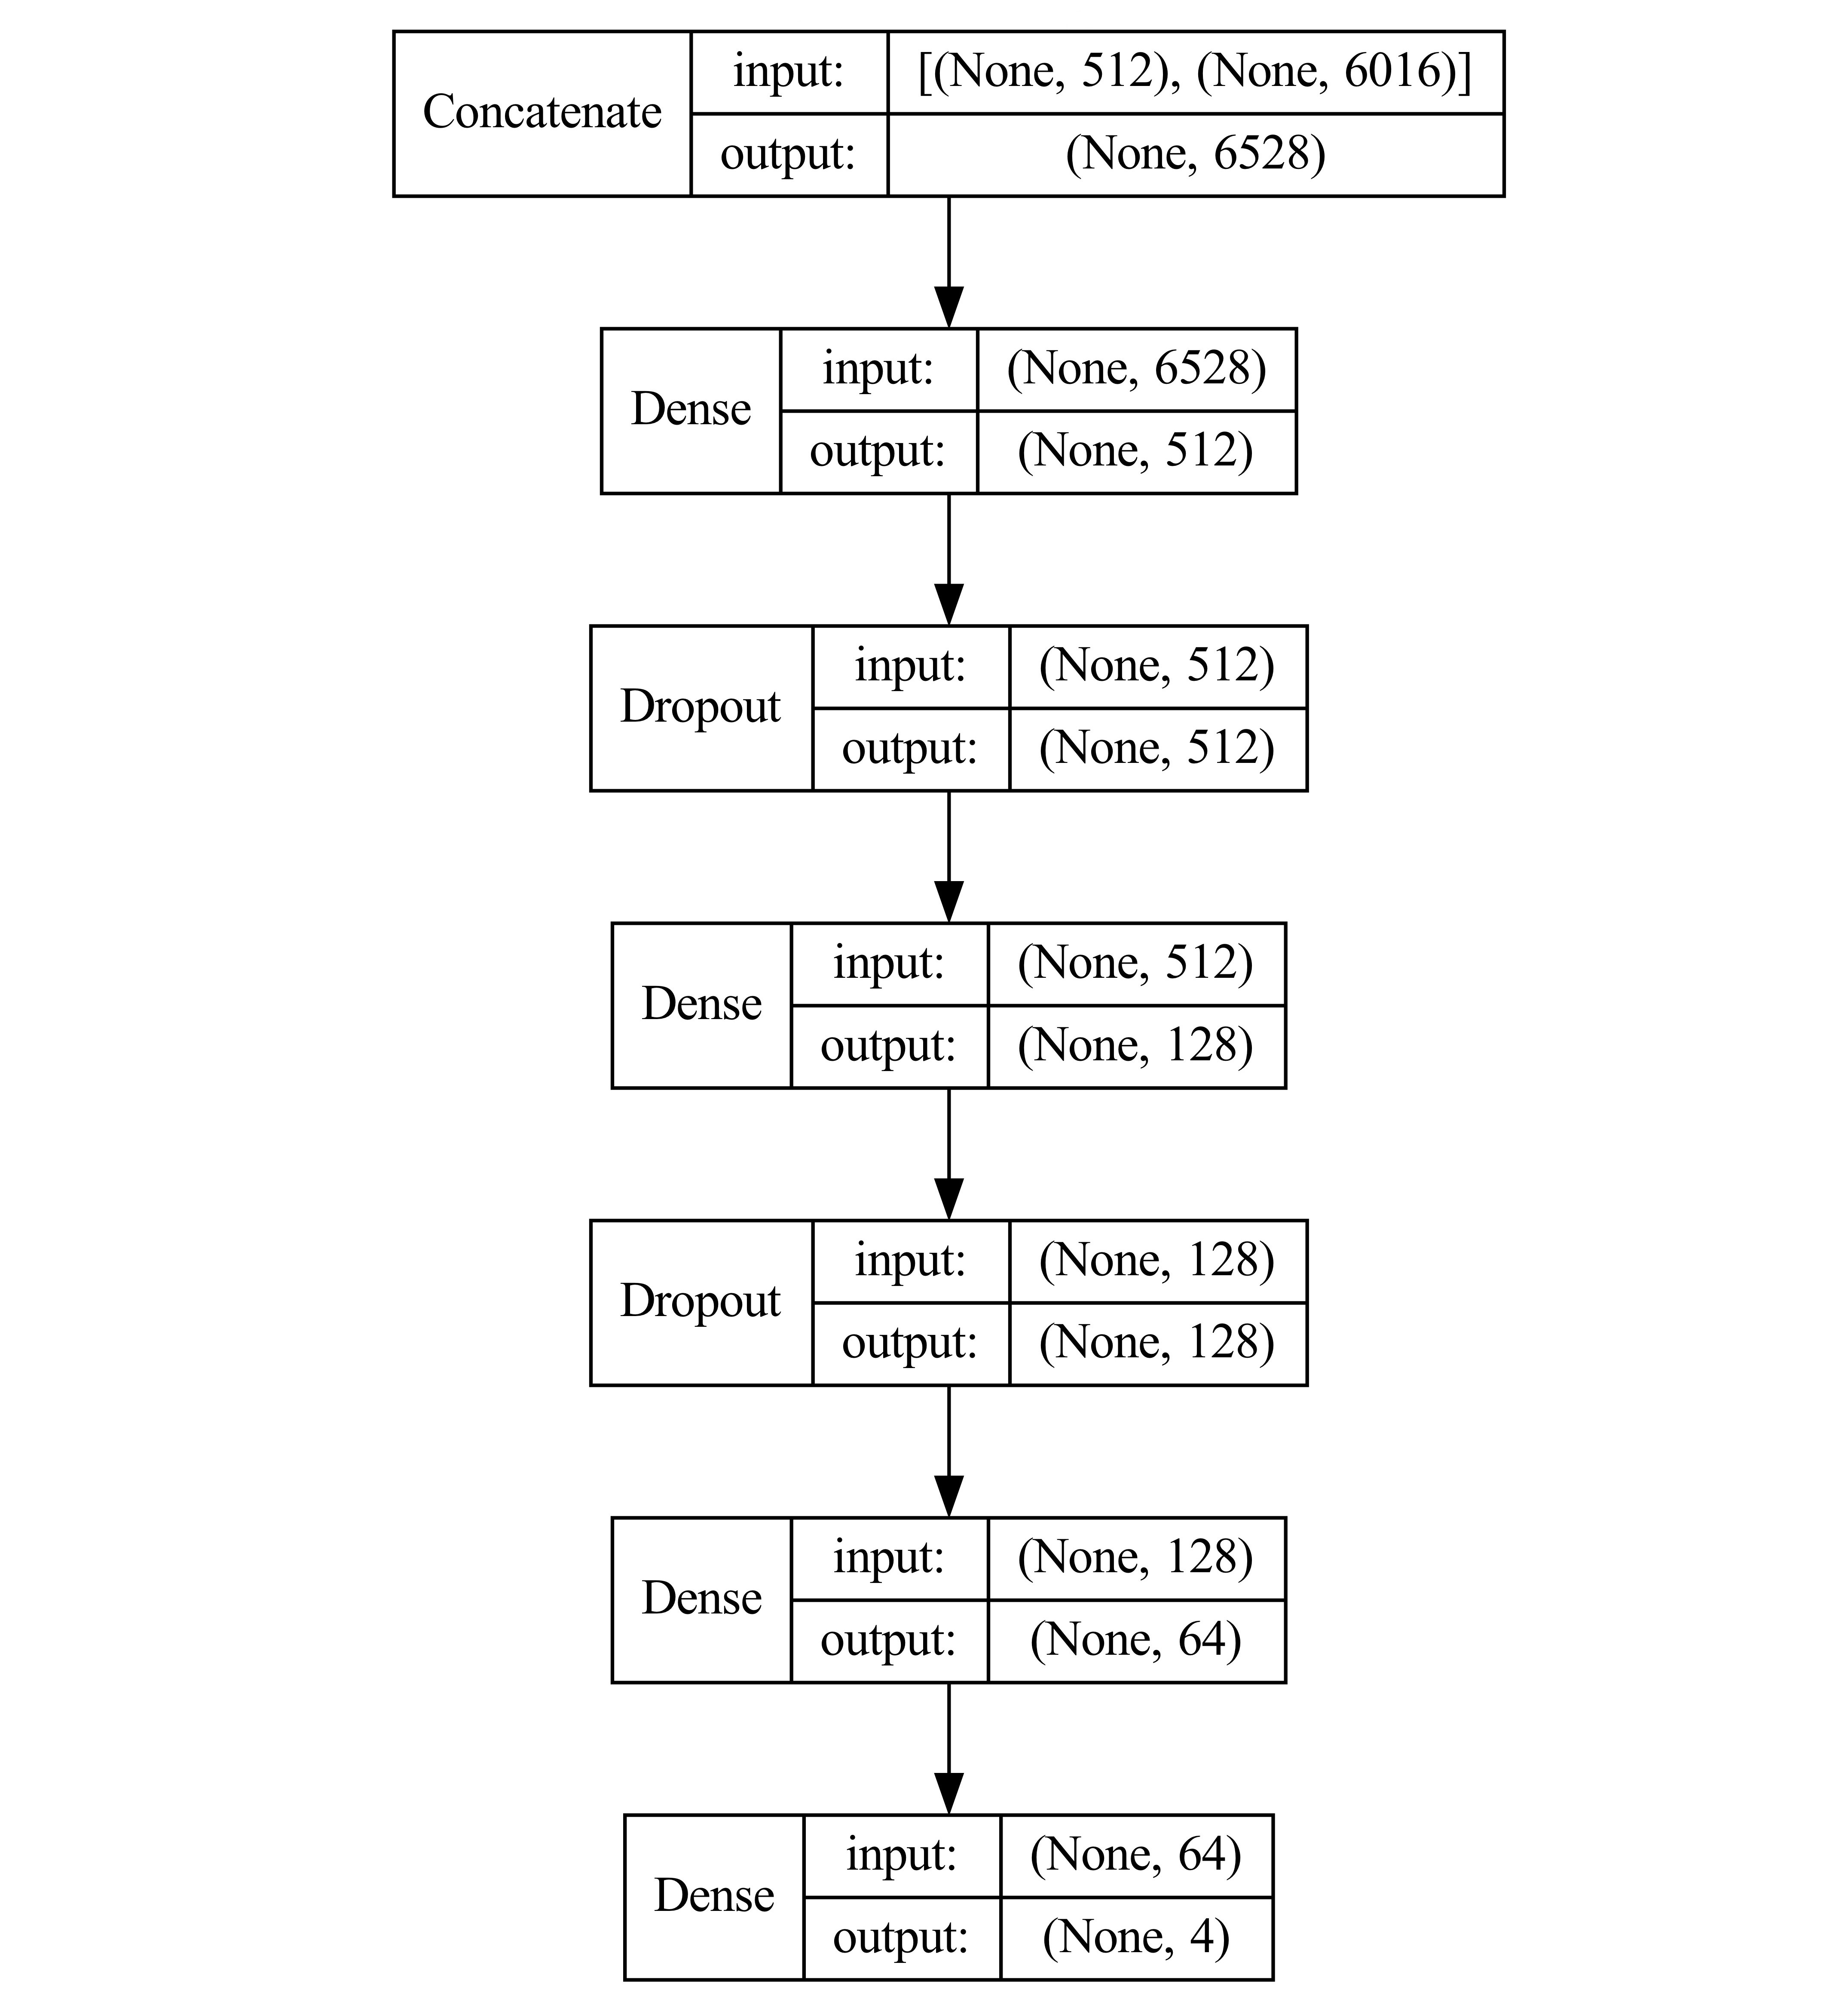
\includegraphics[scale=0.075]{img/artefact_classification_model.jpg}
    \caption{Výsledný model pre klasifikáciu pohybových artefaktov.}
    \label{fig:artefact_classification_model}
\end{figure}

Z grafov vývoja metrík straty a presnosti počas trénovania \ref{fig:metrics_before} je viditeľné, že model je náchylný na preučenie - trénovacia a validačná krivka začali po zopár epochách divergovať. Z metód, ktoré by mohli s týmto problémom pomôcť sme skúšali batch normalizáciu, kedy sme normalizovali výstupy všetkých plne prepojených vrstiev, tá však nepomohla. Zmierniť tento problém sa nám podarilo pridaním \textit{dropout} vrstiev medzi plne prepojené vrstvy, tie náhodne vynulujú niektoré neuróny počas trénovania. Pomohlo aj pridanie slabej L2 regularizácie, ktorá penalizuje kvadráty váh, ako parameter optimalizačného algoritmu Adam.

Hlavné zlepšenie viditeľné na grafoch \ref{fig:metrics_after} sme dosiahli použitím plánovača \textit{learning rate}. Na začiatku definovaná hodnota sa v každej epoche exponenciálne znižuje podľa vzťahu \ref{eq:20}, kde~\textit{k}=0,1 je voliteľný parameter. Okrem výrazného potlačenia divergencie trénovacej a~validačnej straty sa nám podarilo aj stabilizovať priebeh trénovania.

\begin{equation} 
    \label{eq:20}
    lr = lr \cdot e^{(-k) \cdot epoch}
\end{equation}

\begin{figure}[H]    
    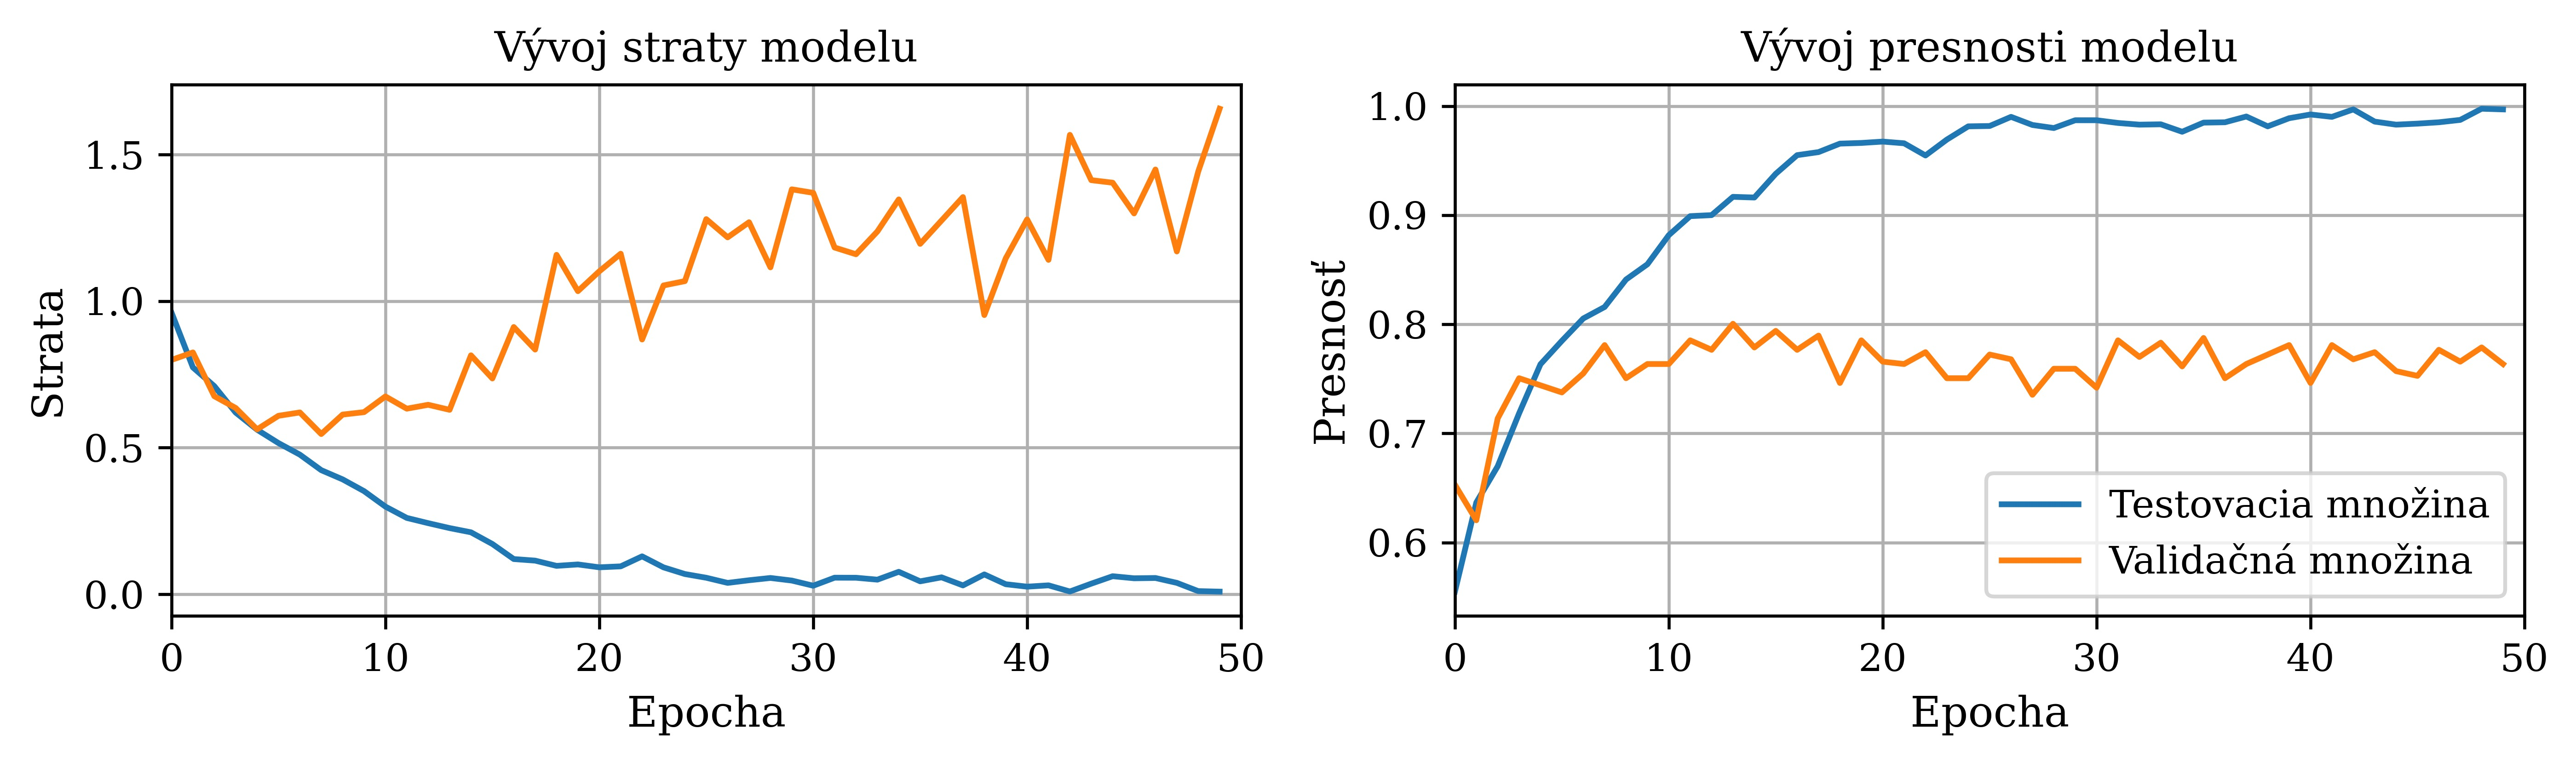
\includegraphics[scale=0.074]{img/metrics_before.jpg}
    \caption{Priebeh vývoju straty a presnosti modelu pred použitím plánovania \textit{learning rate}.}
    \label{fig:metrics_before}
\end{figure}

\begin{figure}[H]    
    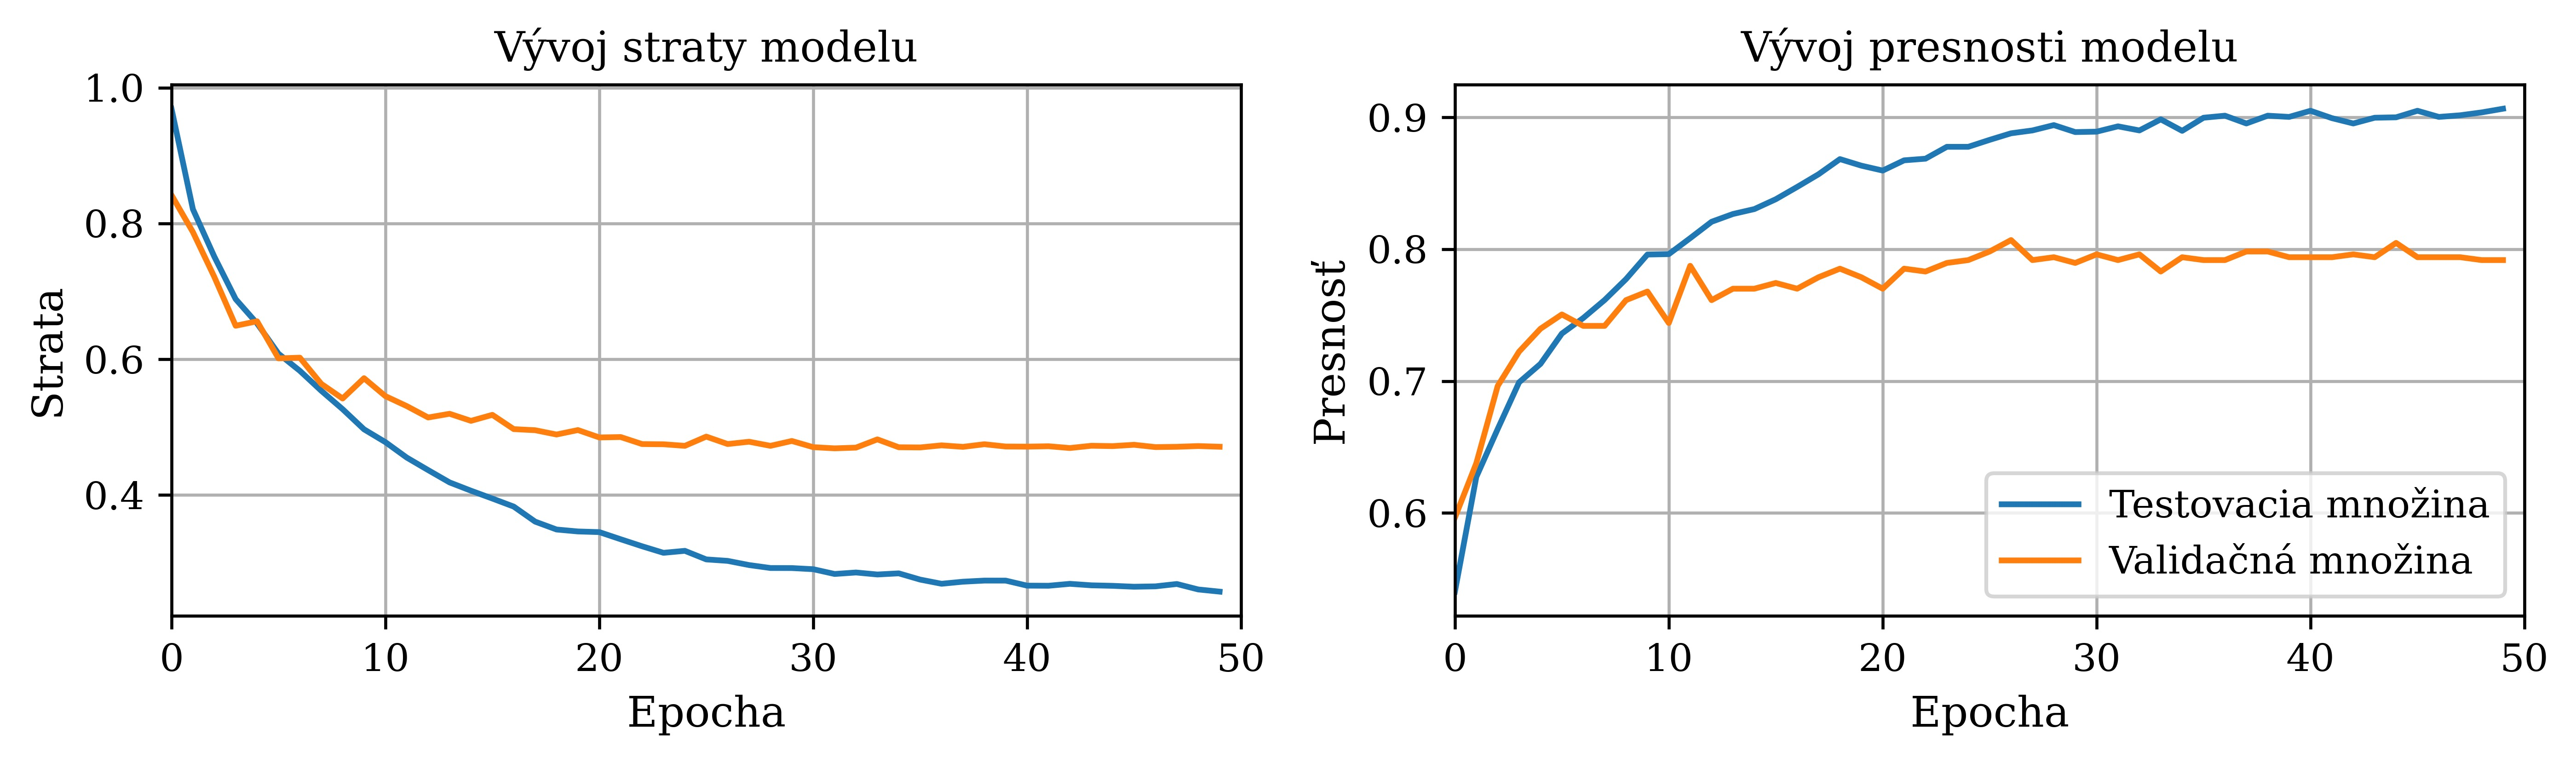
\includegraphics[scale=0.074]{img/metrics_after.jpg}
    \caption{Priebeh vývoju straty a presnosti modelu po použití plánovania \textit{learning rate}.}
    \label{fig:metrics_after}
\end{figure}

Model bol trénovaný po dobu 50 epoch, aj keď z grafov vývoju metrík straty a presnosti počas trénovania bolo viditeľné, že strata aj presnosť modelu sa po zhruba 30 epochách ustálili. Zároveň ale nezačali divergovať, takže skoré zastavenie nebolo potrebné.

V priebehu experimentov boli znovu ladené tie isté hyperparametre a ich hodnoty, \textbf{najlepšia nájdená kombinácia je zvýraznená}.
\begin{tabbing}
    \indent \textbf{batch size} \quad\quad\quad\quad \= - 8, \textbf{16}\\
    \indent \textbf{learning rate}                   \> - 0.005, 0.001, 0.0005, \textbf{0.0001}\\
    \indent \textbf{dropout}                         \> - 0.0, \textbf{0.1}, 0.2, 0.3, 0.4, 0.5\\
    \indent \textbf{weight decay}                    \> - 0.0, 0.001, \textbf{0.0001}\\
    \indent \textbf{kernel size}                     \> - 3, \textbf{5}, 9\\
    \indent \textbf{pool size}                       \> - \textbf{2}, 3\\
\end{tabbing}

Rovnako ako pri modeli na klasifikáciu pohybových aktivít sme skúšali predikovať hodnoty pomocou ensemble metódy \textit{bagging}, pričom jednotlivé modely boli trénované na podmnoži-nách dát veľkých 50 \% - 80 \%, ani v~tomto prípade sme nezaznamenali žiaden nárast presnosti predikcií. Na trénovanie výsledného modelu boli použité aj validačné dáta.

%---------------------------------------------------------------
\subsection{Vyhodnotenie klasifikácie}
%---------------------------------------------------------------

\begin{figure}[H]
    \centering    
    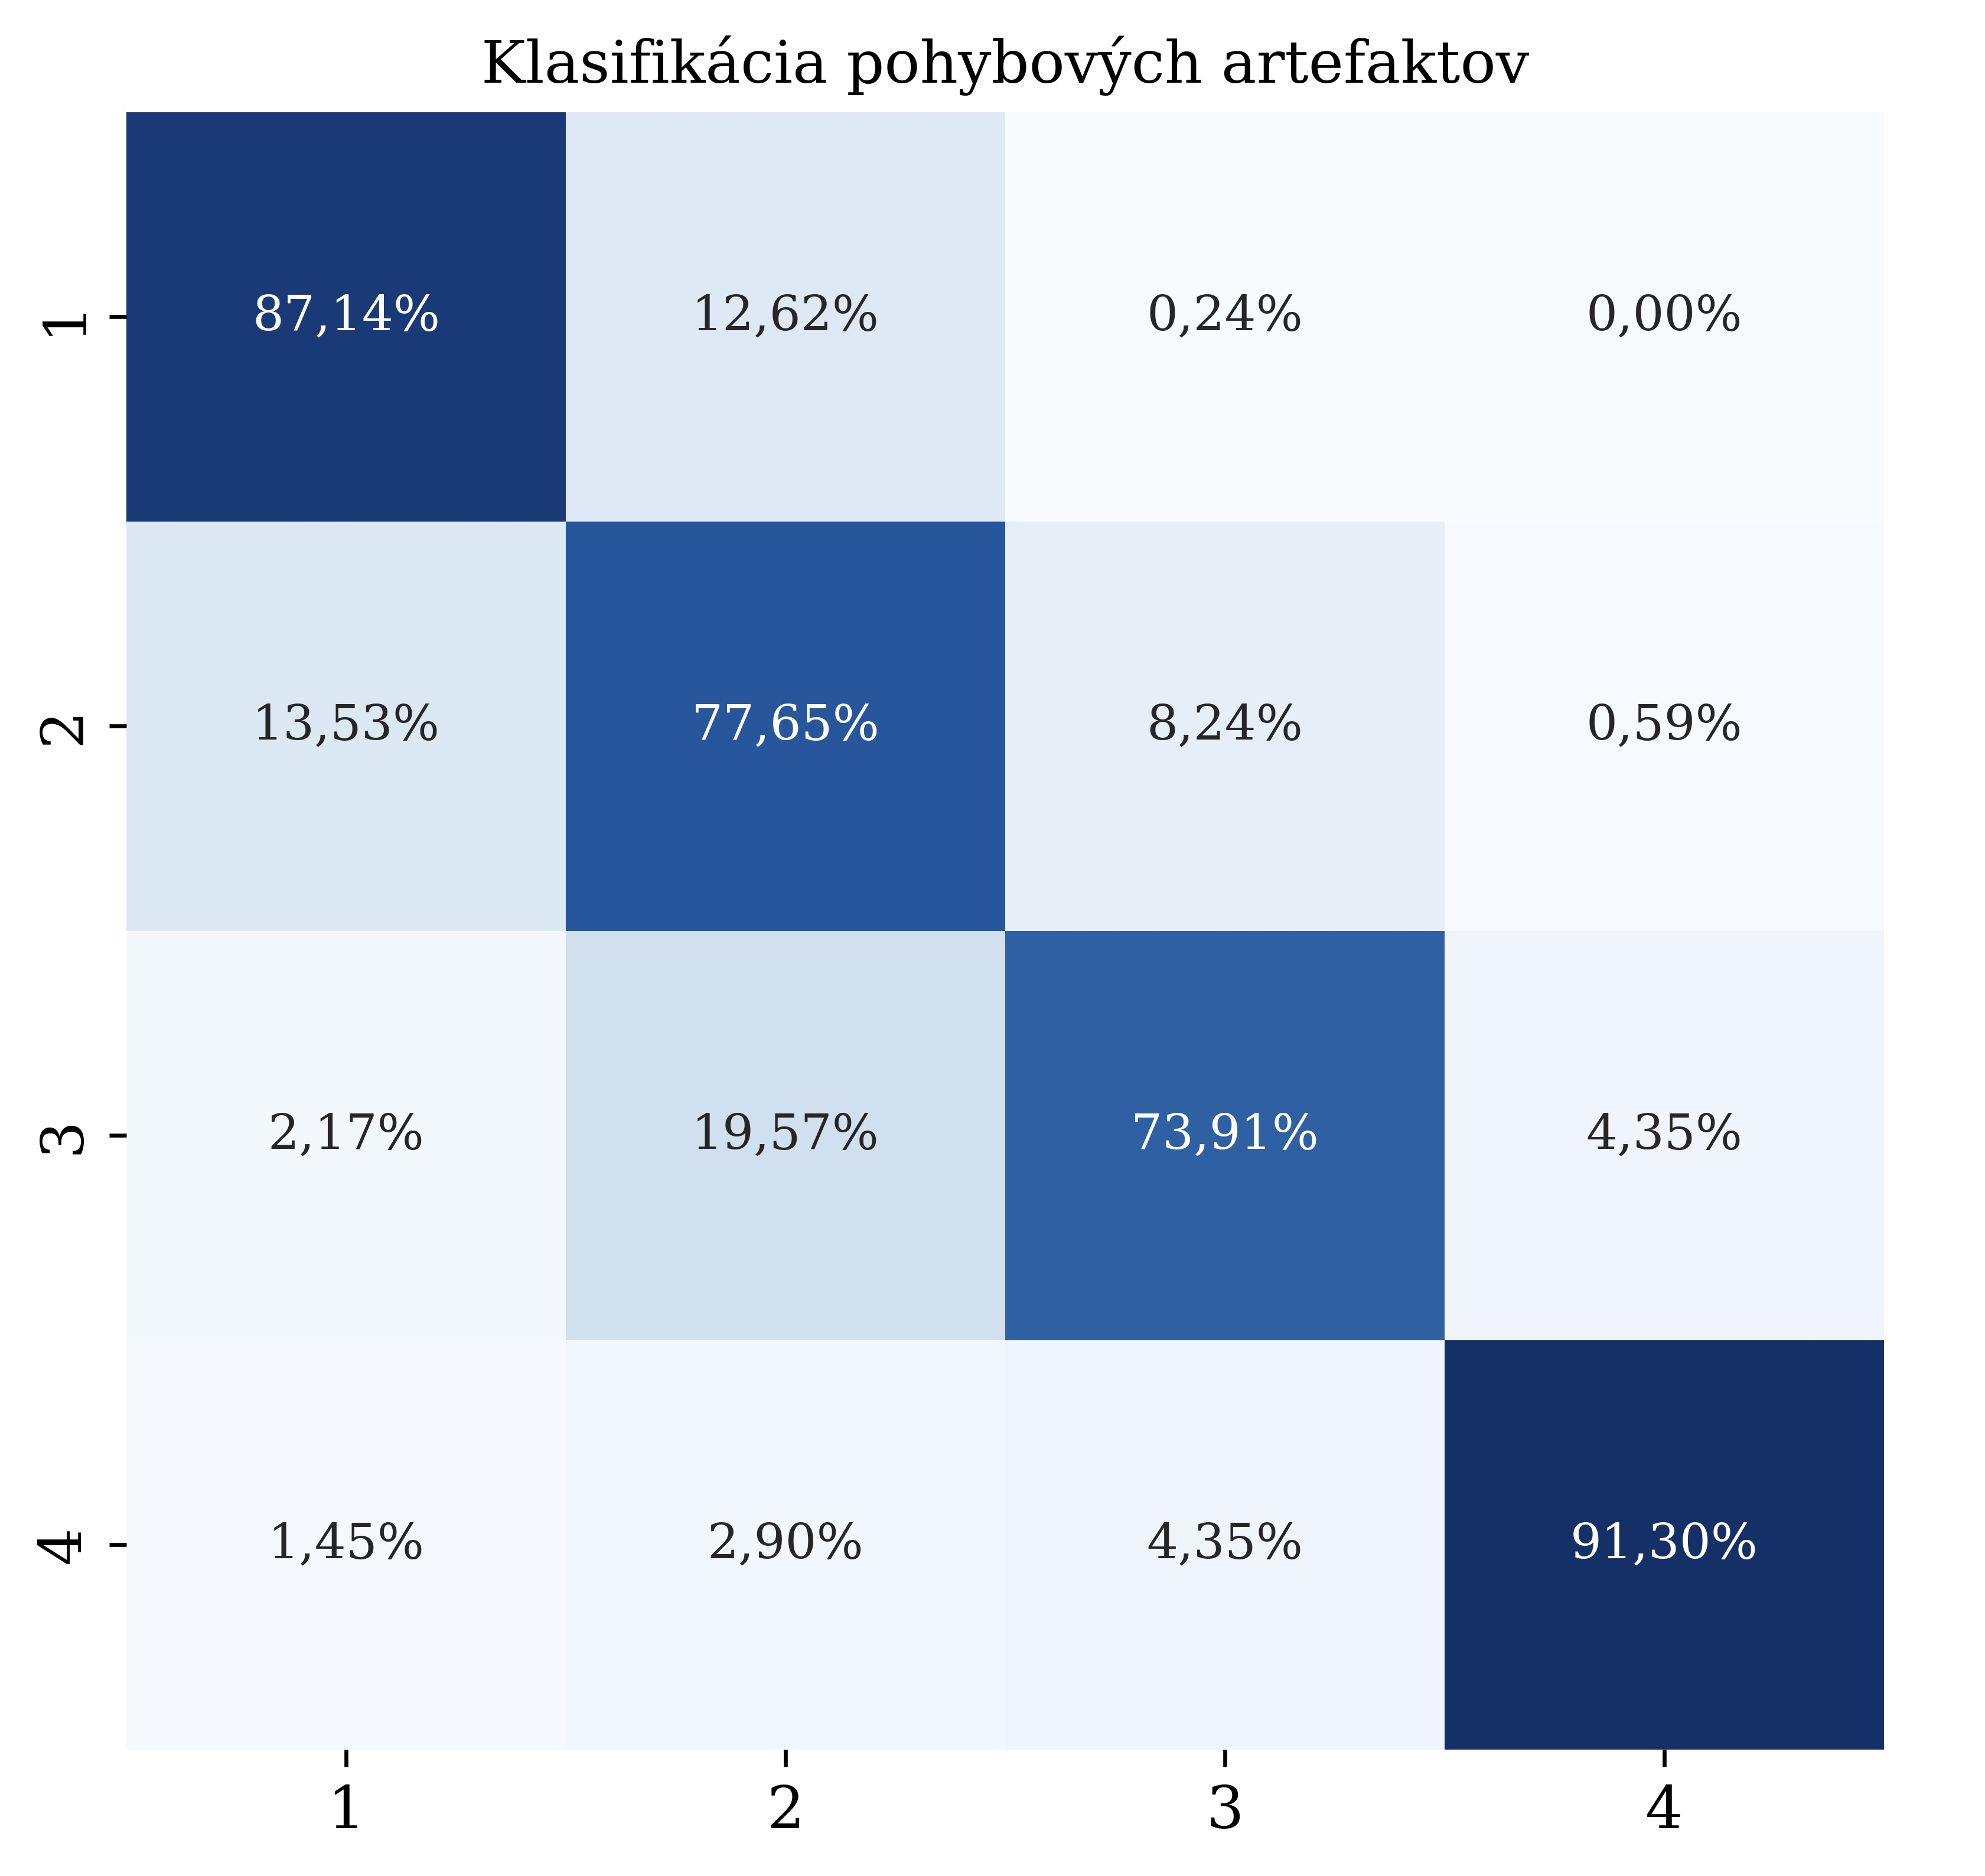
\includegraphics[scale=0.07]{img/confusion_matrix_artefact.jpeg}
    \caption{Matica zámen pre klasifikáciu pohybových artefaktov.}
    \label{fig:artefact_classification}
\end{figure}

Na obrázku \ref{fig:artefact_classification} môžeme vidieť maticu zámen pre klasifikáciu pohybových artefaktov do štyroch tried. Výsledná presnosť na testovacej množine je \textbf{82,63~\%} a hodnota \textit{F1 Score} \textbf{82,68~\%}. To,~že~sú hodnoty týchto dvoch metrík takmer rovné, potvrdzuje vyššie uvedené zistenie, že~použi-tie dátovej sady s vyváženým zastúpením tried neprinieslo modelu žiadnu užitočnú informáciu. Aj keď bol model trénovaný na nevyváženej dátovej sade, naučil sa rovnako dobre predikovať minoritné aj majoritné triedy.

Kým trieda 4 je jasne zadefinovaná nečitateľnosťou srdečného rytmu, rozdiely medzi ostatnými troma triedami sú menej výrazné, čo potvrdzujú aj nasledujúce výsledky. \textit{Precision} a \textit{recall} pre jednotlivé triedy je možné vidieť v tabuľke \ref{tab:artefact_classification}. Z tabuľky je zjavné, že model má~najväčší problém s klasifikáciou tried 2 a 3. Zároveň môžeme v matici zámen vidieť, že model najčastejšie zamieňal predikcie pre triedy 1 a 2 a pre triedy 2 a 3. 

\begin{table}[H]\centering
\caption[\textit{Precision} a \textit{recall} pre klasifikáciu pohybových artefaktov.]{~\textit{Precision} a \textit{recall} pre klasifikáciu pohybových artefaktov.}\label{tab:artefact_classification}
    \begin{tabular}{l|c|c}
    	\textbf{Artefakt} & \textit{\textbf{Precision (\%)}} & \textit{\textbf{Recall (\%)}} \tabularnewline \hline 
     	\textbf{1}        & 88,20	                      &  87,14                           \tabularnewline \hline
     	\textbf{2}	      & 78,34	                      &  77,65                           \tabularnewline \hline
        \textbf{3}	      & 68,00	                      &  73,91                           \tabularnewline \hline
        \textbf{4}	      & 91,30	                      &  91,30                           \tabularnewline
    \end{tabular}
\end{table}


\begin{figure}[H]
    \centering    
    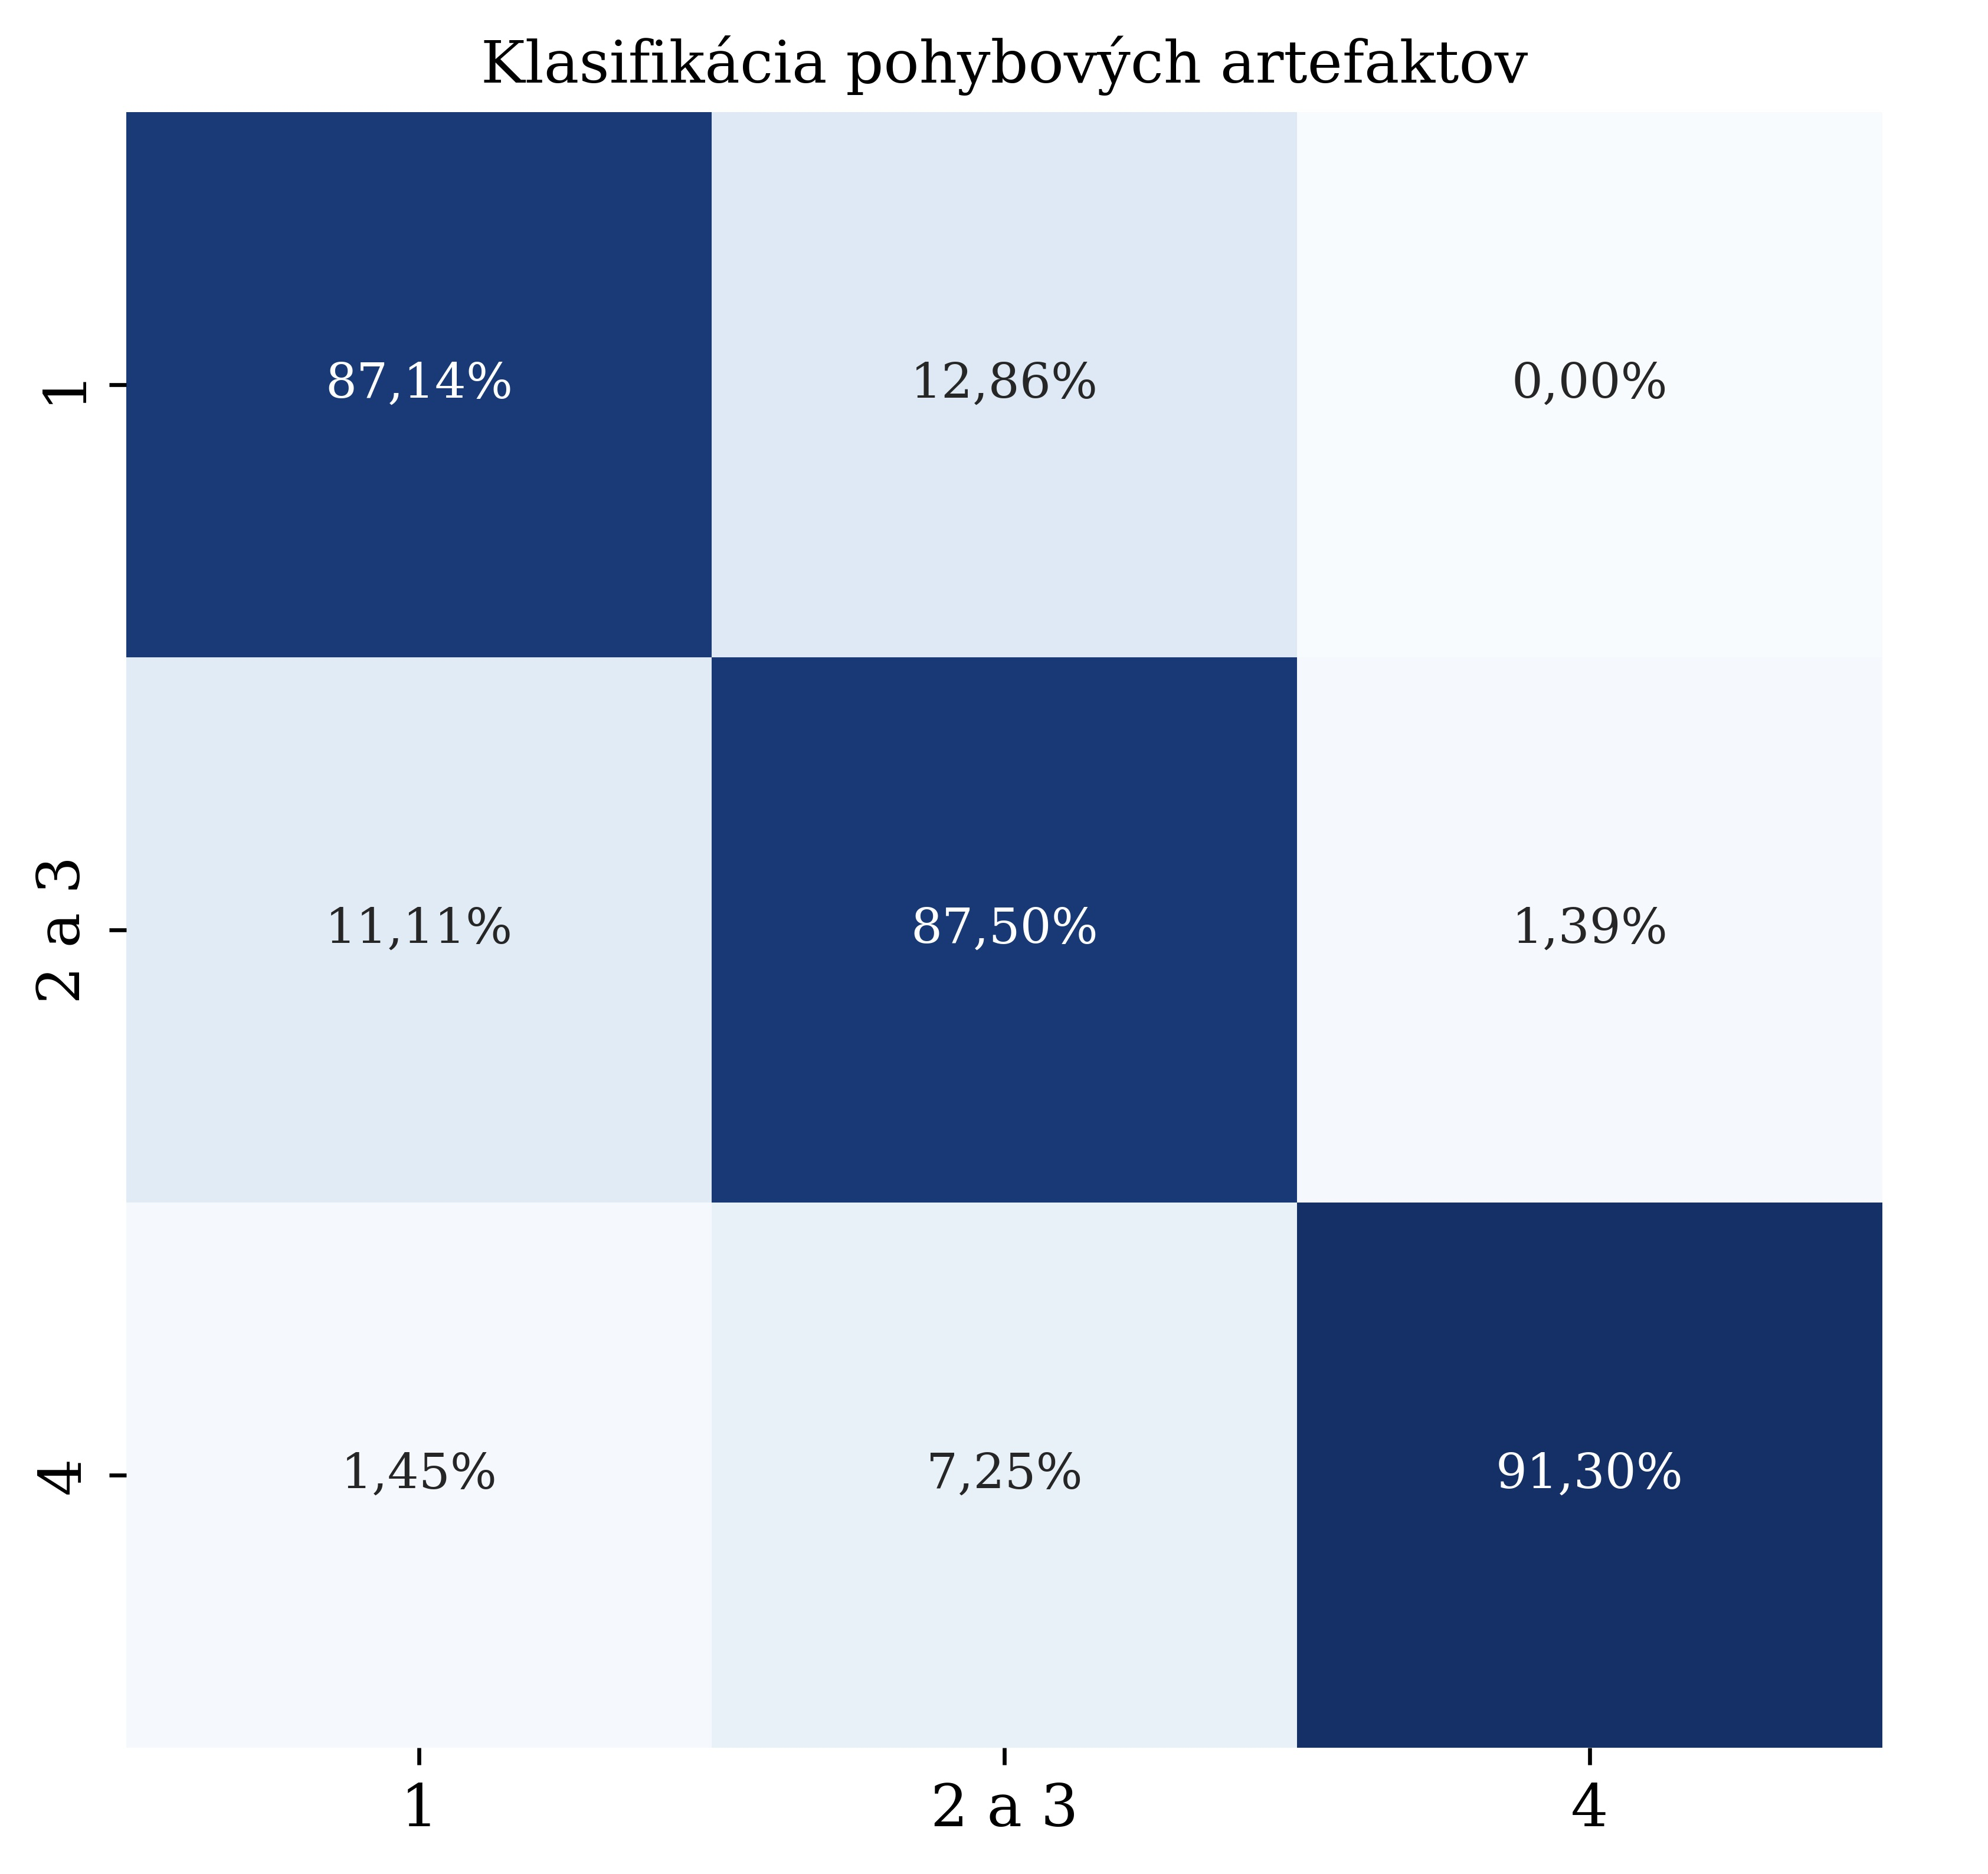
\includegraphics[scale=0.07]{img/confusion_matrix_merged.jpeg}
    \caption{Matica zámen pre klasifikáciu pohybových artefaktov po zlúčení tried 2 a 3.}
    \label{fig:artefact_classification_merged}
\end{figure}

Zlúčením predikcií pre triedy 2 a 3 sa celkové výsledky výrazne zlepšili, ako je vidieť v~matici zámen na obrázku \ref{fig:artefact_classification_merged}. Presnosť aj \textit{F1 score} na testovacej množine narástli na \textbf{87,62~\%}, hodnoty metrík \textit{precision} a \textit{recall} pre jednotlivé triedy je možné vidieť v tabuľke \ref{tab:artefact_classification_merged}. Takéto zlúčenie tried má aj praktický zmysel. V triede 1 sú obsiahnuté segmenty, ktoré sa dajú v praxi využiť na získanie srdečného rytmu aj interpretáciu EKG krivky, trieda 4 obsahuje segmenty, ktoré môžeme úplne odstrániť, lebo z hľadiska interpretácie EKG záznamu neposkytujú žiadnu informáciu. Zlúčená prostredná trieda takto obsahuje segmenty, ktoré sa dajú použiť na detekciu srdečného rytmu, iné charakteristiky z nich už však nemusia byť čitateľné.

\begin{table}[H]\centering
\caption[\textit{Precision} a \textit{recall} pre klasifikáciu pohybových artefaktov po zlúčení tried 2 a 3.]{~\textit{Precision} a \textit{recall} pre klasifikáciu pohybových artefaktov po zlúčení tried 2 a 3.}\label{tab:artefact_classification_merged}
    \begin{tabular}{l|c|c}
    	\textbf{Artefakt} & \textit{\textbf{Precision (\%)}} & \textit{\textbf{Recall (\%)}} \tabularnewline \hline 
     	\textbf{1}        & 88,20	                      &  87,14                         \tabularnewline \hline
     	\textbf{2 a 3}	  & 86,50	                      &  87,50                           \tabularnewline \hline
        \textbf{4}	      & 91,30	                      &  91,30                           \tabularnewline
    \end{tabular}
\end{table}

Ďalšou dôležitou informáciou je, ako dobre dokáže model odlíšiť segmenty, v ktorých je~srdečný rytmus čitateľný, od segmentov, v ktorých nie je. Takto zadefinované kategórie predstavujú dva extrémy, ktoré môžu v dátach nastať, a je dôležité, aby ich model vedel správne odlíšiť. Maticu zámen pre tieto dve triedy je možné vidieť na obrázku \ref{fig:artefact_classification_HR}. Po zlúčení predikcií pre triedy, v ktorých je srdečný rytmus čitateľný, dostávame výslednú presnosť a \textit{F1 Score} \textbf{98,70~\%} na testovacej množine. Záverom teda je, že model dokáže tieto dve triedy odlíšiť takmer vo všetkých prípadoch, pričom hodnoty \textit{precision} a \textit{recall} v tabuľke \ref{tab:artefact_classification_HR} ukazujú, že model častejšie nesprávne predikuje nečitateľný rytmus, než čitateľný.


\begin{figure}[H]
    \centering    
    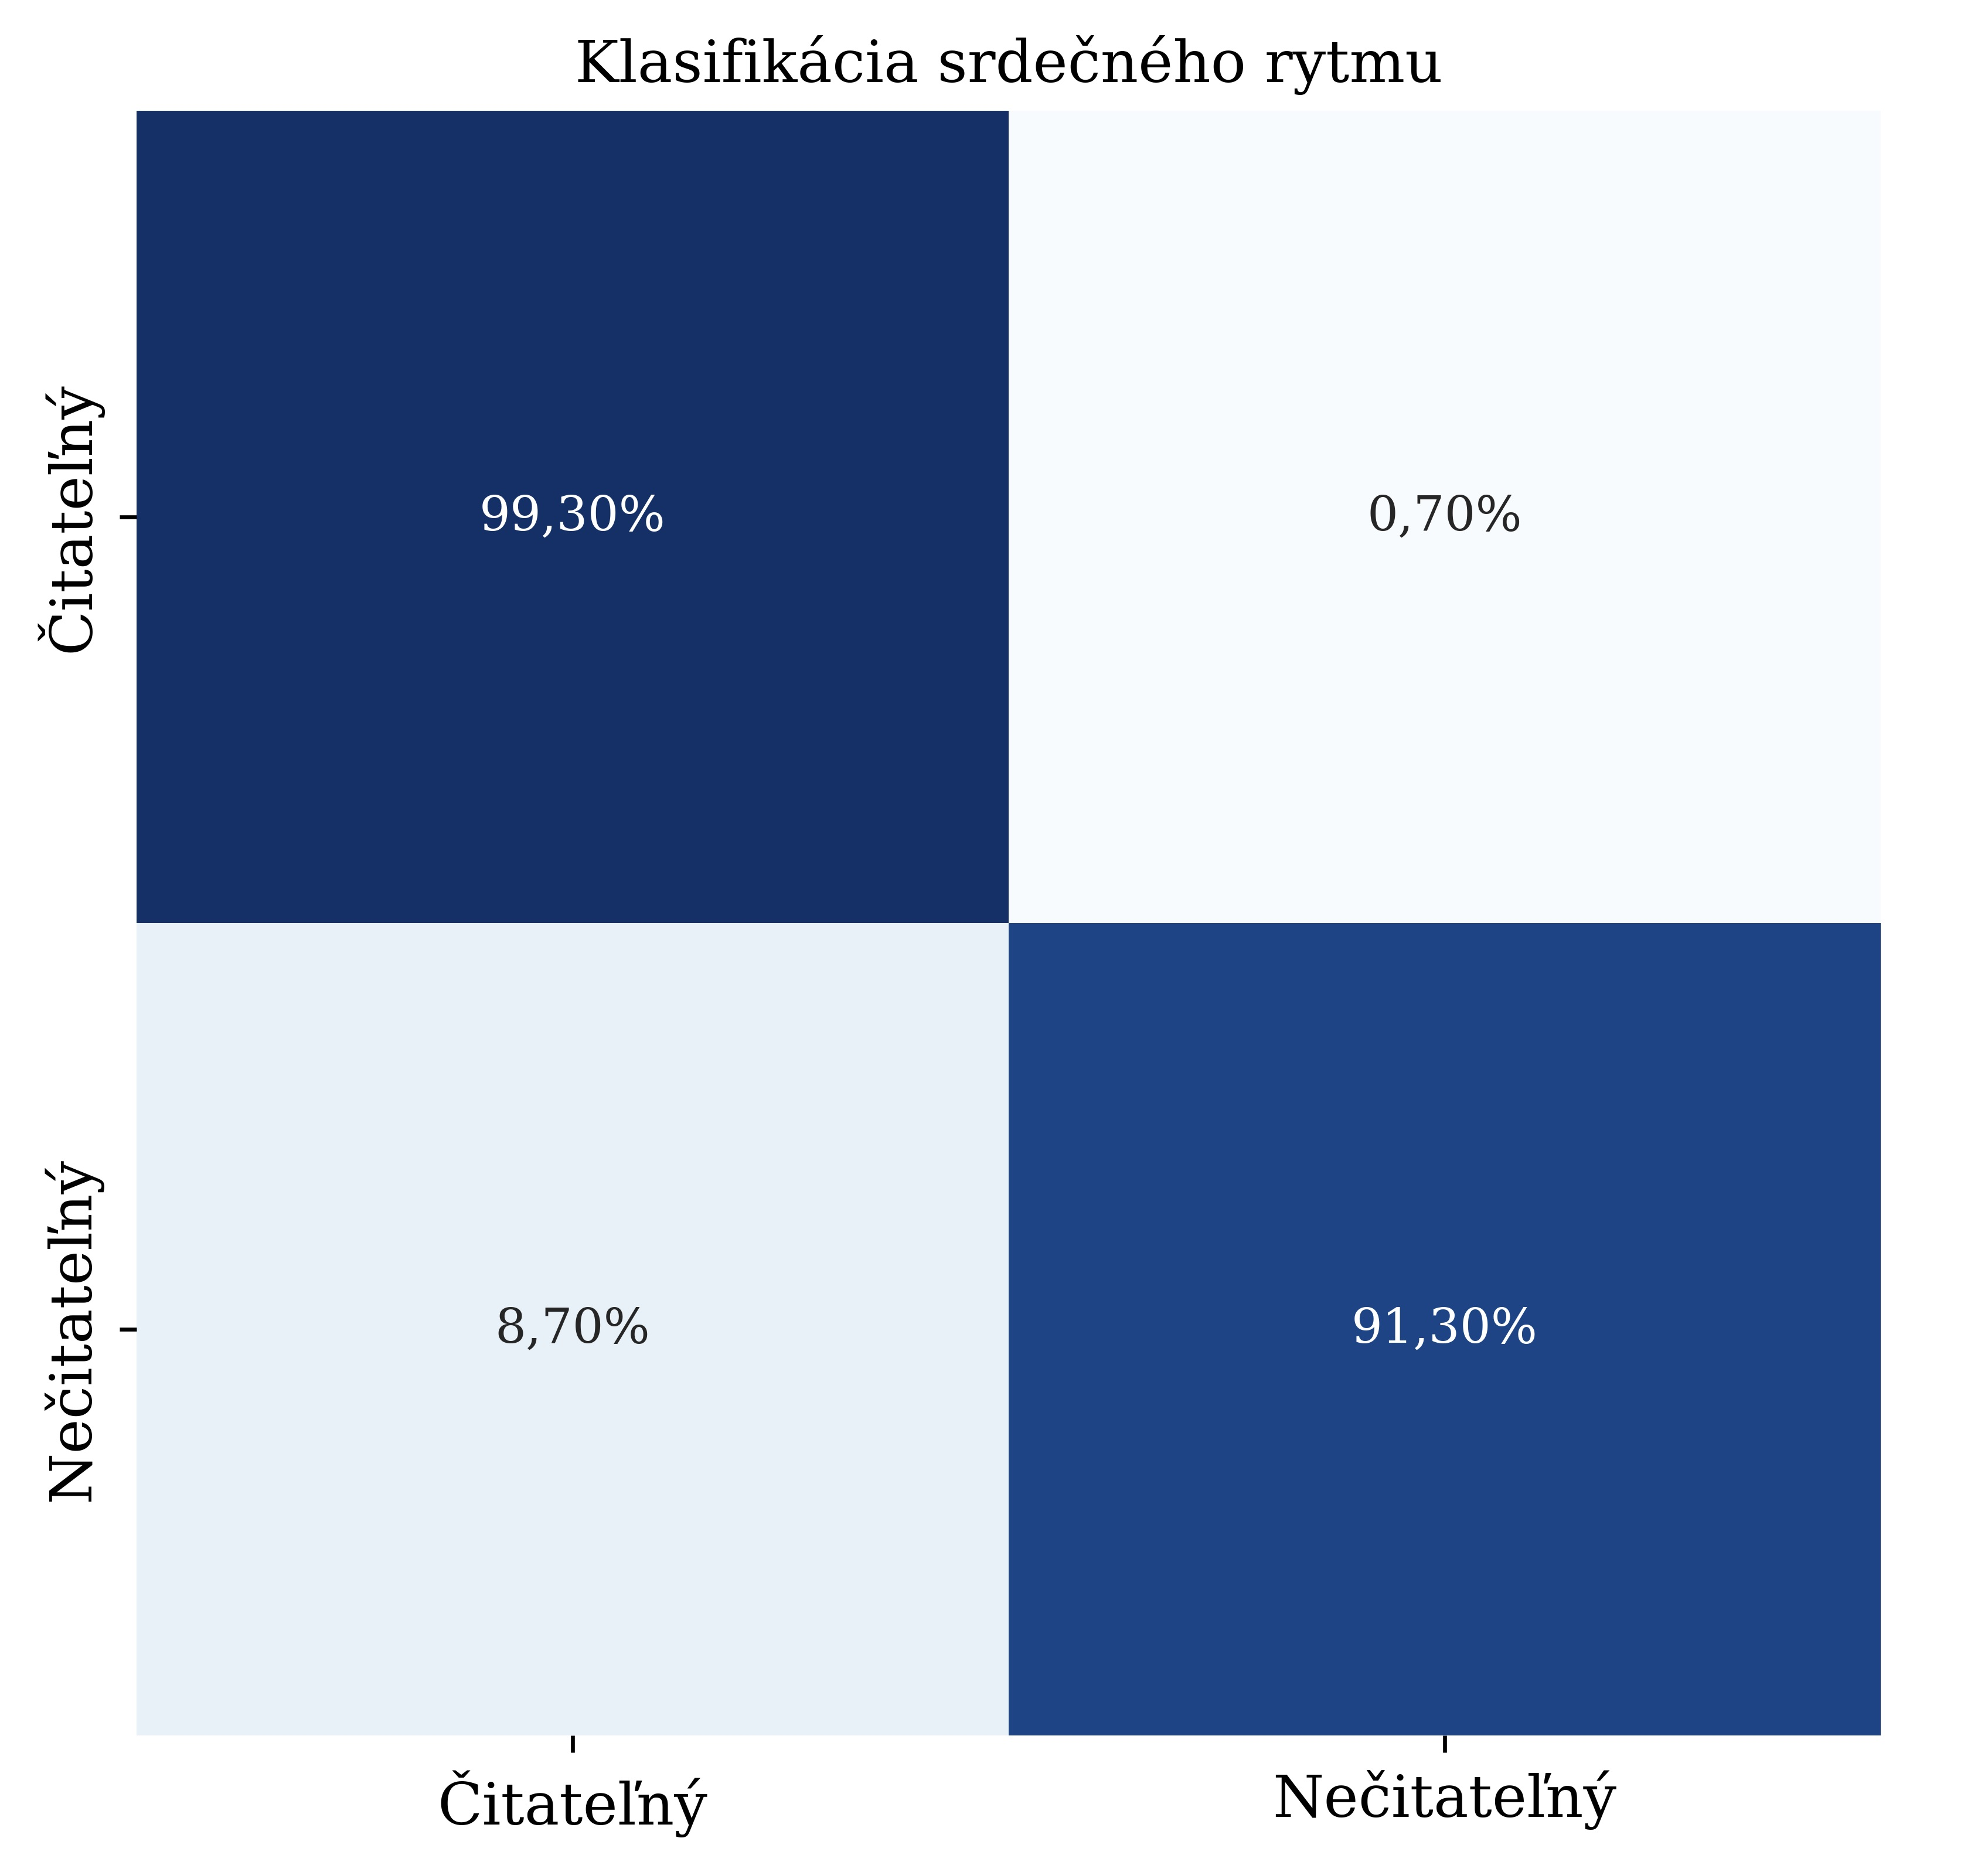
\includegraphics[scale=0.07]{img/confusion_matrix_HR.jpeg}
    \caption{Matica zámen pre klasifikáciu čitateľnosti srdečného rytmu.}
    \label{fig:artefact_classification_HR}
\end{figure}

\begin{table}[H]\centering
\caption[\textit{Precision} a \textit{recall} pre klasifikáciu čitateľnosti srdečného rytmu.]{~\textit{Precision} a \textit{recall} pre klasifikáciu čitateľnosti srdečného rytmu.}\label{tab:artefact_classification_HR}
    \begin{tabular}{l|c|c}
    	\textbf{Srdečný rytmus} & \textit{\textbf{Precision (\%)}} & \textit{\textbf{Recall (\%)}} \tabularnewline \hline 
     	\textbf{Čitateľný}      & 99,30	                      &  99,30                           \tabularnewline \hline
        \textbf{Nečitateľný}	& 91,30	                      &  91,30                          \tabularnewline
    \end{tabular}
\end{table}


Keďže trieda artefaktov je ordinálny príznak, má zmysel pozrieť sa aj na to, o koľko tried sa model pri chybných predikciách mýlil. Pri klasifikácii do štyroch tried sa zo všetkých nesprávnych predikcií model zmýlil o jednu triedu pri \textbf{95,0 \% segmentov} a o dve triedy pri~\textbf{4,4~\% segmentov}. Triedu 1 s triedou 4 zamenil pri predikcii iba v \textbf{0,6 \% segmentov}. Toto opäť značí, že model je schopný naučiť sa charakteristické vlastnosti jednotlivých tried, avšak triedy je potrebné striktnejšie zadefinovať, aby sa minimalizoval počet segmentov na pomedzí dvoch tried.

Kvôli využitiu v reálnom čase je doba, za ktorú dokáže výsledný model predikovať triedu jedného segmentu, dôležitá. Predikciu sme vykonali zvlásť pre každý segment z testovacej množiny dát a výsledné časy spriemerovali. Priemerný čas, ktorý model potrebuje na predikciu jedného segmentu, je \textbf{48 ms}, pričom tento čas je samozrejme závislý na použitom hardware. 


%---------------------------------------------------------------
\chapter{Diskusia}
%---------------------------------------------------------------

Aj keď navrhnutá klasifikácia pohybových artefaktov v rozsahu definovanom zadaním práce funguje, počas návrhu a realizácie riešenia sa nazbieralo veľké množstvo pozorovaní, od ktorých vieme odvodiť možné vylepšenia navrhnutého riešenia. Rozšírenia sa ponúkajú či už v oblasti riadeného experimentu, anotácie dát, alebo skúmania väčšieho množstva architektúr strojového učenia. 

Jedným z rozšírení môže byť využitie dát nameraných v teréne, miesto riadeného experimentu. Takto získané dáta budú bližšie reálnemu využitiu a teda aj výsledný model natrénovaný s~ich pomocou má potenciál zachytiť problém presnejšie. Významným rozdielom oproti riadenému experimentu je napríklad odev, ktorý majú osoby na sebe. Keďže sa predpokladá využitie riešenia pre zložky IZS, najmä hasičov, tieto osoby budú mať na sebe prevažne ťažký odev, v porovnaní s~civilným odevom, aký mali subjekty riadeného experimentu. Ťažký odev v prípade pohybových artefaktov predstavuje ďalší možný zdroj rušenia.

Čo sa týka riadeného experimentu, prirodzeným vylepšením je jeho rozšírenie či~už~z~po-hľadu rozmanitosti pohybových aktivít, alebo množstva dát. Množstvo dát je často rozhodujúce pre kvalitu klasifikácie, čo sme pozorovali aj v tejto práci. Prvé modely sme trénovali priebežne na nameraných dátach, keďže neboli všetky anotované naraz, a presnosť klasifikácie narastala spolu s väčším množstvom dát, rovnako narástla aj keď sme použili validačnú množinu na finálne trénovanie modelu. Väčšie množstvo dát by teda mohlo byť prínosom, pričom okrem zvýšenia počtu subjektov experimentu sa množstvo segmentov dá výrazne zvýšiť aj anotáciou cez kĺzavé okná, čo nás privádza k ďalšej kategórii možných rozšírení navrhnutého riešenia. 

Z hľadiska anotácie dátovej sady sa ponúka niekoľko vylepšení, keďže práve segmenty, ktoré sa nachádzali na pomedzí dvoch tried, sa ukázali ako problematické. Dáta je možné anotovať po kratších oknách, aby sa pravdepodobnosť výskytu viacerých kategórií pohybového artefaktu v jednom segmente znížila. Pri dĺžke kratšej ako 1 sekunda by však už nebolo možné zaručiť, aby každý segment obsahoval jeden celý srdečný cyklus. Lepšou možnosťou môže byť anotácia po jednotlivých srdečných cykloch. Toto riešenie je prácne, lebo vyžaduje robustnú detekciu R-vĺn v zázname a nájdenie riešenia v prípade, že R-vlna nie je z daného úseku rozoznateľná. Kvôli variabilite srdečného cyklu bude navyše potrebné takto získané segmenty prevzorkovať na~jednotnú dĺžku, aby sa dali použiť ako vstupné dáta pre väčšinu modelov umelej inteligencie. Takto zarovnané segmenty môžu byť dobrým základom predikcie v reálnom čase, kedy by sa~miera znečistenia segmentu vyhodnocovala po každom srdečnom cykle. Ďalšou možnosťou je anotácia po úsekoch s variabilnou dĺžkou, kedy by sa dáta anotovali označením časti signálu s vybranou intenzitou rušenia. Takáto anotácia by síce bola najpresnejšia možná, bolo by však treba vyriešiť, ako vhodne vložiť dáta, ktoré nemajú vopred stanovenú dĺžku, na vstup modelu.

Zhodnotenie kvality anotácie je subjektívne a spravidla sa bude líšiť od jednej osoby k~druhej, vyššia miera znalosti interpretácie EKG signálu však môže byť výhodou. Vylepšením z hľadiska správnosti môže teda byť anotácia s asistenciou kardiológa, alebo inej osoby školenej na interpretáciu EKG signálu. Tieto osoby by mali vedieť presnejšie posúdiť, aký veľký vplyv môže mať daná miera znečistenia pohybovým artefaktom na získanie potrebných informácií, či~prípadnú diagnostiku z EKG záznamu.

Okrem vylepšení týkajúcich sa anotácie dátovej sady, priestor na zlepšenie zostáva aj~z~hľadiska optimalizácie počtu tried. Prvé pokusy zahŕňali zlúčenie prostredných dvoch tried do jednej, keďže sa ukázalo, že je medzi nimi veľký prienik. Presnosť predikcií po zlúčení výrazne stúpla, takže ďalšia optimalizácia počtu tried by mohla viesť k presnejším výsledkom. Skúmané počty tried by záviseli od spôsobu anotácie, jednou z možností, ktorá sa ponúka, je rozlíšenie dvoch druhov segmentov aktuálne patriacich do triedy 4 - srdečný rytmus nečitateľný kvôli superponovanému rušeniu, oproti nečitateľnosti kvôli saturácii signálu.

Keďže architektúr strojového učenia je v súčasnosti dostupných mnoho, rozsah tejto práce neumožňoval skúmanie všetkých možností. V tejto práci boli testované rôzne hlboké a~konvolučné architektúry. Priestor zostáva pre zahrnutie LSTM vrstiev \cite{boljanic2022}, ktoré by mohli byť obzvlášť prínosné pre spracovanie časovej zložky vstupných dát, prípadne pre klasifikáciu pomocou SVM modelov \cite{Castao2017}\cite{Kher2015}.



%---------------------------------------------------------------
\chapter{Záver}
%---------------------------------------------------------------


V úvodnej časti práce je spracovaná základná analýza problému, časť o elektrokardiografii pokrý-va rôzne druhy elektród a zvodových systémov, so zameraním na terénnu záťažovú elektrokardiografiu. V krátkosti je opísaná aj genéza signálu a fyziologický priebeh EKG, znalosť ktorého je~potrebná na determinovanie kvality signálu, predstavené sú aj najčastejšie sa vyskytujúce artefakty v EKG signáli a ich pôvod. Práca ďalej obsahuje rešeršnú časť súčasne dostupných riešení automatickej detekcie pohybových artefaktov v oblasti strojového učenia. Popísané sú vybrané postupy v oblasti hlbokých, konvolučných a rekurentných neurónových sietí a klasifikácia pomocou SVM modelov.

Ďalšou časťou práce je návrh riadeného experimentu, ktorý bol realizovaný na desiatich subjektoch. Zaznamenaných bolo päť rôznych pohybových aktivít - kľud, pohyby hornými končatinami, chôdza, beh a drepy. Každá z týchto aktivít bola zaznamenaná troma rôznymi druhmi elektród a to tradičnými Ag/AgCl elektródami, elektródami z chróm-niklovej ocele a~textilnými elektródami. Na zaznamenanie dát bol použitý poskytnutý nositeľný snímač EKG, napojený na 1-zvodový systém. Anotácia dátovej sady bola významnou súčasťou práce, pričom ako výstup vznikol katalóg 4602 anotovaných segmentov o dĺžke 2 sekundy. Nad rámec zadania a~za~účelom zefektívnenia anotácie dát bolo implementované jednoduché grafické rozhranie, ktoré slúži na prehliadanie a anotáciu jednotlivých EKG segmentov. Vzniknutá dátová sada je navyše verejne dostupná pod GNU GPL 3.0 licenciou. 

Prvým výstupom práce je porovnanie vyššie uvedených typov elektród pre účely terén-neho monitorovania. Najodolnejšie voči pohybovým artefaktom vyšli textilné elektródy z vodivej tkaniny upevnené na hrudnom páse. Až 51,9 \% segmentov EKG signálu zaznamenaných pomocou tohto druhu elektród obsahovalo minimálne až žiadne rušenie a iba 3,3 \% segmentov bolo nezlúčiteľných s detekciou srdečného rytmu. 

Ďalším výstupom práce je návrh konvolučnej neurónovej siete, ktorá je schopná klasifikovať jednotlivé pohybové aktivity s presnosťou 85,67 \%. Navrhnutá architektúra bola s menšími úpravami a po vyladení hyperparametrov následne použitá na klasifikáciu pohybových artefaktov. Pri prvotnej definícii obsahujúcej 4 triedy, sme zistili, že prostredné dve majú veľký prienik. Výrazné zlepšenie presnosti sme dosiahli po zlúčení týchto dvoch tried, kedy presnosť klasifikácie na testovacej množine narástla na 87,62 \%. Overili sme aj schopnosť modelu odlíšiť segmenty s~čitateľným a nečitateľným srdečným rytmom, kedy presnosť dosiahla až 98,70 \%.

\newpage

Najväčším problémom sa ukázali byť segmenty, ktoré sa nachádzajú na pomedzí dvoch tried. Toto tvrdenie máme podložené tým, že až v 95 \% nesprávne predikovaných segmentov sa model zmýlil práve o jednu triedu. Pre budúcu optimalizáciu riešenia vidíme niekoľko možných postupov. Jedným by bola precíznejšia anotácia dát, kedy navrhujeme anotáciu po~jednom srdečnom cykle, prípadne anotáciu po úsekoch variabilnej dĺžky. Spolupráca s kardiológom by tiež mohla viesť k presnejšej anotácii. Z hľadiska architektúr hlbokého učenia by mohlo byť prínosné zahrnúť LSTM vrstvy na spracovanie časovej zložky vstupných dát. Čo sa týka implementácie ako relevantnú vidíme možnosť detekcie v reálnom čase, prípadne implementáciu na~vstavaných systémoch s obmedzenými zdrojmi.
 % include `text.tex' from `text/' subdirectory

\appendix\appendixinit % do not remove these two commands

\chapter{Nejaká príloha}


Sem přijde to, co nepatří do hlavní části.
 % include `appendix.tex' from `text/' subdirectory

\backmatter % do not remove this command

\printbibliography % print out the BibLaTeX-generated bibliography list

\chapter{Obsah príloh}
% Concents of the attachment

	\dirtree{%
		.1 readme.txt\DTcomment{stručný popis obsahu média}.
		.1 exe\DTcomment{adresár so spustiteľnou formou implementácie}.
		.1 src.
		.2 impl\DTcomment{zdrojové kódy implementácie}.
		.2 thesis\DTcomment{zdrojová forma práce vo formáte \LaTeX{}}.
		.1 text\DTcomment{text práce}.
		.2 thesis.pdf\DTcomment{text práce vo formáte PDF}.
	}
 % include `medium.tex' from `text/' subdirectory

\end{document}
